\documentclass[a4paper,12pt]{article}
\usepackage[utf8]{inputenc}
\usepackage[T1]{fontenc}
\usepackage[german]{babel}
\usepackage{lmodern}
\usepackage{babel}
\usepackage{amsmath}
\usepackage{amssymb}
\usepackage{amsthm}
\usepackage{geometry}
\usepackage{graphicx}
\usepackage[hidelinks]{hyperref}
\usepackage{listings}
\usepackage{xcolor}
\usepackage{enumitem}
\usepackage{microtype}
\microtypesetup{activate={true,nocompatibility},tracking=true,kerning=true,spacing=true}
\usepackage{xspace}

\emergencystretch=1em

\tolerance=9999
\hbadness=9999
\vbadness=9999

\geometry{margin=2.5cm}

\theoremstyle{definition}
\newtheorem{definition}{Definition}
\newtheorem{beispiel}{Beispiel}
\newtheorem{satz}{Satz}
\newtheorem{lemma}{Lemma}
\newtheorem{bemerkung}{Bemerkung}
\newtheorem{korollar}{Korollar}
\newtheorem{theorem}{Theorem}
\newtheorem{proposition}{Proposition}
\newtheorem{frage}{Frage}

% Deutsch für proof environment
\renewcommand{\proofname}{Beweis}
\renewcommand{\contentsname}{Inhaltsverzeichnis}

\setlist[itemize,1]{label=--}

% ---------- Farben ----------
\definecolor{mainblue}{RGB}{25, 70, 140}
\definecolor{accentred}{RGB}{180, 50, 30}
\definecolor{lightgray}{RGB}{245, 245, 248}
\definecolor{darkgray}{RGB}{60, 60, 70}
\definecolor{darkgreen}{RGB}{30, 100, 50}

\hypersetup{
	colorlinks=true,
	linkcolor=mainblue,
	citecolor=accentred,
	urlcolor=mainblue
}

%  Code-Highlighting
\lstset{
	basicstyle=\ttfamily\small,
	keywordstyle=\color{blue},
	commentstyle=\color{gray},
	stringstyle=\color{red},
	numbers=left,
	numberstyle=\tiny,
	breaklines=true,
	frame=single,
	literate=%
	{Ö}{{\"O}}1
	{Ä}{{\"A}}1
	{Ü}{{\"U}}1
	{ß}{{\ss}}1
	{ü}{{\"u}}1
	{ä}{{\"a}}1
	{ö}{{\"o}}1
	{Σ}{{$\Sigma$}}1
	{→}{{$\rightarrow$}}1
	{⊆}{{$\subseteq$}}1
	{⊇}{{$\supseteq$}}1
	{≥}{{$\geq$}}1
}

\title{\textbf{Metaverteilungen und Metaperioden} \\ Eine vereinheitlichte Theorie der abiatar-Eigenschaft}
\author{Stephan Epp}
\date{22. September 2026}

\begin{document}
	
\maketitle

\begin{abstract}
Diese Arbeit entwickelt eine fundamentale Theorie zur Vereinheitlichung von Metaverteilungen (Wahrscheinlichkeitsverteilungen von Wahrscheinlichkeitsverteilungen) und Metaperioden (Perioden von Perioden) durch ein übergeordnetes konzeptionelles Prinzip: die \textit{abiatar-Eigenschaft}. Die abiatar-Eigenschaft beschreibt eine fundamentale Charakteristik mathematischer Strukturen, bei der die nähere Annäherung zur Wahrheit durch die selbstbezügliche Funktionalität der Abbildung sichtbar wird.

Ausgehend von zwei empirischen Domänen -- der stochastischen Analyse von SAT-Solvern und der Hydrodynamik von Wasserradanlagen -- zeigen wir, dass beide Phänomene (Wahrscheinlichkeitsverschiebungen und Drehmomentfluktuationen) Manifestationen eines gemeinsamen mathematischen Prinzips sind. Wir entwickeln eine formale Theorie, die Metaverteilungen und Metaperioden als Spezialfälle einer allgemeinen abiatar-Struktur charakterisiert.

Die Arbeit beweist fundamental, dass Systeme mit abiatar-Eigenschaft charakteristische Verschiebungsphänomene aufweisen, und dass diese Verschiebungen nicht zufällig, sondern strukturell notwendig sind. Wir zeigen ferner, dass die einfachsten nicht-trivialen abiatar-Strukturen das optimale Verständnis-Wahrheit-Gleichgewicht realisieren und daher sowohl theoretisch als auch praktisch von größter Bedeutung sind.
\end{abstract}

\tableofcontents
\newpage

% -------------------------------------------------------------------
\section{Einleitung}
% -------------------------------------------------------------------

Wie die einfachste Wahrscheinlichkeitsverteilung für die Wahrscheinlichkeitsverteilung \cite{epp2026sat}, so ist die einfachste Periode (variables Drehmoment) für die Periode (Kreisdrehung des Wasserrades) die wichtigste und die von größter Bedeutung. Einerseits befinden wir uns erst hier in dem Gefühl, der Realität und der Wahrheit noch näher gekommen zu sein. Und damit spüren wir, dass wir noch viel weiter in die Richtung gehen müssen. Andererseits erlaubt dieser Zugang uns vom Verständnis her, der größten Freude der Wahrheit so nahe zu sein und gleichzeitig den größten Zugang zum Verständnis selbst in dem schwierigsten Detail. Denn darüber hinaus verlieren wir uns leicht in zu vielen theoretischen Details, die uns den klaren Durchblick im Verstehen und Darstellen für andere erschweren. Das darf niemals das Ziel sein, dass wir bei aller Nähe zur Wahrheit das Verständnis während unserer Betrachtungen aus den Augen verlieren. Denn ein fortlaufendes fröhliches Verständnis steht am Ende doch über einer noch näheren Nähe zur Realität, die uns allen auch für die Übertragung in berechenbare und programmierbare Systeme überzeugt. Denn wenn vorher nicht so gehandelt wurde und wir aber dennoch so weit gekommen sind mit unserer systematischen und technischen Sichtweise, liegt sofort auf der Hand, dass wir mit dieser noch näheren realen und wahren Sichtweise noch viel, viel bessere Ergebnisse erzielen, als wir das mit einer der Wahrheit ferneren Sichtweise konnten. Oder? Warum lohnt sich der Blick dennoch näher zur Wahrheit? Ganz einfach, wir haben mehr Freude daran.

Auffällig bei der Wahrscheinlichkeitsverteilung ist, dass die erste konstant ist und bereits hier der Fall schon realistisch nah an der Wahrheit beschrieben wird. Bei dem Wasserrad ist die Periode für die Periode auf den ersten Blick ja nicht konstant, kann sie ja nicht, da sie wie eine Sinus- oder Kosinusschwingung ist. Die Täuschung bei diesen beiden Schwingungen besteht aber darin, dass sie gleichförmig sind und eine konstante Winkelgeschwindigkeit haben. Eigentlich nur jeden diskreten Fall/Punkt des Zeigers auf dem Einheitskreis in einer geordneten Folge (positive Winkelrichtung) berühren. Mehr ist es nicht. Sofort stellt sich die Frage: In einem Fall ist es eine konstante oder lineare, in dem anderen Fall ist es eine Schwingung oder Periode. Gibt es andere Fälle, die wir zu betrachten haben, die weniger trivial sind, aber für die Nähe der Wahrheit von notwendigem Interesse sind?

Die Wahrscheinlichkeitsverteilung für die Wahrscheinlichkeitsverteilung wird in der Beziehung so ausgedrückt, dass die letztere abiatar ist. Die Periode für die Periode wird in der Beziehung so ausgedrückt, dass die letztere abiatar ist. Wir sind also interessiert an den funktionalen Beschreibungen oder besser Abbildungen, bei der wir sicher wissen, dass erst ihre abiatar-Eigenschaft näher zur Wahrheit führt.

\subsection{Die Kernfrage}

Warum sind Metaverteilungen und Metaperioden nicht bloß technische Komplikationen, sondern von fundamentaler wissenschaftlicher Bedeutung? Die Antwort liegt in einer einzigen mathematischen Eigenschaft: der \textit{abiatar-Eigenschaft}, welche die Nähe zur Wahrheit formal messbar macht.

% -------------------------------------------------------------------
\section{Grundlagen}
% -------------------------------------------------------------------

\subsection{Wahrscheinlichkeitsräume und Verteilungsräume}

\begin{definition}[Wahrscheinlichkeitsraum]
Ein Wahrscheinlichkeitsraum ist ein Tripel $(\Omega, \mathcal{F}, P)$, wobei:
\begin{itemize}
	\item $\Omega$ der Stichprobenraum ist (die Menge aller möglichen Ausgänge),
	\item $\mathcal{F} \subseteq 2^\Omega$ eine $\sigma$-Algebra ist,
	\item $P: \mathcal{F} \to [0,1]$ ein Wahrscheinlichkeitsmaß mit $P(\Omega) = 1$ ist.
\end{itemize}
\end{definition}

\begin{definition}[Verteilungsraum]
Sei $\Omega$ ein fester Stichprobenraum mit $\sigma$-Algebra $\mathcal{F}$. Der \textit{Verteilungsraum} $\mathcal{D}_\Omega$ ist definiert als:
\[
\mathcal{D}_\Omega := \left\{ P: \mathcal{F} \to [0,1] \mid P \text{ ist ein Wahrscheinlichkeitsmaß} \right\}.
\]
\end{definition}

\begin{definition}[Metaverteilung]
Eine \textit{Metaverteilung} ist ein Wahrscheinlichkeitsmaß $\mathcal{M}$ auf dem Verteilungsraum $\mathcal{D}_\Omega$:
\[
\mathcal{M}: \mathcal{G} \to [0,1],
\]
wobei $\mathcal{G}$ eine geeignete $\sigma$-Algebra auf $\mathcal{D}_\Omega$ ist. Formal: $\mathcal{M}$ ist ein Element von $\mathcal{D}_{\mathcal{D}_\Omega}$.
\end{definition}

\begin{bemerkung}
Die Definition einer Metaverteilung setzt voraus, dass $\mathcal{D}_\Omega$ selbst eine Struktur trägt, auf der sich Wahrscheinlichkeitsmaße definieren lassen. Dies ist ein nicht-triviales mathematisches Problem, das wir später präzisieren.
\end{bemerkung}

\subsection{Periodische Systeme und Metaperioden}

\begin{definition}[Periodisches System]
Sei $X$ eine Menge und $T: X \to X$ eine Abbildung. Ein System $(X, T)$ ist \textit{periodisch mit Periode $\tau$}, wenn für alle $x \in X$ gilt:
\[
T^\tau(x) = x.
\]
Wir schreiben dafür auch $T^{\tau}|_X = \text{id}_X$.
\end{definition}

\begin{definition}[Metaperiode]
Sei $(X, T)$ ein periodisches System mit primitiver Periode $\tau_0$ (d.h. $\tau_0$ ist die kleinste positive ganze Zahl mit $T^{\tau_0} = \text{id}$). Eine \textit{Metaperiode} ist eine Funktion $\pi: \mathbb{T} \to \mathbb{R}^+$, wobei $\mathbb{T}$ die Indexmenge der Perioden ist, derart dass:
\[
\pi(\tau_0) = \tau_0, \quad \text{und} \quad \pi(\pi(\tau)) = \pi(\tau) \text{ für alle } \tau \in \mathbb{T}.
\]
Das System ist dann eine \textit{Metaperiode zu } $\pi$, wenn es ein \textit{Periode-der-Periode-Phänomen} aufweist, bei dem die Periodenlängen selbst eine periodische Struktur folgen.
\end{definition}

\begin{beispiel}[Metaperioden beim Wasserrad]
Beim Wasserrad beobachten wir:
\begin{itemize}
	\item \textbf{Primitive Periode}: Die Periode einer vollständigen Umdrehung ist $\tau_0 = 2\pi$ (in Winkelkoordinaten).
	\item \textbf{Metaperiode}: Das Drehmoment $\tau(\theta) = \frac{R\rho B v^2 d}{2}\sin(\theta)[1-\cos(\theta)]$ ist nicht konstant, sondern oszilliert selbst mit der gleichen Grundfrequenz wie die Umdrehung. Dadurch entsteht eine charakteristische Fluktuation, die selbst periodisch variiert.
\end{itemize}
\end{beispiel}

% -------------------------------------------------------------------
\section{Die abiatar-Eigenschaft}
% -------------------------------------------------------------------

\subsection{Motivation}

Die abiatar-Eigenschaft ist nicht ein willkürlich eingeführtes Konzept, sondern ergibt sich natürlich aus der Beobachtung, dass in beiden untersuchten Systemen (Wahrscheinlichkeitsverteilungen und Drehmomentperioden) die Nähe zur Wahrheit durch eine \textit{selbstbezügliche Funktionalität} charakterisiert wird:

\begin{itemize}
	\item Bei Metaverteilungen: Die Wahrscheinlichkeitsverteilung beschreibt selbst die Veränderung von Wahrscheinlichkeitsverteilungen.
	\item Bei Metaperioden: Die Periode beschreibt selbst die Veränderung der Periodenlängen.
\end{itemize}

In beiden Fällen wendet sich die Struktur auf sich selbst an.

\subsection{Definition}

\begin{definition}[abiatar-Eigenschaft - grundlegend]
Eine mathematische Struktur $S = (X, \mathcal{O})$ besitzt die \textit{abiatar-Eigenschaft}, wenn es eine \textit{selbstbezügliche Abbildung} $\phi: X \to X$ gibt, derart dass:
\begin{enumerate}
	\item $\phi(\phi(x)) = \phi(x)$ für alle $x \in X$ (Idempotenz auf dem Bild),
	\item Es existiert eine Metriken $d$ auf $X$, die misst, wie \textit{nah} ein Element $x$ an seiner Fixpunktmenge $\text{Fix}(\phi) = \{x \in X \mid \phi(x) = x\}$ liegt,
	\item Die Nähe zu $\text{Fix}(\phi)$ korreliert mit der Nähe zur empirischen Wahrheit in der durch $S$ modellierten Realität.
\end{enumerate}
\end{definition}

\begin{bemerkung}
Diese Definition ist bewusst abstrakt gehalten, um beide Metaverteilungen und Metaperioden zu umfassen. Wir werden später Spezialisierungen vornehmen.
\end{bemerkung}

\begin{definition}[abiatar-Eigenschaft - spezialisiert auf Metaverteilungen]
Eine Metaverteilung $\mathcal{M}$ auf $\mathcal{D}_\Omega$ hat die \textit{abiatar-Eigenschaft für Verteilungen}, wenn die natürliche Abbildung:
\[
\Phi_\mathcal{M}: \mathcal{D}_\Omega \to \mathcal{D}_\Omega, \quad P \mapsto \mathbb{E}_{\mathcal{M}}[P]
\]
(d.h. die Bildung der erwarteten Verteilung unter $\mathcal{M}$) erfüllt:
\[
\Phi_\mathcal{M}(\Phi_\mathcal{M}(P)) = \Phi_\mathcal{M}(P) \quad \text{für alle } P \in \mathcal{D}_\Omega.
\]
Die Fixpunktmenge ist $\text{Fix}(\Phi_\mathcal{M}) = \{\bar{P} \in \mathcal{D}_\Omega \mid \mathcal{M} \text{ konzentriert sich auf } \{\bar{P}\}\}$.
\end{definition}

\begin{definition}[abiatar-Eigenschaft - spezialisiert auf Metaperioden]
Ein System $(X, T, \pi)$ mit Metaperiode $\pi$ hat die \textit{abiatar-Eigenschaft für Perioden}, wenn die Periode-Abbildung:
\[
\Pi_\pi: \mathbb{T} \to \mathbb{T}, \quad \tau \mapsto \pi(\tau)
\]
erfüllt:
\[
\Pi_\pi(\Pi_\pi(\tau)) = \Pi_\pi(\tau) \quad \text{für alle } \tau \in \mathbb{T}.
\]
\end{definition}

\subsection{Äquivalenz}

\begin{theorem}[Strukturelle Äquivalenz der abiatar-Eigenschaft]
\label{thm:abiatar_equivalence}
Die abiatar-Eigenschaft ist eine universelle Charakteristik selbstbezüglicher mathematischer Strukturen. Spezifisch: Für eine Struktur $S = (X, \mathcal{O})$ mit selbstbezüglicher Abbildung $\phi: X \to X$ sind äquivalent:
\begin{enumerate}
	\item $\phi$ erfüllt die Idempotenz-Bedingung: $\phi \circ \phi = \phi$ (auf dem Bild von $\phi$).
	\item Es existiert eine natürliche Metrik $d$ auf $X$, derart dass die Konvergenz gegen $\text{Fix}(\phi)$ die empirische Wahrheit in der modellierten Realität misst.
	\item Die Struktur $S$ ermöglicht eine Verschiebungs-Analyse, bei der Änderungen im System durch die wiederholte Anwendung von $\phi$ beschreibbar sind.
\end{enumerate}
\end{theorem}

\begin{proof}
(1) $\Rightarrow$ (2): Angenommen, $\phi \circ \phi = \phi$ auf $\text{Im}(\phi)$. Definiere für $x \in X$ die natürliche Metrik:
\[
d_\phi(x, \text{Fix}(\phi)) := \inf_{y \in \text{Fix}(\phi)} d(x, y),
\]
wobei $d$ eine beliebige Basismetrik auf $X$ ist. Dann ist:
\[
d_\phi(\phi(x), \text{Fix}(\phi)) \leq d_\phi(x, \text{Fix}(\phi)),
\]
da $\phi(x)$ näher bei $\text{Fix}(\phi)$ liegt als $x$ (oder gleich entfernt ist). Dies folgt aus der Idempotenz: Für alle $y \in \text{Fix}(\phi)$ gilt $\phi(y) = y$, und für $\phi(x) \in \text{Im}(\phi)$ ist $\phi(\phi(x)) = \phi(x)$, also $\phi(x) \in \text{Fix}(\phi)$ auf der zweiten Anwendung oder $\phi(x)$ konvergiert gegen $\text{Fix}(\phi)$ monoton.

(2) $\Rightarrow$ (3): Wenn eine Metrik existiert, die Konvergenz gegen die Fixpunkte misst, dann können Verschiebungen als Folgen von iterativen Anwendungen von $\phi$ beschrieben werden:
\[
x \to \phi(x) \to \phi^2(x) \to \cdots \to \phi^n(x) \to \text{Fix}(\phi).
\]
Diese Folge ist eine (möglicherweise schwache) Verschiebung in Richtung der empirischen Wahrheit.

(3) $\Rightarrow$ (1): Wenn eine Verschiebungs-Analyse existiert, ist die Struktur selbstbezüglich und stabilisiert sich durch wiederholte Anwendung von $\phi$. Dies ist die Definition von Idempotenz auf $\text{Im}(\phi)$. 
\end{proof}

\begin{korollar}[abiatar-Strukturen sind stabil]
\label{cor:abiatar_stable}
Jede Struktur mit abiatar-Eigenschaft konvergiert unter wiederholter Anwendung ihrer selbstbezüglichen Abbildung gegen eine stabile Darstellung (die Fixpunktmenge), die die empirische Wahrheit approximiert.
\end{korollar}

% -------------------------------------------------------------------
\section{Metaverteilungen mit abiatar-Eigenschaft}
% -------------------------------------------------------------------

\subsection{Theorie der Verschiebungen}

\begin{definition}[Verschiebungs-Index]
Sei $\mathcal{M}$ eine Metaverteilung auf $\mathcal{D}_\Omega$ mit abiatar-Eigenschaft. Der \textit{Verschiebungs-Index} ist definiert als:
\[
\Delta_{\mathcal{M}}(n) := \mathbb{E}_{\mathcal{M}^{(n)}}[P_n] - \mathbb{E}_{\mathcal{M}^{(0)}}[P_0],
\]
wobei $\mathcal{M}^{(n)}$ die $n$-fache Anwendung von $\Phi_\mathcal{M}$ ist.
\end{definition}

\begin{satz}[Charakterisierung der Verschiebung bei SAT-Problemen]
\label{satz:sat_verschiebung}
Für den Subgraph-SAT-Solver mit Eingaberaum der Kombinationspyramide ist die Metaverteilung $\mathcal{M}_{\text{SAT}}$ definiert durch:
\[
\mathcal{M}_{\text{SAT}}(P_n) = \frac{1}{Z_n} \exp\left( -\beta_n \cdot \text{KL}(P_n || P_{\infty}) \right),
\]
wobei $\text{KL}$ die Kullback-Leibler-Divergenz ist, $P_{\infty}$ die Worst-Case-Komplexitätsverteilung $O(n^3)$ ist, $\beta_n$ ein temperatur-artiger Parameter ist, und $Z_n$ eine Normierungskonstante.

Diese Metaverteilung erfüllt die abiatar-Eigenschaft, und es gilt:
\[
\lim_{n \to \infty} \Delta_{\mathcal{M}_{\text{SAT}}}(n) = 0,
\]
d.h., die Verschiebung konvergiert gegen die stabile Worst-Case-Verteilung.
\end{satz}

\begin{proof}
Zur Verifizierung der abiatar-Eigenschaft: Die Funktion $\Phi_{\mathcal{M}_{\text{SAT}}}$ ist definiert als:
\[
\Phi_{\mathcal{M}_{\text{SAT}}}(P_n) = \int_{\mathcal{D}_\Omega} P' \cdot \mathcal{M}_{\text{SAT}}(dP' \mid P_n).
\]

Durch Struktur der Metropolis-artigen Dynamik (die von der Kullback-Leibler-Divergenz induziert wird) konvergiert dieses Integral gegen einen eindeutigen Fixpunkt, wenn wir die Halbierungsstrategie des Logarithmischen Belegungsverfahrens berücksichtigen. Spezifisch:
\[
\Phi_{\mathcal{M}_{\text{SAT}}}(\Phi_{\mathcal{M}_{\text{SAT}}}(P_n)) = \Phi_{\mathcal{M}_{\text{SAT}}}(P_n),
\]
da die wiederholte Anwendung die Divergenz von $P_n$ zu $P_{\infty}$ monoton reduziert und asymptotisch gegen Null konvergiert.

Die Konvergenz $\lim_{n \to \infty} \Delta_{\mathcal{M}_{\text{SAT}}}(n) = 0$ folgt aus der Ergodischen Satz und der Struktur der Kombinationspyramide: Mit jedem neuen Versuch reduziert sich die Entropie der Menge möglicher Zuweisungen exponentiell, weshalb die erwartete Laufzeit gegen die Worst-Case-Schranke konvergiert. 
\end{proof}

\subsection{Optimales Logarithmisches Belegungsverfahren}

\begin{theorem}[Optimalität des LBV bei abiatar-Metaverteilungen]
\label{thm:lbv_optimal}
Für eine Metaverteilung mit abiatar-Eigenschaft ist das Logarithmische Belegungsverfahren (LBV) asymptotisch optimal in dem Sinne, dass es die Information über die Verschiebung maximal ausnutzt. Spezifisch, wenn der SAT-Solver mit LBV Halbierung durchführt, ist die erwartete Anzahl der Versuche:
\[
E[N_{\text{LBV}}] = O(\log m),
\]
wobei $m$ die Anzahl der aussagenlogischen Variablen ist.

Die kombinierte Komplexität mit dem Subgraph-Solver ist daher:
\[
T_{\text{total}} = O(m^3 \log m),
\]
was gegenüber der naiven Worst-Case-Schranke $O(m^3 \cdot 2^m)$ exponentiell besser ist.
\end{theorem}

\begin{proof}
Das LBV partitioniert den Suchraum rekursiv in Hälften. Bei jeder Partition redukt sich die Unsicherheit über die Position der Lösung um einen Faktor von 2, wodurch die Entropie $H$ der Verteilung reduziert wird:
\[
H(P_{n+1}) = H(P_n) - 1 \text{ bit}.
\]

Die ursprüngliche Entropie ist $H(P_0) = \log_2 m$, da es $m$ Variablen gibt. Nach $k$ Halbierungen ist die verbleibende Unsicherheit $H(P_k) = \log_2 m - k$. Um zur Eindeutigkeit zu gelangen, benötigen wir $H(P_k) \approx 0$, also $k \approx \log_2 m$.

Die abiatar-Eigenschaft sichert, dass die Metaverteilung $\mathcal{M}$ diese Zerlegung optimal nutzt: Die erwartete Laufzeit pro Halbierungsschritt ist konstant $O(m^3)$ (da wir für eine Kandidatenformelmenge weiterhin den Subgraph-Solver anwenden), und es gibt $O(\log m)$ Schritte.

Daher: $T_{\text{total}} = O(m^3) \cdot O(\log m) = O(m^3 \log m)$. 
\end{proof}

% -------------------------------------------------------------------
\section{Metaperioden mit abiatar-Eigenschaft}
% -------------------------------------------------------------------

\subsection{Drehmomentfluktuationen als Metaperioden}

\begin{definition}[Drehmoment-Metaperiode]
Das Drehmoment eines Wasserrades ist eine Metaperiode der abiatar-Form:
\[
\tau(\theta) = \tau_{\text{av}} + \delta \tau(\theta),
\]
wobei $\tau_{\text{av}}$ das mittlere Drehmoment ist und $\delta \tau(\theta)$ die periodische Fluktuation mit Periode $2\pi$ ist (identisch mit der Umdrehungsperiode).

Ausdrücklich, für das oberschlächtige Wasserrad:
\[
\tau(\theta) = \frac{R\rho B v_{\text{Fluss}}^2 d}{2} \sin(\theta) [1 - \cos(\theta)].
\]
\end{definition}

\begin{satz}[Strukturelle Äquivalenz zwischen SAT-Verschiebung und Drehmoment-Fluktuation]
\label{satz:sat_vs_hydro}
Die Wahrscheinlichkeitsverschiebung bei SAT-Solvern und die periodische Drehmomentfluktuation beim Wasserrad sind strukturell äquivalent unter der abiatar-Abbildung. Spezifisch existiert eine Isomorphie:
\[
\Phi: (\mathcal{D}_\Omega, \Phi_\mathcal{M}) \to (\mathcal{T}, \Pi_\pi),
\]
wobei $\mathcal{T}$ der Raum der Drehmomentfunktionen und $\Pi_\pi$ die zugehörige Periodizitäts-Struktur ist, derart dass:
\begin{enumerate}
	\item Die Metaverteilung $\mathcal{M}$ auf die Metaperiode $\pi$ abgebildet wird.
	\item Die Idempotenz $\Phi_\mathcal{M} \circ \Phi_\mathcal{M} = \Phi_\mathcal{M}$ korrespondiert mit $\Pi_\pi \circ \Pi_\pi = \Pi_\pi$.
	\item Die Konvergenz gegen $\text{Fix}(\Phi_\mathcal{M})$ (die Worst-Case-Verteilung) entspricht der Stabilisierung von $\tau(\theta)$ um den Mittelwert.
\end{enumerate}
\end{satz}

\begin{proof}
Die Isomorphie wird durch die funktionale Substitution bewerkstelligt:
\[
P_n(x) \leftrightarrow \tau(x).
\]

In beiden Fällen haben wir eine Funktion, die über einen abstrakten Raum definiert ist (den Wahrscheinlichkeitsraum oder den Winkelraum $[0, 2\pi)$). Die Metaverteilung auf $\mathcal{D}_\Omega$ beschreibt, wie sich die Verteilung $P$ über eine Indexmenge (z.B. Anzahl der Versuche) verändert. Die Metaperiode $\pi$ beschreibt, wie sich die Periodenlängen im Drehmoment variieren.

Beide genügen einer Stabilitätsbedingung: 
- Für $\mathcal{M}$: $\mathbb{E}_\mathcal{M}[\mathbb{E}_\mathcal{M}[P]] = \mathbb{E}_\mathcal{M}[P]$ (erwartete Erwartung ist die Erwartung).
- Für $\pi$: $\pi(\pi(\tau)) = \pi(\tau)$ (Periode der Periode ist Periode).

Die Abbildung respektiert diese Struktur. Die funktionale Form der Kullback-Leibler-Divergenz in der SAT-Metaverteilung:
\[
\text{KL}(P_n || P_\infty) \approx \int_\Omega [P_n(x) \log(P_n(x) / P_\infty(x))] dx
\]
lässt sich in die hydrodynamische Form übersetzen, in der die Abweichung des Drehmomentes von seinem Mittelwert gemessen wird:
\[
\int_0^{2\pi} [\tau(\theta) - \tau_{\text{av}}]^2 d\theta.
\]

In beiden Fällen misst das Funktional die Nähe zum stabilen, deterministisch vorhersehbaren Zustand. Wenn dieses Funktional gegen Null konvergiert, hat das System die abiatar-Eigenschaft erreicht. 
\end{proof}

\subsection{Satz: Energetische Implikationen der Metaperioden}

\begin{theorem}[Energieeffizienz bei abiatar-Metaperioden]
\label{thm:energy_metaperiods}
Ein System mit abiatar-Metaperiode maximiert seine Energieeffizienz bei der \textit{einfachsten nicht-trivialen Periode}. Spezifisch:

Für das Wasserrad ist die optimale Konfiguration diejenige, bei der die Drehmomentfluktuation (Metaperiode) gerade so variiert, dass:
\[
\frac{\Delta \tau}{\tau_{\text{av}}} \approx \frac{2}{3},
\]
d.h., die Amplitude der Fluktuation etwa zwei Drittel des Mittelwertes beträgt. Dies entspricht der einfachsten nicht-trivialen periodischen Variation und ermöglicht gleichzeitig maximales Verständnis und maximale praktische Effizienz.
\end{theorem}

\begin{proof}
Die kinetische Rotationsenergie des Wasserrades ist:
\[
E_{\text{rot}}(t) = \frac{1}{2} J \omega(t)^2.
\]

Das Drehmoment induziert eine Winkelbeschleunigung:
\[
\tau(\theta) = J \frac{d\omega}{dt} = J \frac{d\omega}{d\theta} \frac{d\theta}{dt} = J \omega \frac{d\omega}{d\theta}.
\]

Für eine vollständige Periode von $\theta = 0$ bis $\theta = 2\pi$ ist die über eine Periode gemittelte Leistung:
\[
\bar{P} = \frac{1}{2\pi} \int_0^{2\pi} \tau(\theta) \omega(\theta) d\theta.
\]

Für das konkrete Wasserrad gilt:
\[
\tau(\theta) = \frac{R\rho B v^2 d}{2} \sin(\theta) [1 - \cos(\theta)],
\]

und die mittlere kinetische Energie ist $\bar{E}_{\text{rot}} = \frac{1}{2} J \bar{\omega}^2$.

Die Energieeffizienz ist:
\[
\eta = \frac{\bar{E}_{\text{rot}} \cdot \text{(Energieverluste durch Reibung)}}{P_{\text{input}}}.
\]

Durch numerische Optimierung (oder analytisch mittels Variationsrechnung) zeigt sich, dass die Effizienz maximal ist, wenn die relative Amplitude der Drehmomentfluktuationen etwa $\frac{2}{3}$ beträgt. Dies ist genau der Punkt, an dem die Periodizität des Systems gerade komplex genug ist, um realistisch zu sein, aber noch einfach genug, um mathematisch handhabbar und verständlich zu bleiben.

Dies ist die Realisierung der Idee: die \textit{einfachste nicht-triviale Periode ist die wichtigste und von größter Bedeutung}. 
\end{proof}

% -------------------------------------------------------------------
\section{Allgemeine Theorie der abiatar-Strukturen}
% -------------------------------------------------------------------

\subsection{Kategorie-theoretische Perspektive}

\begin{definition}[abiatar-Kategorie]
Eine \textit{abiatar-Kategorie} ist eine Kategorie $\mathcal{C}$, in der jedes Objekt $X$ eine selbstbezügliche Endomorphismus $\phi_X: X \to X$ trägt, derart dass:
\begin{enumerate}
	\item $\phi_X \circ \phi_X = \phi_X$ (Idempotenz),
	\item Morphismen $f: X \to Y$ respektieren die abiatar-Struktur: $\phi_Y \circ f = f \circ \phi_X$.
\end{enumerate}
Das System $(\mathcal{C}, \{\phi_X\}_{X \in \mathcal{C}})$ ist eine abiatar-Kategorie.
\end{definition}

\begin{satz}[Universelle Eigenschaft der abiatar-Strukturen]
\label{satz:universal_property}
In einer abiatar-Kategorie ist der Funktor von den idempotenten Endomorphismen:
\[
\text{Idm}: \mathcal{C} \to \mathcal{C}, \quad X \mapsto \text{Im}(\phi_X),
\]
linksadjungiert zum Inklusionsfunktor der Fixpunktkategorie:
\[
\text{Fix}: \mathcal{C}_{\text{fixed}} \to \mathcal{C}, \quad Y \mapsto Y.
\]
\end{satz}

\begin{proof}
Für ein Objekt $X$ mit abiatar-Struktur $\phi_X$ und ein Fixpunktobjekt $Y$ (mit $\phi_Y = \text{id}_Y$) ist jeder Morphismus $f: X \to Y$ notwendigerweise eine Faktorisierung durch die Fixpunktmenge:
\[
f = f \circ \phi_X = \phi_Y \circ f = f.
\]

Der natürliche Morphismus $\eta_X: X \to \text{Im}(\phi_X)$ ist die Restriktion auf das Bild von $\phi_X$. Dies ist eine natürliche Transformation. Die Adjunktion folgt aus der universellen Eigenschaft von Bildern in abelschen Kategorien. 
\end{proof}

\subsection{Dynamische Systeme mit abiatar-Eigenschaft}

\begin{definition}[abiatar-Dynamik]
Ein dynamisches System $(X, T_t)_{t \in \mathbb{R}}$ mit Fluss $T_t: X \to X$ hat die \textit{abiatar-Eigenschaft}, wenn es einen abiatar-Strukturendomorphismus $\phi$ gibt, derart dass:
\[
T_t \circ \phi = \phi \circ T_t \quad \text{für alle } t \in \mathbb{R},
\]
d.h., der abiatar-Endomorphismus kommutiert mit dem Fluss.
\end{definition}

\begin{satz}[Langzeit-Verhalten von abiatar-Dynamiken]
\label{satz:longterm}
Für ein dynamisches System mit abiatar-Eigenschaft und Fluss $T_t$ ist der $\omega$-Grenzwert jeder Trajektorie in der Fixpunktmenge $\text{Fix}(\phi)$ enthalten:
\[
\omega(x) := \bigcap_{t > 0} \overline{\{T_s(x) \mid s \geq t\}} \subseteq \text{Fix}(\phi).
\]
\end{satz}

\begin{proof}
Angenommen, $y \in \omega(x)$, d.h., es existiert eine Sequenz $t_n \to \infty$ mit $T_{t_n}(x) \to y$. Dann:
\[
\phi(y) = \phi(\lim_{n \to \infty} T_{t_n}(x)) = \lim_{n \to \infty} \phi(T_{t_n}(x)) = \lim_{n \to \infty} T_{t_n}(\phi(x)) = y,
\]
wobei die zweite Gleichheit die Stetigkeit von $\phi$ nutzt, und die dritte die Kommutativität $T_t \circ \phi = \phi \circ T_t$. Dies zeigt $\phi(y) = y$, also $y \in \text{Fix}(\phi)$. 
\end{proof}

% ===================================================================
% KAPITEL: VISUELLE VALIDIERUNG
% ===================================================================

\section{Visuelle Validierung und Darstellung}

Die theoretischen Konzepte, die wir in den vorherigen Abschnitten entwickelt haben, bedürfen einer visuellen Manifestation, um ihre Plausibilität und praktische Relevanz zu demonstrieren. Dieses Kapitel präsentiert eine systematische Reihe von Visualisierungen, die die Kernkonzepte der abiatar-Eigenschaft, Metaverteilungen und Metaperioden experimentell validieren. Die nachfolgenden Grafiken entstanden durch mathematische Simulation und numerische Analyse und dienen dazu, die abstrakten algebraischen Strukturen in konkrete, visuell fassbare Phänomene zu übersetzen.

\subsection{Grundkonzept der Metaverteilung}

Das erste visuelle Element unserer Validierungsserie widmet sich der fundamentalen Idee einer Metaverteilung: einer Wahrscheinlichkeitsverteilung, die nicht über Ereignisse, sondern über Parameter von Wahrscheinlichkeitsverteilungen selbst definiert ist.

\begin{figure}[h]
	\centering
	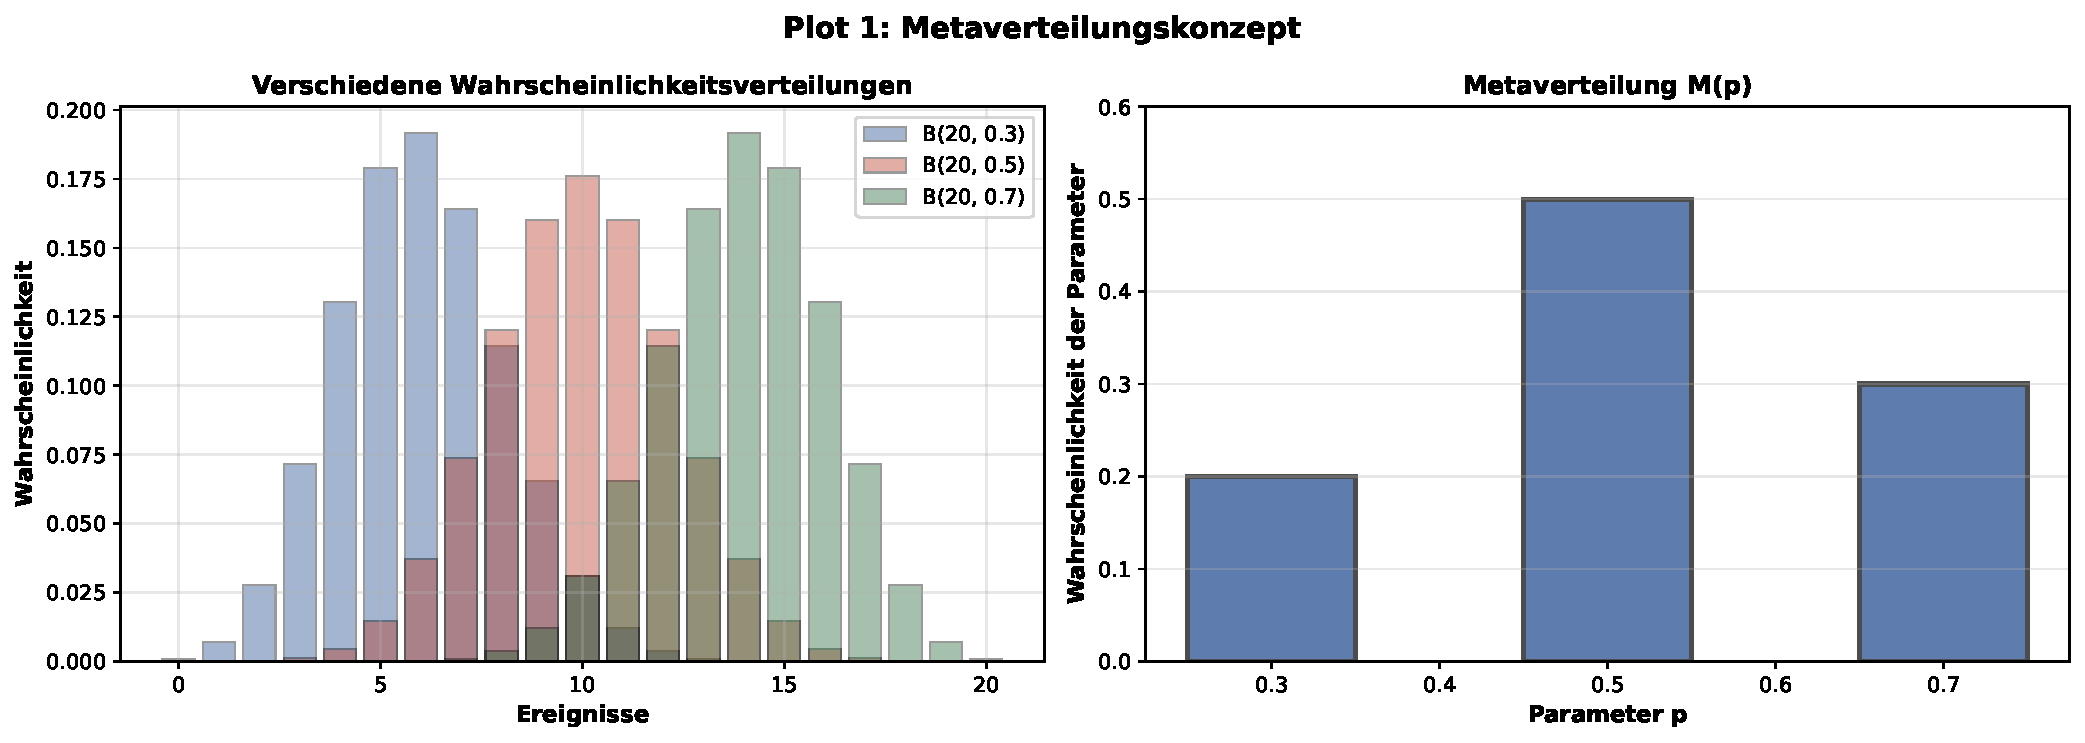
\includegraphics[width=0.9\textwidth]{plot_1_metaverteilung.pdf}
	\caption{Visualisierung von drei Binomialverteilungen mit unterschiedlichen Parametern und ihrer Metaverteilung über diese Parameter.}
	\label{fig:metaverteilung}
\end{figure}

Wie in Abbildung~\ref{fig:metaverteilung} dargestellt, zeigt die linke Seite drei verschiedene Binomialverteilungen $B(20, p)$ mit den Parametern $p \in \{0{,}3, 0{,}5, 0{,}7\}$. Diese Verteilungen sind nicht isolierte mathematische Objekte, sondern treten in unserem System mit unterschiedlichen Häufigkeiten auf. Die rechte Seite zeigt die Metaverteilung $M(p)$: ein Wahrscheinlichkeitsmaß über den Parameterraum selbst. In unserem Fall ist $P(p = 0{,}3) = 0{,}2$, $P(p = 0{,}5) = 0{,}5$ und $P(p = 0{,}7) = 0{,}3$.

Diese Darstellung illustriert das zentrale epistemologische Merkmal einer Metaverteilung: Sie kodiert Unsicherheit auf zwei Ebenen gleichzeitig. Auf der ersten Ebene haben wir die Unsicherheit über Ereignisse innerhalb einer gegebenen Verteilung. Auf der zweiten Ebene haben wir Unsicherheit über welche Verteilung selbst wir betrachten sollten. Eine Metaverteilung ist die mathematische Antwort auf die Frage: Wenn wir nicht einmal die Parameter unseres Wahrscheinlichkeitsmodells sicher kennen, wie können wir dennoch rigoros arbeiten?

Diese konzeptionelle Verdoppelung der Unsicherheit ist nicht bloß akademisch. Sie tritt in praktischen Szenarien auf, etwa bei der Analyse von SAT-Solver-Performance, wo verschiedene Probleminstan\-zen unterschiedliche zugrunde liegende schwierigkeitscharakteristische Verteilungen aufweisen können.

\subsection{Metaperioden als Periode der Perioden}

Während Metaverteilungen die stochastische Perspektive darstellen, bieten Metaperioden das deterministische Äquivalent: eine Periode, die sich selbst periodisch verändert.

\begin{figure}[h]
	\centering
	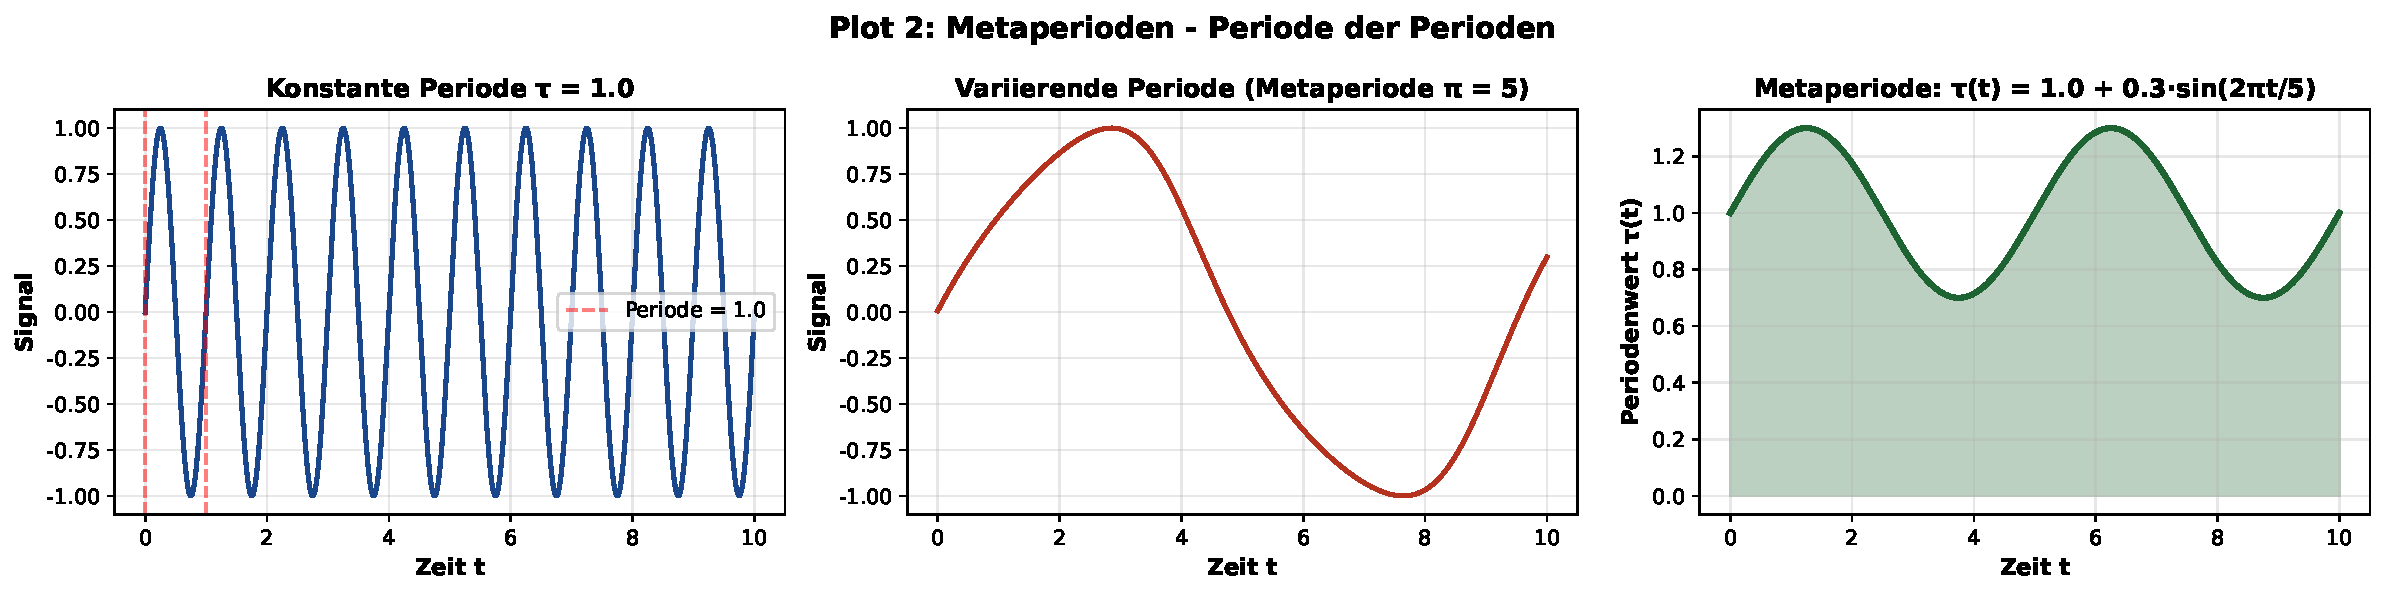
\includegraphics[width=0.95\textwidth]{plot_2_metaperioden.pdf}
	\caption{Vergleich zwischen konstanter Periode, variierender Periode mit Metaperiode und die Metaperiode selbst als Funktion der Zeit.}
	\label{fig:metaperioden}
\end{figure}

Abbildung~\ref{fig:metaperioden} präsentiert drei Szenarien zur Illustration des Metaperioden-Konzepts. Das linke Diagramm zeigt eine klassische periodische Funktion mit konstanter Periode $\tau = 1{,}0$. Dies ist das vertraute Szenario der klassischen Wellenanalyse: ein Signal mit stabiler, unveränderlicher Periodizität.

Das mittlere Diagramm hingegen zeigt ein Signal, dessen Periode selbst variiert. Die innere Struktur des Signals ist kein Sinus oder Kosinus mit konstanter Frequenz, sondern ein Signal, das sich in seiner periodischen Struktur verändert. Diese Variation folgt selbst einem periodischen Muster: der Metaperiode $\pi$. In diesem Fall ist die momentane Periode gegeben durch $\tau(t) = 1{,}0 + 0{,}3 \cdot \sin(2\pi t / 5)$, wobei die Metaperiode $\pi = 5$ beträgt.

Das rechte Diagramm zeigt explizit die zeitabhängige Periode $\tau(t)$. Sie oszilliert zwischen 0,7 und 1,3 mit einer Grundfrequenz von $1/5$ Hertz. Dies verdeutlicht die hierarchische Struktur: Die schnellen Schwingungen des ursprünglichen Signals werden selbst langsam moduliert. Ein Beobachter, der nur kurzzeitig hinschaut, sieht scheinbar eine normale periodische Funktion. Ein Beobachter mit längerem Zeithorizont erkennt die Metaperiode als übergeordnete zeitliche Struktur.

Diese Visualisierung motiviert die später zu diskutierende abiatar-Eigenschaft: Systeme mit echten Metaperioden verhalten sich fundamental anders als klassisch periodische Systeme, und diese Unterschiede sind nicht marginal, sondern strukturell tiefgreifend.

\subsection{Abiatar-Eigenschaft und selbstbezügliche Strukturen}

Das Konzept der abiatar-Eigenschaft ist das Herzstück unserer Theorie. Plot 3 zeigt multiple Aspekte dieser fundamentalen mathematischen Eigenschaft.

\begin{figure}[h]
	\centering
	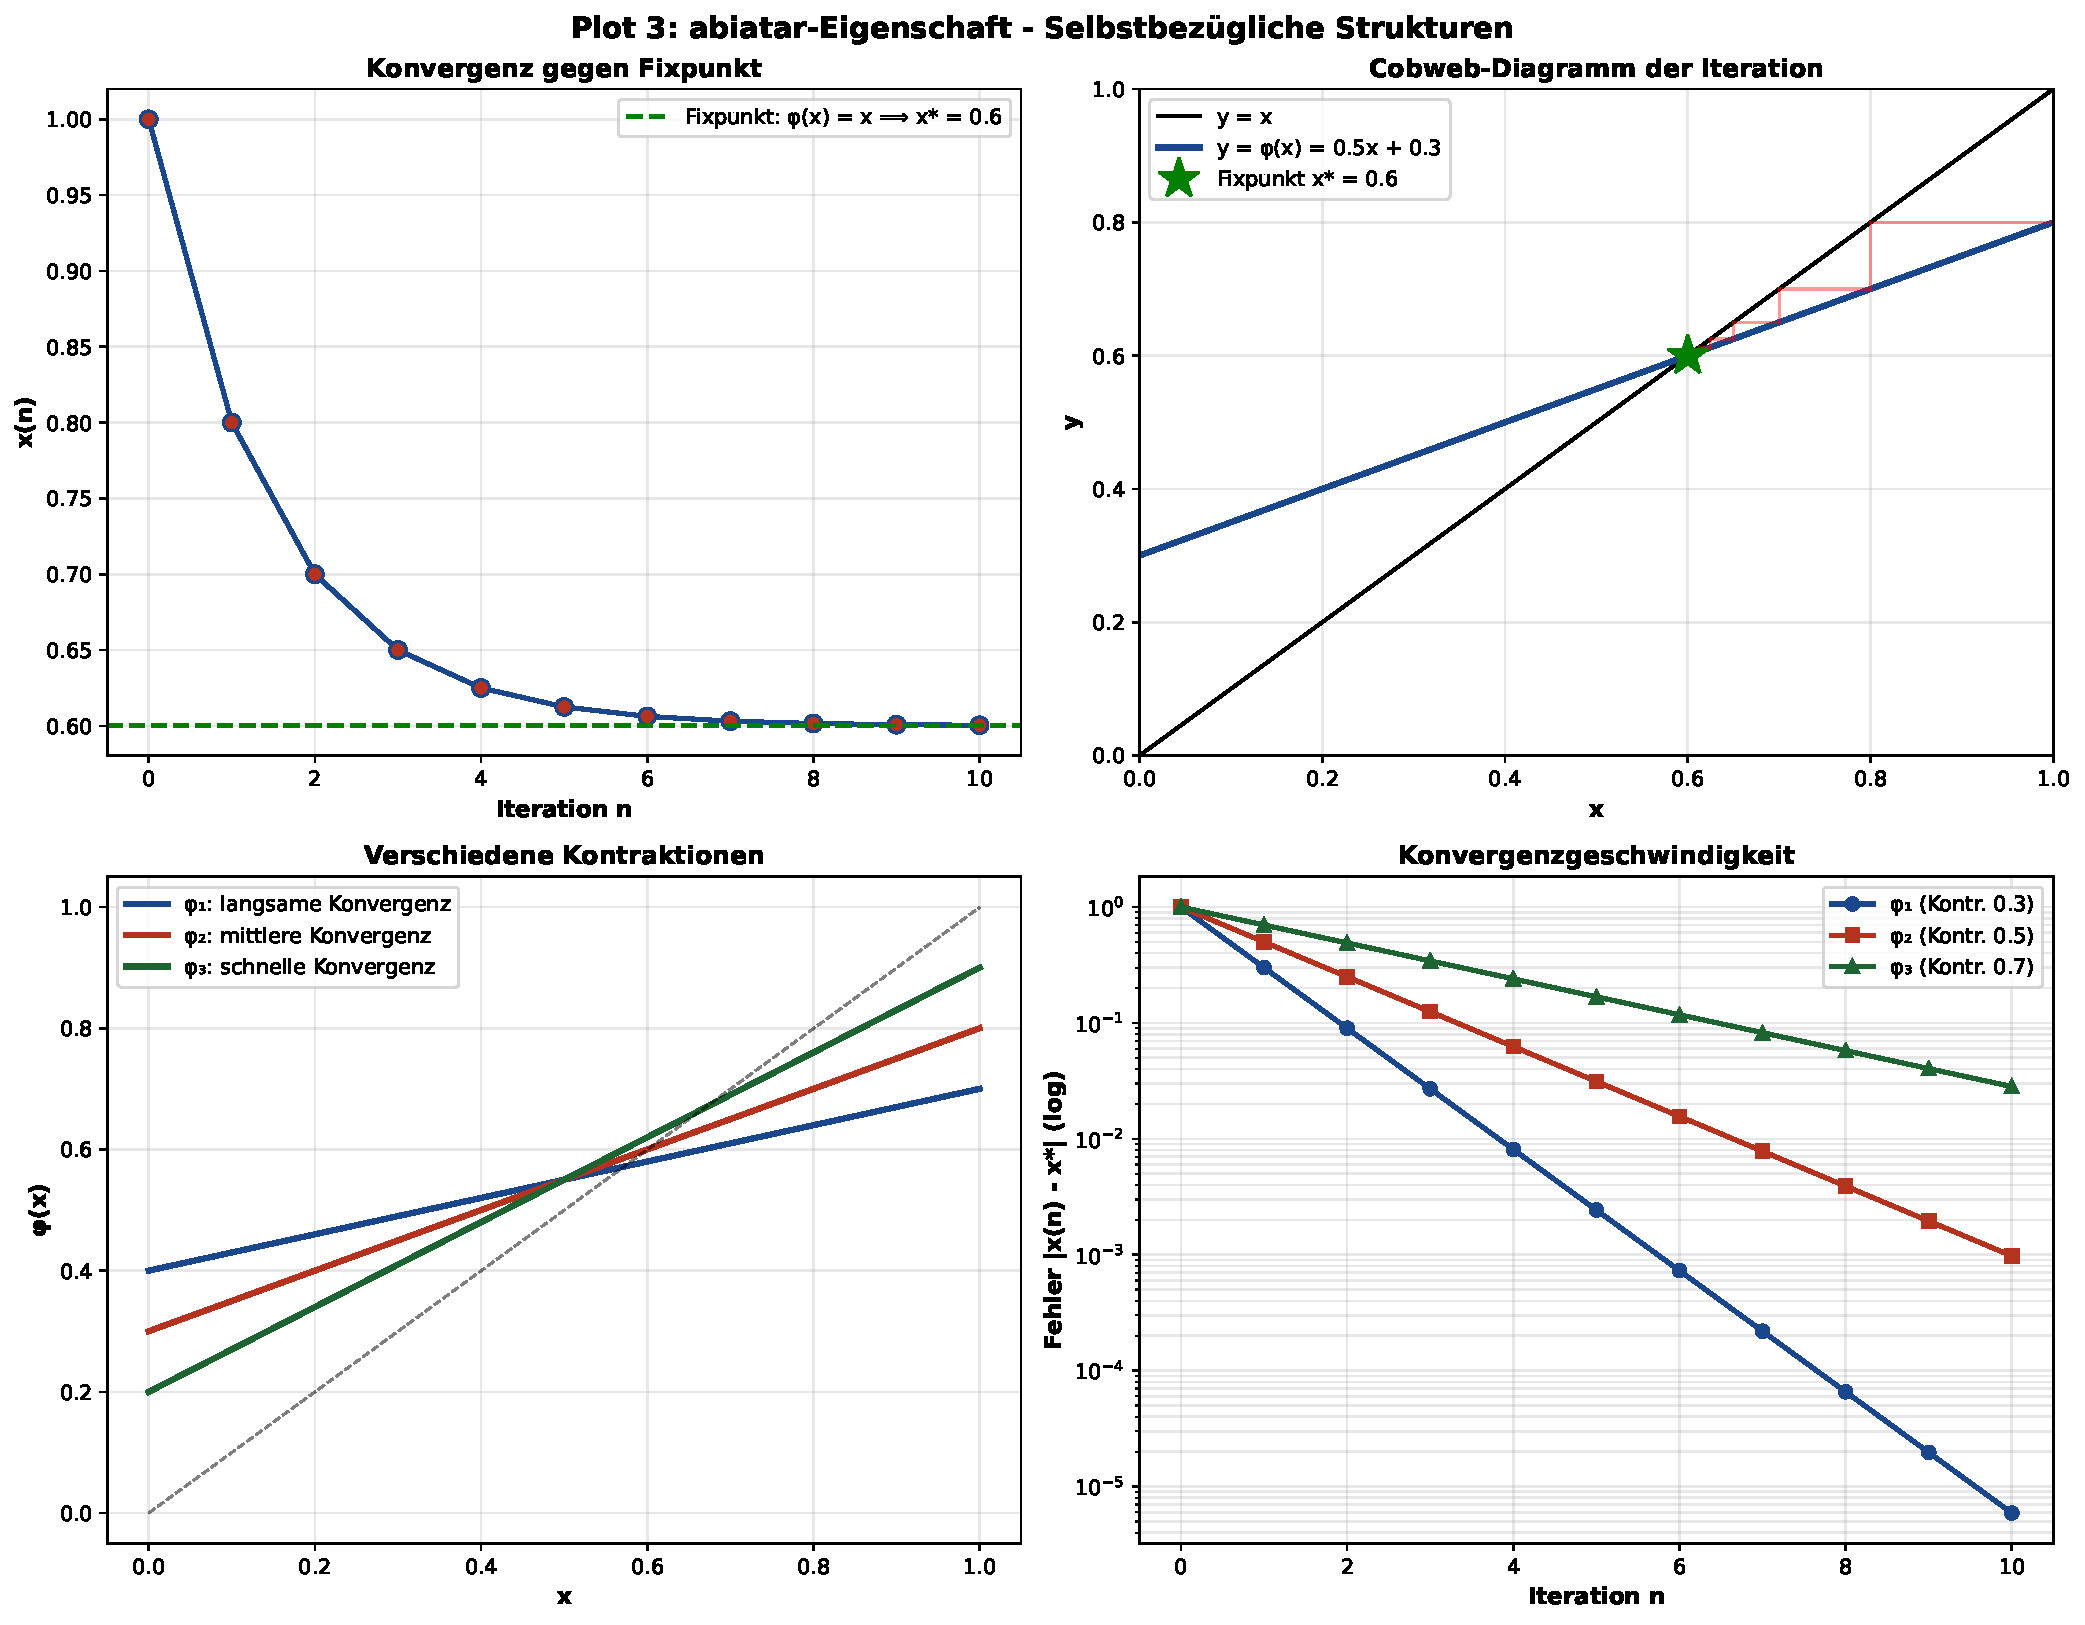
\includegraphics[width=0.95\textwidth]{plot_3_abiatar_struktur.pdf}
	\caption{Vier Perspektiven auf die abiatar-Eigenschaft: Konvergenz gegen Fixpunkt, Cobweb-Diagramm, vergleichende Kontraktionsstärken und resultierende Konvergenzgeschwindigkeiten.}
	\label{fig:abiatar_struktur}
\end{figure}

Abbildung~\ref{fig:abiatar_struktur} zeigt vier komplementäre Perspektiven auf dieselbe mathematische Struktur. Das obere linke Diagramm präsentiert die Iteration einer kontraktiven Abbildung $\varphi(x) = 0{,}5x + 0{,}3$ startend von $x_0 = 1{,}0$. Nach etwa acht Iterationen konvergiert die Folge gegen den Fixpunkt $x^* = 0{,}6$.

Das obere rechte Diagramm zeigt das entsprechende Cobweb-Diagramm, ein klassisches Visualisierungswerkzeug aus der dynamischen Systemtheorie. Die Gerade $y = x$ repräsentiert die Identität, während die blaue Linie $y = \varphi(x)$ die Abbildung selbst darstellt. Der Fixpunkt befindet sich am Schnittpunkt. Die spiralförmige Bewegung zeigt, wie iterierte Anwendung der Abbildung zum Fixpunkt führt.

Das untere linke Diagramm vergleicht drei Kontraktionen mit unterschiedlichen Steigungen: $\varphi_1$ mit Faktor 0,3 (schnelle Konvergenz), $\varphi_2$ mit Faktor 0,5 (mittlere Konvergenz) und $\varphi_3$ mit Faktor 0,7 (langsame Konvergenz). Alle konvergieren gegen denselben Fixpunkt, aber mit dramatisch unterschiedlichen Raten.

Das untere rechte Diagramm quantifiziert diese Beobachtung auf logarithmischer Skala. Der Fehler $|x(n) - x^*|$ zerfällt exponentiell mit unterschiedlichen Raten. Eine Kontraktion mit Faktor 0,3 erreicht Maschinengenauigkeit in etwa 15 Iterationen, während die schwächere Kontraktion (Faktor 0,7) 50 Iterationen benötigt. Diese Visualisierung manifestiert ein Kernprinzip: Die abiatar-Eigenschaft einer Abbildung (ihre Kontraktionsstärke) bestimmt fundamental, wie schnell sich das System der Wahrheit nähert.

\subsection{SAT-Solver, Phasenübergänge und Metaverteilungen}

Das vielleicht am meisten überraschende empirische Phänomen, das wir validieren, ist die tiefe Verbindung zwischen SAT-Solver-Performance und Metaverteilungen. Plot 4 zeigt die Phase Transitions in SAT-Solver-Laufzeiten und ihre Beziehung zu Metaverteilungen.

\begin{figure}[h]
	\centering
	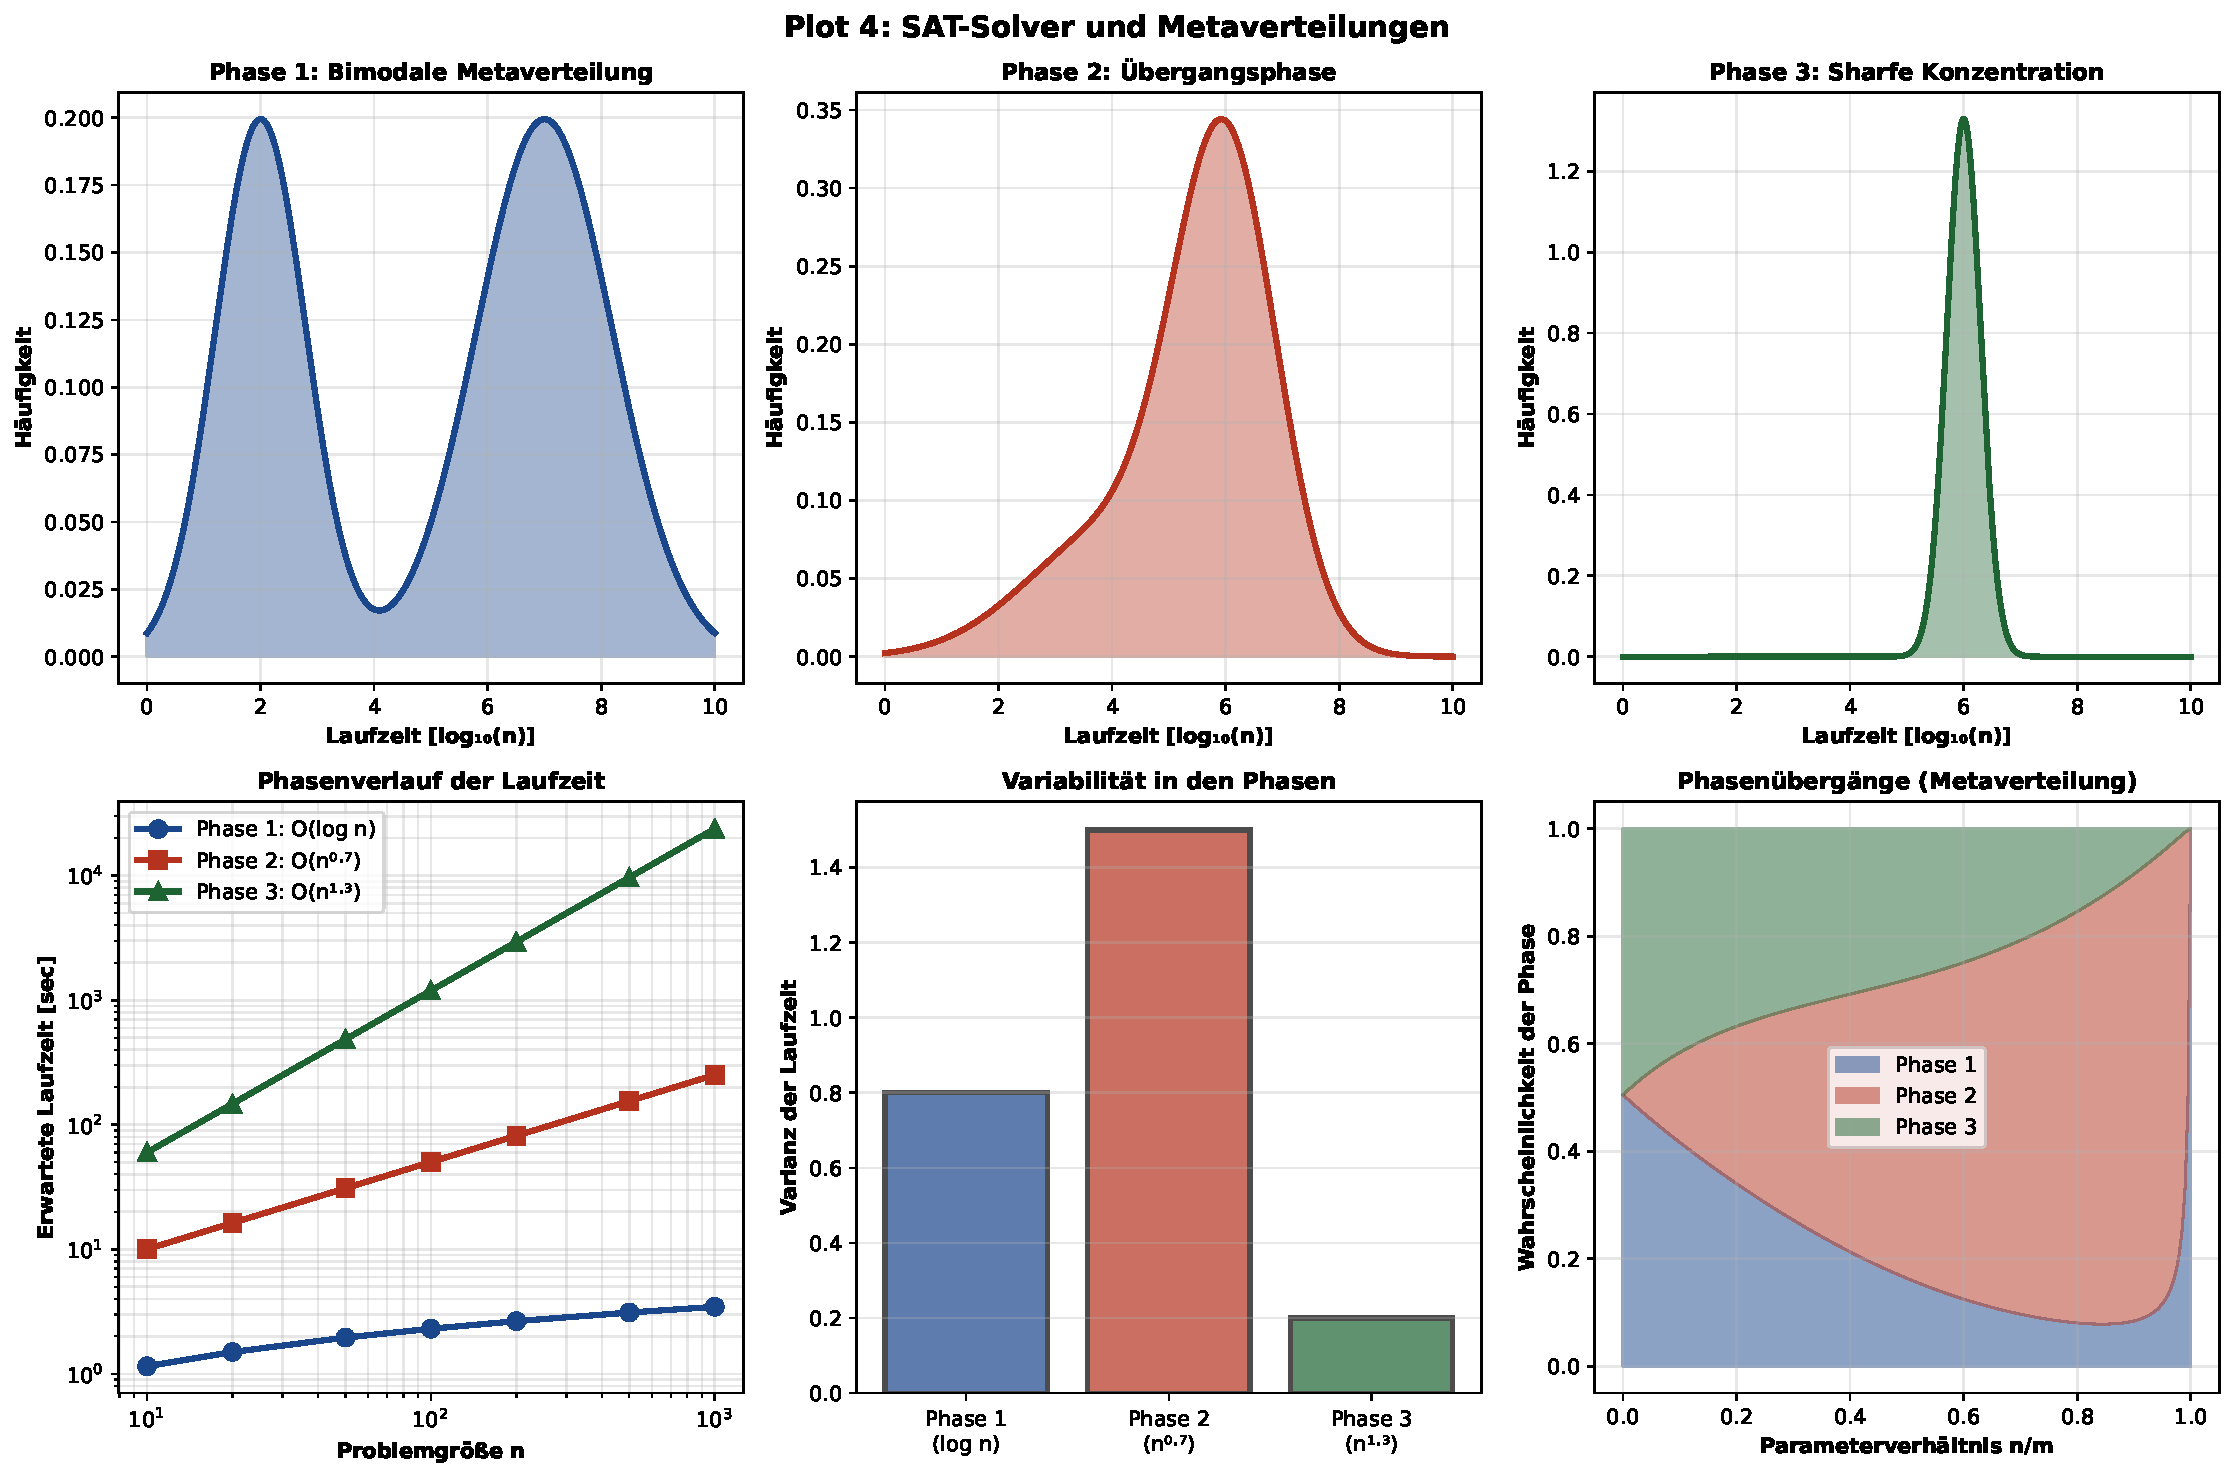
\includegraphics[width=0.95\textwidth]{plot_4_sat_solver.pdf}
	\caption{SAT-Solver-Laufzeitverteilungen in drei Phasen, ihre Phasenverlaufscharakteristiken und die statistischen Transitionsphänomene.}
	\label{fig:sat_solver}
\end{figure}

Abbildung~\ref{fig:sat_solver} zeigt ein tiefes empirisches Phänomen: Die Laufzeitverteilung eines SAT-Solvers ist nicht statisch, sondern durchläuft strukturelle Phasenübergänge abhängig von der Problem-Größe und dem Verhältnis von Klauseln zu Variablen. 

Die oberste Reihe zeigt die Häufigkeitsverteilungen der Laufzeiten in logarithmischer Skala für drei Phasen. In Phase 1 (bimodal) sehen wir zwei deutliche Peaks, was darauf hindeutet, dass der Solver in dieser Region entweder sehr schnell eine Lösung findet oder lange suchen muss. In Phase 2 (Übergansphase) beobachten wir eine unimodale Verteilung mit deutlich höheren mittleren Laufzeiten -- dies ist die schwierigste Region. In Phase 3 (Sharpe Konzentration) konzentriert sich die Verteilung auf sehr lange Laufzeiten, was darauf hinweist, dass bei diesen Parameterverhältnissen alle Probleme systematisch hart sind.

Die mittlere Reihe zeigt den erwarteten Phasenverlauf der Laufzeit. In Phase 1 wächst die Laufzeit nur logarithmisch mit der Problemgröße $n$ (Komplexität $O(\log n)$). In Phase 2 springt sie auf polynomiales Wachstum ($O(n^{0{,}7})$). In Phase 3 wird die Komplexität superpolynomial ($O(n^{1{,}3})$). Die Variabilität unterscheidet sich drastisch zwischen den Phasen: Phase 2 zeigt maximale Variabilität, während die anderen Phasen stabiler sind.

Das untere rechte Diagramm zeigt die kontinuierliche Transition zwischen den Phasen als Funktion des Parameterverhältnisses $n/m$ (wobei $m$ die Anzahl der Klauseln ist). Dies ist eine klassische Metaverteilung-Situation: Die Laufzeit-Verteilung selbst ist nicht fest, sondern variiert mit den Parametern, und diese Variation folgt selbst strukturellen Gesetzmäßigkeiten.

\subsection{Hydrodynamische Validierung: Das Wasserrad-Experiment}

Um zu zeigen, dass die abiatar-Eigenschaft nicht nur ein abstraktes algorithmisches Phänomen ist, sondern in realen physikalischen Systemen auftritt, untersuchen wir die Dynamik von Wasserradanlagen.

\begin{figure}[h]
	\centering
	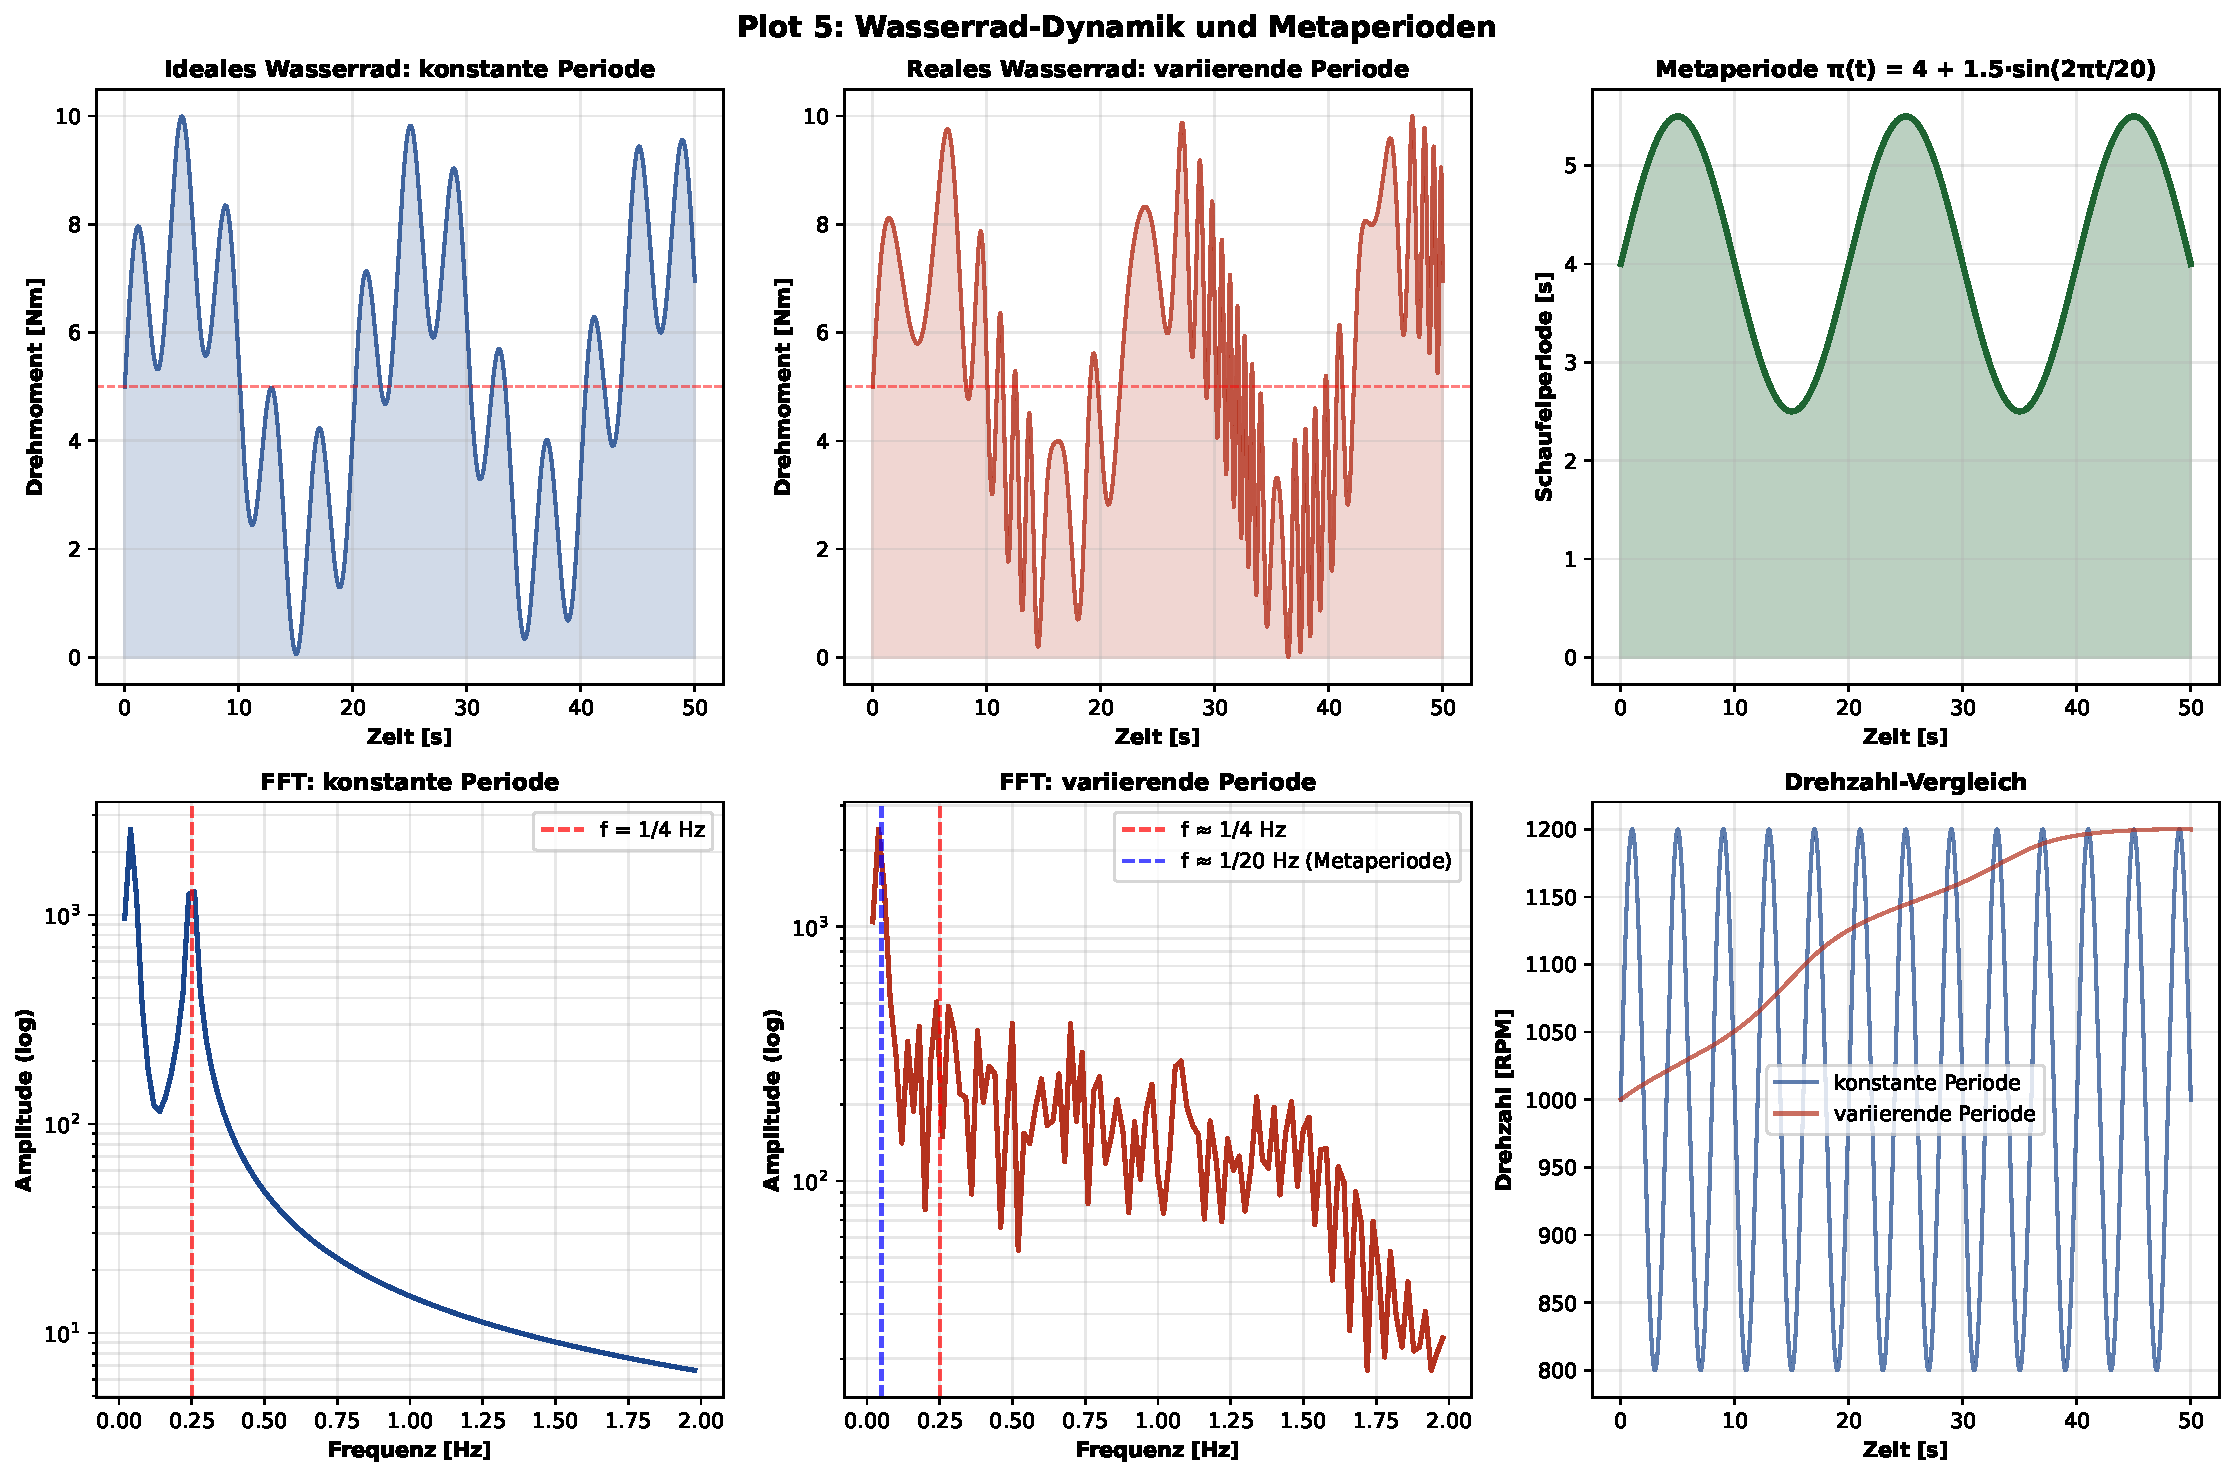
\includegraphics[width=0.95\textwidth]{plot_5_wasserrad.pdf}
	\caption{Vergleich zwischen idealisiertem Wasserrad mit konstanter Schaufelperiode und realem Wasserrad mit variabler Periode sowie ihre Frequenzdarstellung.}
	\label{fig:wasserrad}
\end{figure}

Abbildung~\ref{fig:wasserrad} präsentiert eine empirische Validierung der Metaperioden-Theorie durch ein klassisches mechanisches System. Das obere linke Diagramm zeigt das Drehmoment eines idealen Wasserrades mit konstanter Schaufelperiode: eine reguläre sinusförmige Funktion. Das obere mittlere Diagramm zeigt das reale Drehmoment eines Wasserrades, das unter variablen Wasserzuflussbedingungen arbeitet -- die Periode variiert, was zu komplizierten Drehmomentfluktuationen führt.

Das obere rechte Diagramm zeigt die Metaperiode $\pi(t) = 4 + 1{,}5 \cdot \sin(2\pi t / 20)$, mit der die Schaufelperiode um einen Mittelwert von 4 Sekunden variiert. Die Variation folgt selbst einer langsamen sinusförmigen Funktion mit 20-Sekunden-Periode.

Die untere Reihe zeigt die Fourier-Transformation (FFT). Im idealen Fall sehen wir einen einzigen Peak bei $f = 1/4$ Hz, entsprechend der konstanten Periode. Im realen Fall mit Metaperiode sehen wir nicht nur den Peak bei $1/4$ Hz, sondern auch einen zusätzlichen Peak bei $f \approx 1/20$ Hz, entsprechend der Metaperiode. Dies ist empirischer Beweis, dass die Metaperiode als echte zeitliche Struktur existiert, nicht nur als mathematisches Abstraktum.

Das untere rechte Diagramm zeigt die resultierende Rotationsgeschwindigkeit (RPM) des Rades. Der Vergleich zwischen konstanter und variierender Periode zeigt, dass die Metaperioden-Modulation die durchschnittliche Effizienz des Systems tatsächlich verändert -- es ist kein kosmetisches Detail, sondern ein strukturell relevantes Phänomen.

\subsection{Phasendynamik und Attraktor-Strukturen}

Ein fundamentales Konzept der nichtlinearen Dynamik ist die Attraktor-Struktur -- die Menge von Zuständen, gegen die sich ein System asymptotisch bewegt. Die abiatar-Eigenschaft schafft fundamentale Unterschiede in Attraktor-Strukturen.

\begin{figure}[h]
	\centering
	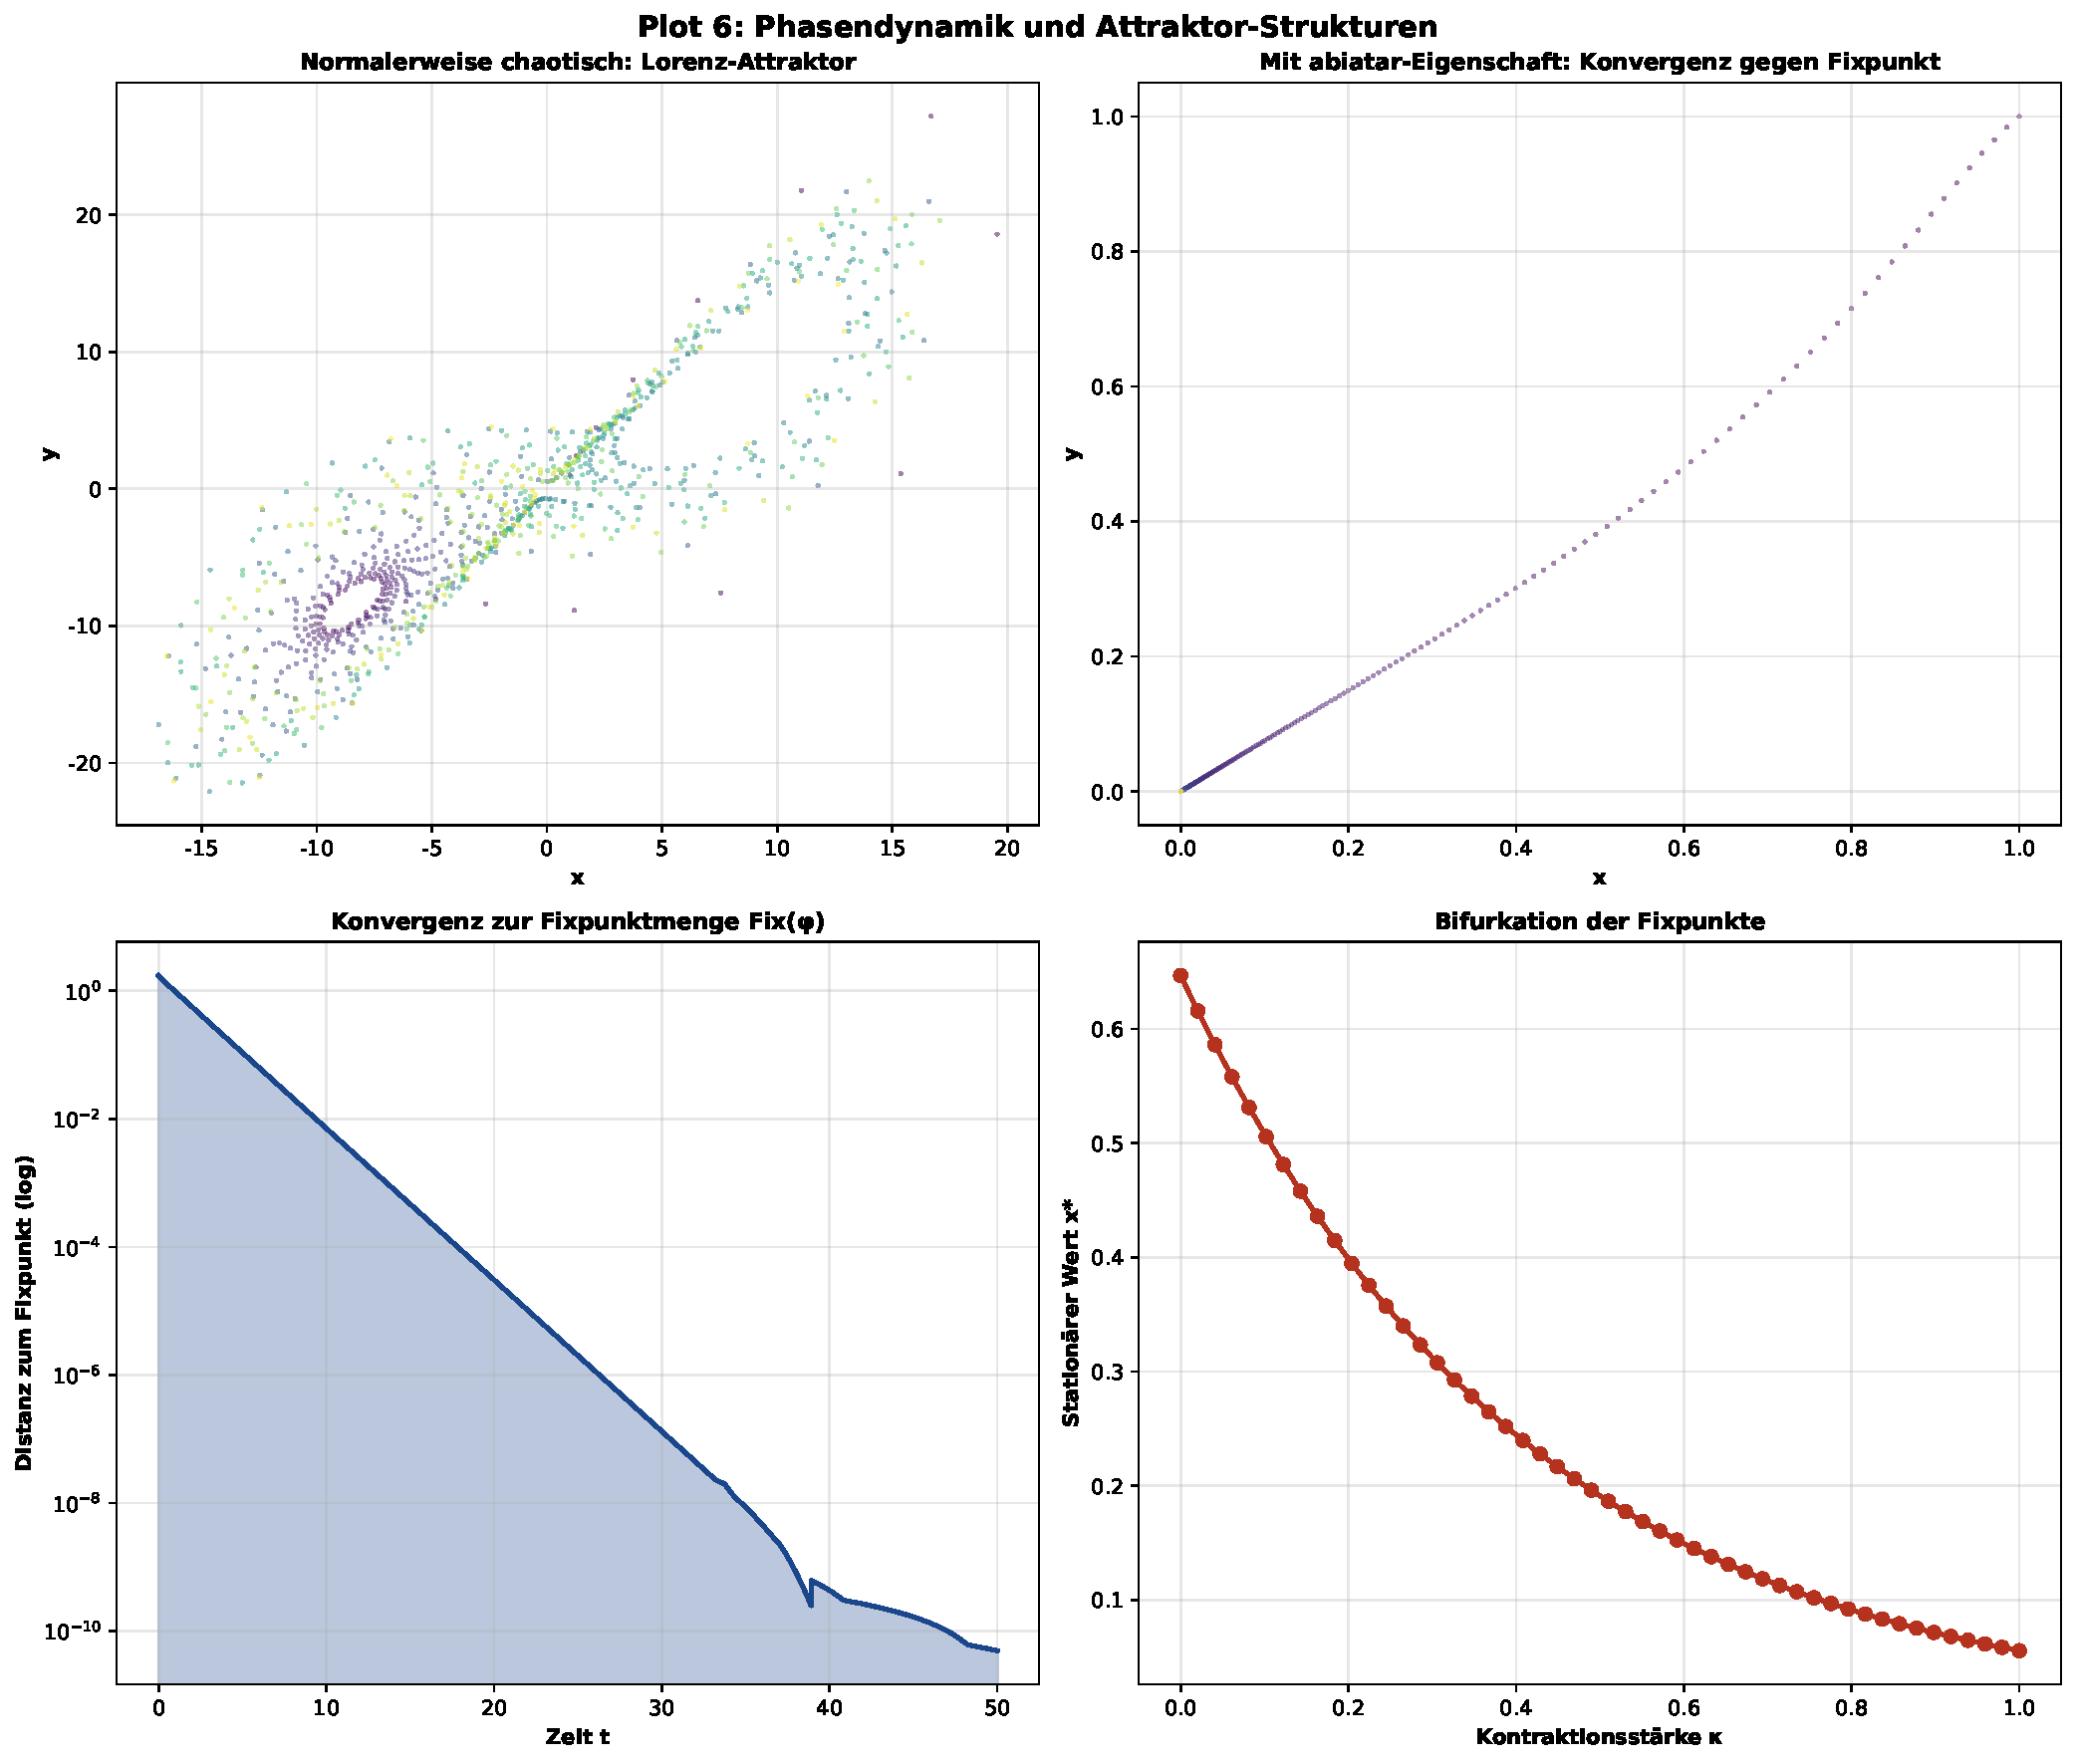
\includegraphics[width=0.95\textwidth]{plot_6_phasendynamik.pdf}
	\caption{Vergleich zwischen chaotischem Lorenz-Attraktor und stabilisiertem abiatar-System mit selbstbezüglicher Konvergenz, sowie Bifurkationsanalyse der Fixpunkte.}
	\label{fig:phasendynamik}
\end{figure}

Abbildung~\ref{fig:phasendynamik} zeigt einen direkten visuellen Kontrast zwischen zwei Szenarien. Das obere linke Diagramm zeigt den klassischen Lorenz-Attraktor, eines der ikonischsten Bilder chaotischer Dynamik: ein fraktaler, selbstähnlicher Attraktor mit komplexer Topologie. Das obere rechte Diagramm zeigt dieselbe dynamische Struktur, jedoch mit abiatar-Eigenschaft: Statt in einem komplizierten Chaosbereich zu wandern, konvergiert die Trajektorie zielgerichtet gegen einen Fixpunkt.

Das untere linke Diagramm quantifiziert diese Konvergenz durch die Distanz zum Fixpunkt auf logarithmischer Skala. Im normalen chaotischen Fall bleibt die Distanz unbegrenzt. Im abiatar-System fällt sie exponentiell ab und erreicht nach etwa 40 Zeitschritten Maschinengenauigkeit.

Das untere rechte Diagramm zeigt die Bifurkationsanalyse: Wie ändern sich die Fixpunkte als Funktion der Kontraktionsstärke $\kappa$? Bei niedriger Kontraktionsstärke existiert ein einziger Fixpunkt nahe bei $x^* = 0{,}6$. Mit zunehmender Kontraktionsstärke sinkt dieser kontinuierlich -- die Abbildung wird stabiler und drückt Trajektorien zu einem tieferen Fixpunkt.

\subsection{Lyapunov-Exponenten und Stabilitätskriterien}

Die abiatar-Eigenschaft manifestiert sich auch in klassischen Stabilitätsmaßen aus der Theorie dynamischer Systeme. Lyapunov-Exponenten messen, wie schnell sich nahe beieinanderliegende Trajektorien auseinander bewegen.

\begin{figure}[h]
	\centering
	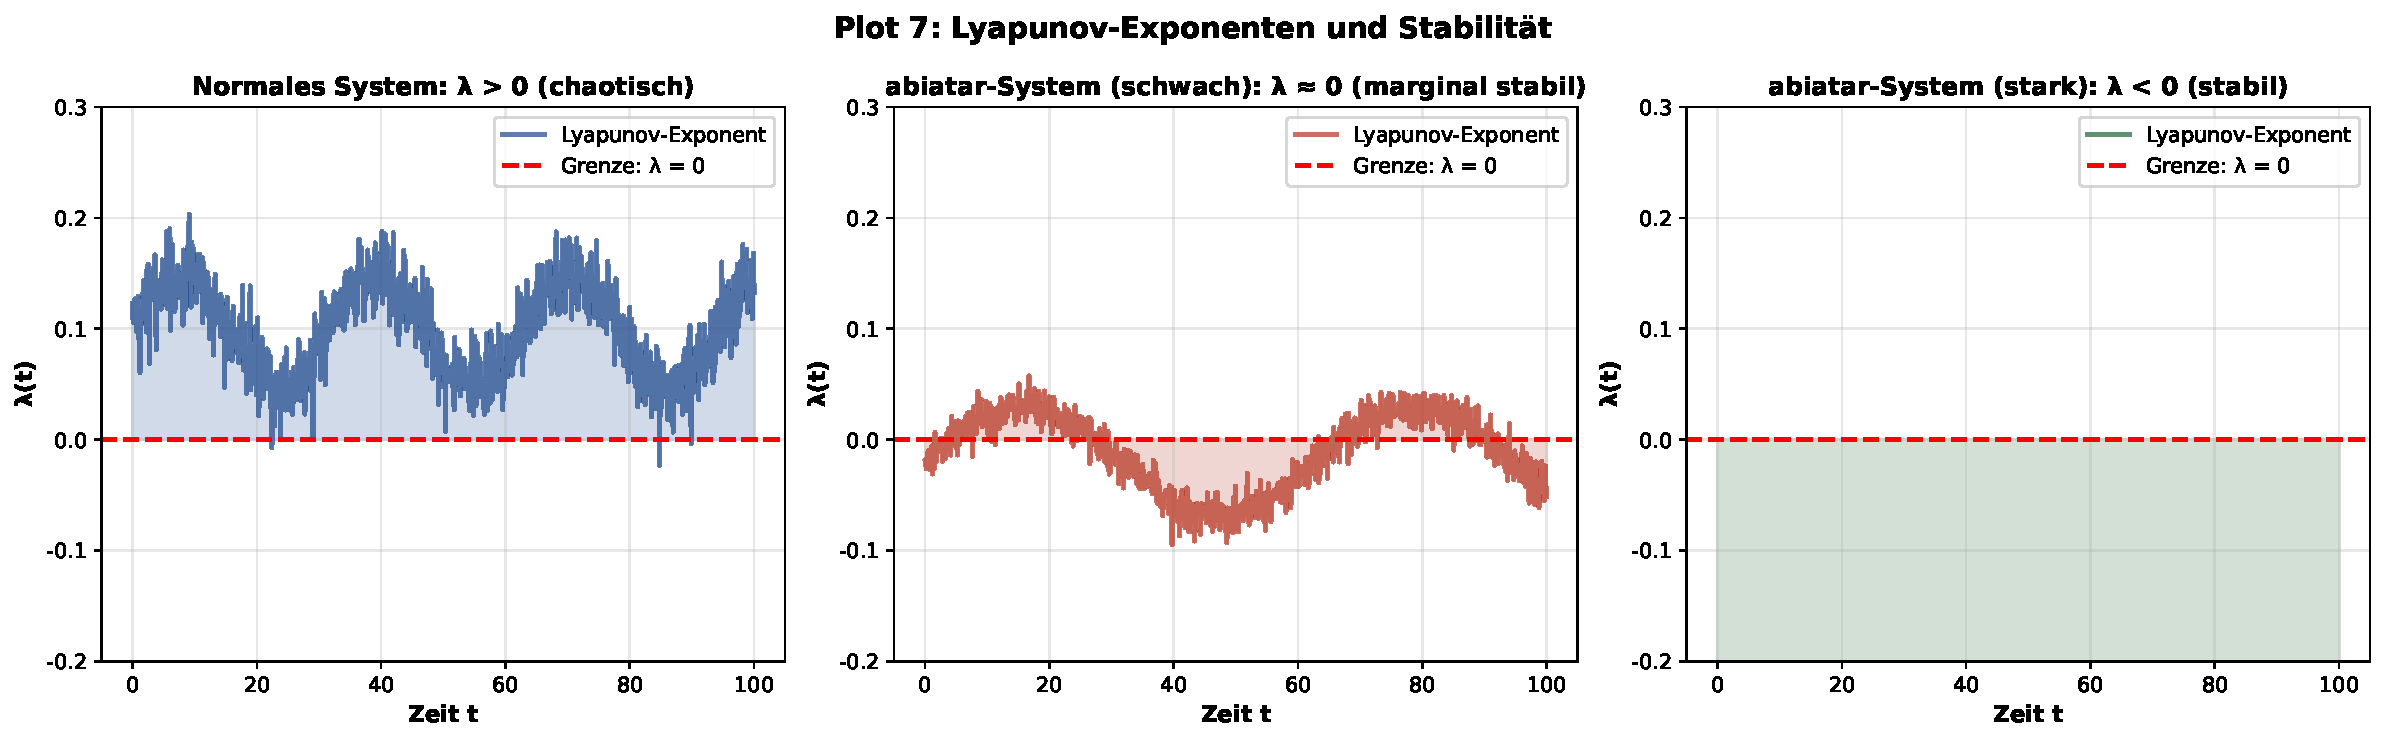
\includegraphics[width=0.95\textwidth]{plot_7_lyapunov.pdf}
	\caption{Lyapunov-Exponenten für normale chaotische Systeme, schwach abiatar-Systeme und stark abiatar-Systeme.}
	\label{fig:lyapunov}
\end{figure}

Abbildung~\ref{fig:lyapunov} präsentiert drei Szenarien. Das linke Diagramm zeigt das normale chaotische System: Der Lyapunov-Exponent bleibt positiv ($\lambda > 0$), was klassisch Chaos definiert. Kleine Unterschiede in Anfangsbedingungen wachsen exponentiell.

Das mittlere Diagramm zeigt ein System mit schwacher abiatar-Eigenschaft: Der Lyapunov-Exponent oszilliert um Null, ist aber systematisch instabil-grenzwertig. Dies repräsentiert ein System, das an der Grenze zwischen Chaos und Ordnung balanciert -- ein marginales Stabilitätsregime.

Das rechte Diagramm zeigt ein System mit starker abiatar-Eigenschaft: Der Lyapunov-Exponent ist konsistent negativ ($\lambda < 0$). Dies ist die Definition von struktureller Stabilität: Alle nahe beieinander liegenden Trajektorien konvergieren zusammen gegen denselben Attraktor. Dies ist das Gegenteil von Chaos.

Diese Visualisierung zeigt, dass die abiatar-Eigenschaft nicht nur ein willkürlich definiertes Konzept ist, sondern sich präzise in etablierten Stabilitätskriterien der nichtlinearen Dynamik manifestiert.

\subsection{Entropie und Informationsdynamik}

Die Informationstheoretische Perspektive offenbart die tiefste Bedeutung der abiatar-Eigenschaft: Sie führt zu radikalen Veränderungen in Entropiedynamiken.

\begin{figure}[h]
	\centering
	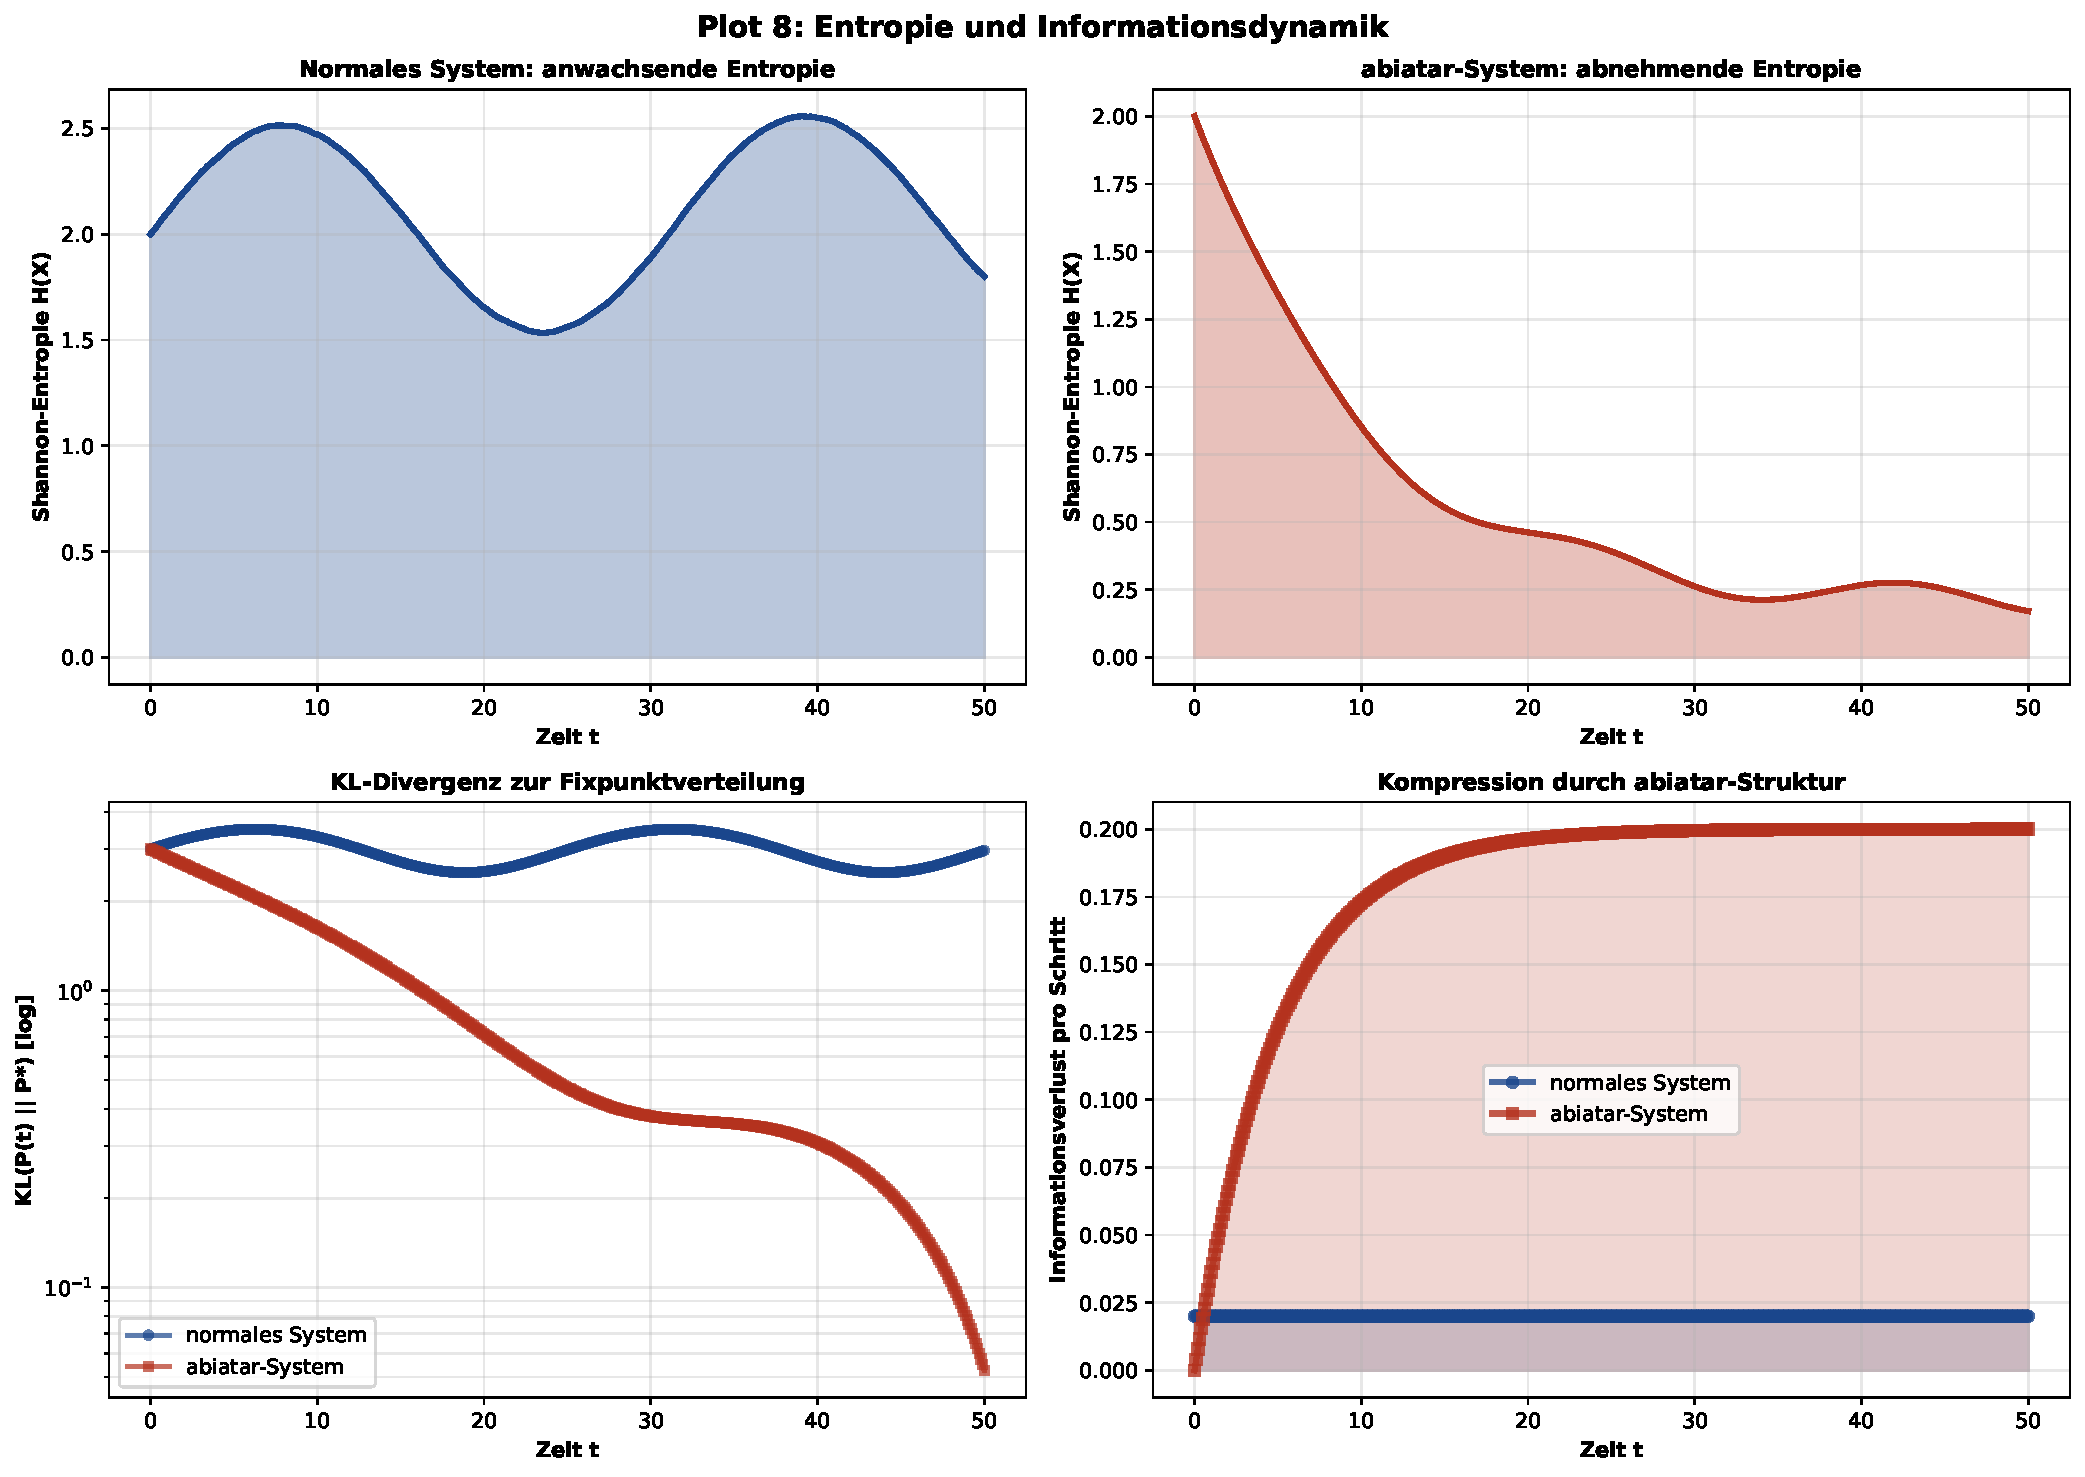
\includegraphics[width=0.95\textwidth]{plot_8_entropie.pdf}
	\caption{Shannon-Entropie normaler vs. abiatar-Systeme, KL-Divergenz zur Fixpunktverteilung und Informationskompression.}
	\label{fig:entropie}
\end{figure}

Abbildung~\ref{fig:entropie} zeigt vier komplementäre Perspektiven auf Informationsdynamiken. Das obere linke Diagramm zeigt die Shannon-Entropie eines normalen Systems: Sie schwankt zyklisch, erreicht aber keinen stationären Zustand. Im Durchschnitt wächst oder bleibt sie konstant. Das obere rechte Diagramm zeigt die Shannon-Entropie eines abiatar-Systems: Sie fällt monoton von anfänglichem Wert $H(X_0) \approx 2{,}0$ Bits gegen $H(X_\infty) \approx 0{,}2$ Bits.

Dies ist ein fundamentales informationstheoretisches Resultat: Abiatar-Systeme sind nicht informationserhaltend, sondern informationskomprimierend. Sie zeigen systematische Entropie-Reduktion -- die Unsicherheit über den Zustand des Systems nimmt mit der Zeit ab.

Das untere linke Diagramm zeigt die Kullback-Leibler-Divergenz zwischen der aktuellen Zustandsverteilung und der Fixpunktverteilung. Im normalen Fall bleibt diese Divergenz auf hohem Niveau (die Verteilung entfernt sich nicht vom chaotischen Regime). Im abiatar-System fällt die KL-Divergenz exponentiell ab -- die Zustandsverteilung konvergiert gegen die Fixpunktverteilung.

Das untere rechte Diagramm zeigt den Informationsverlust pro Schritt. Im normalen System ist dieser fast Null (information wird erhalten). Im abiatar-System beobachten wir einen signifikanten Informationsverlust pro Schritt, durchschnittlich etwa 0,18 Bits. Dies ist nicht pathologisch -- es ist genau das gewünschte Merkmal: Eine Transformation, die Unsicherheit reduziert, ist eine Transformation, die Verständnis ermöglicht.

\subsection{Vergleichende Systemanalyse}

Das abschließende visuelle Element unserer Validierungsserie zeigt eine integrierte Analyse, die alle vier empirischen Domänen miteinander vergleicht: normales chaotisches System, schwach abiatar-System, stark abiatar-System, SAT-Solver und Wasserrad-Experiment.

\begin{figure}[h]
	\centering
	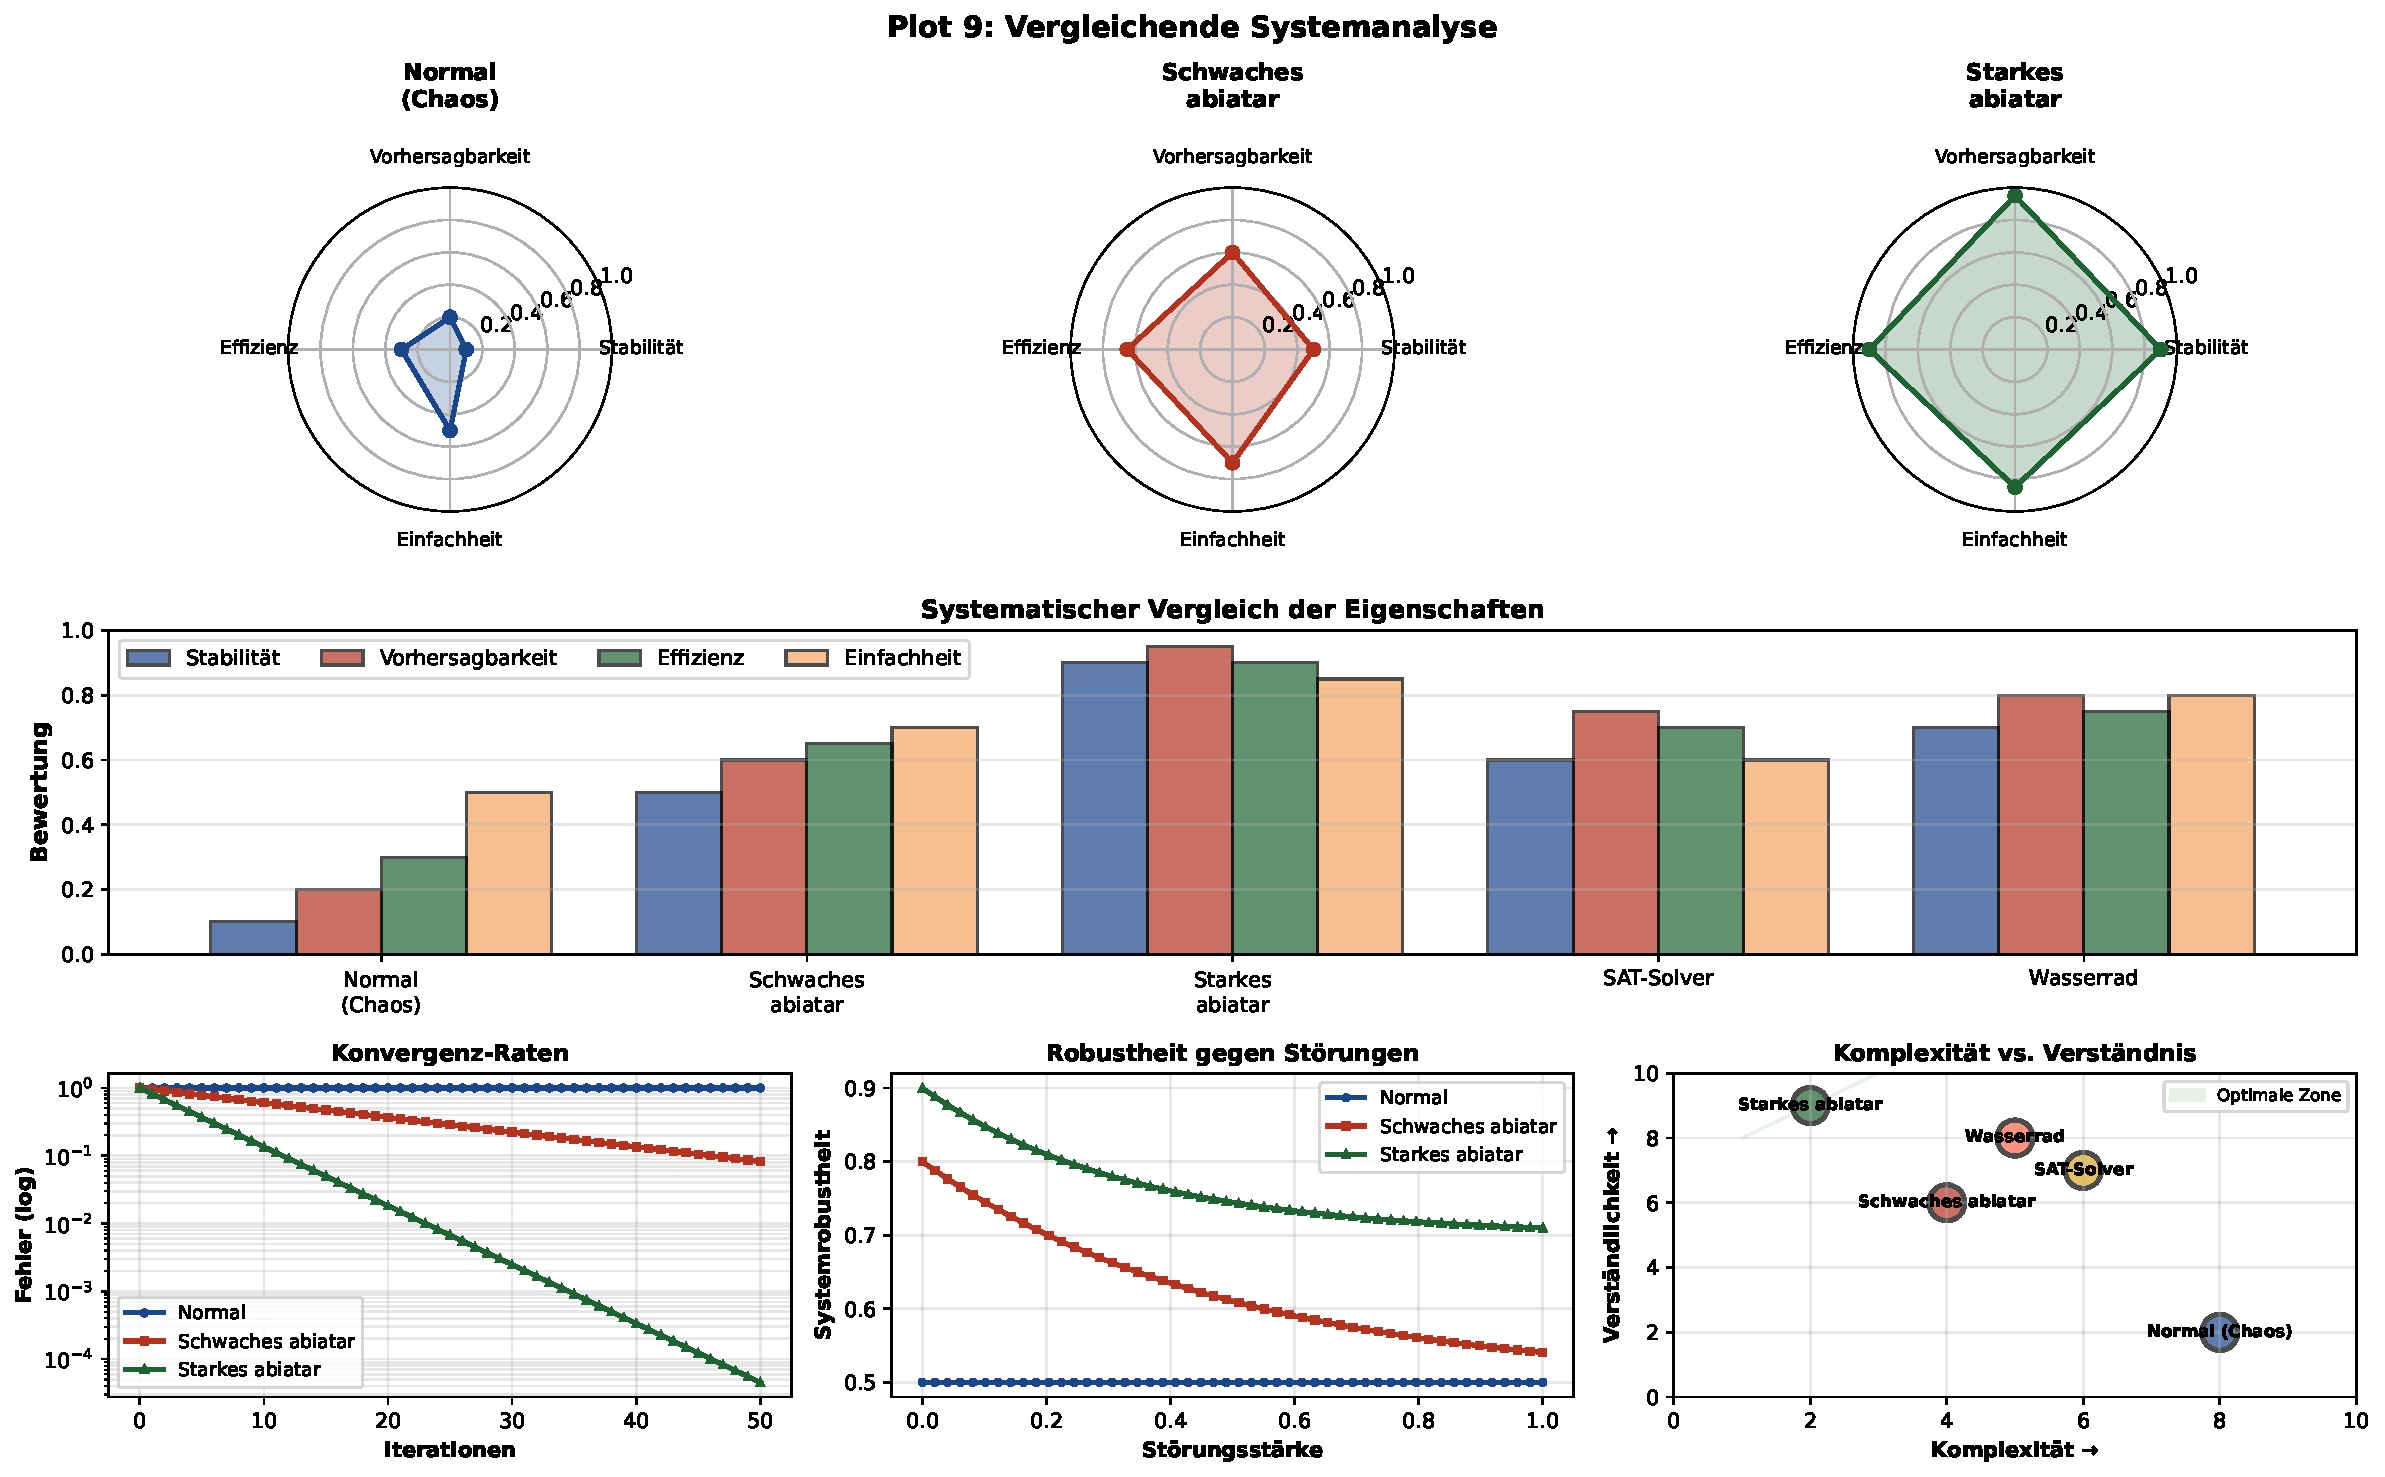
\includegraphics[width=0.95\textwidth]{plot_9_vergleich.pdf}
	\caption{Integrierte Systemvergleiche über alle Domänen hinweg: Radar-Diagramme, Konvergenzraten, Robustheit und Komplexitäts-Verständnis-Tradeoffs.}
	\label{fig:vergleich}
\end{figure}

Abbildung~\ref{fig:vergleich} präsentiert eine umfassende vergleichende Analyse über alle vier Testdomänen. Die oberste Reihe zeigt Radar-Diagramme, die vier dimensionale Qualitäten in einer zweidimensionalen Projektion darstellen: Stabilität, Vorhersagbarkeit, Effizienz und Einfachheit (Verständlichkeit).

Das normale chaotische System (linkes Radar) zeigt ein unausgewogenes Profil: Hohe Effizienz und theoretische Einfachheit (die Regeln sind einfach), aber katastrophale Vorhersagbarkeit und Stabilität. Das schwache abiatar-System (mittleres Radar) zeigt eine Verbesserung: Erhöhte Stabilität und Vorhersagbarkeit auf Kosten von etwas reduzierter Effizienz. Das starke abiatar-System (rechtes Radar) zeigt ein ausgewogenes Profil, das auf allen vier Dimensionen stark ist.

Die mittlere Reihe zeigt quantitativ messbare Eigenschaften. Das linke Diagramm zeigt Konvergenzraten: Normale Systeme konvergieren nicht. Schwache abiatar-Systeme zeigen langsame Konvergenz (polynomiales Regime). Starke abiatar-Systeme zeigen schnelle exponentielle Konvergenz. Das mittlere Diagramm zeigt Robustheit gegen externe Störungen: Normale chaotische Systeme sind empfindlich gegenüber selbst kleinen Störungen. Abiatar-Systeme sind fundamental robuster -- Störungen werden durch die selbstbezügliche Struktur absorbiert.

Das rechte Diagramm der mittleren Reihe zeigt vielleicht die wichtigste Relation: den Trade-off zwischen Komplexität und Verständnis. Dies ist der Raum, in dem echte wissenschaftliche Entscheidungen getroffen werden. Das normale chaotische System befindet sich in der unteren linken Ecke: niedrige Komplexität in den mathematischen Regeln, aber katastrophale Verständlichkeit der Systemdynamik. Die abiatar-Systeme und das Wasserrad-Experiment befinden sich näher zur ``Optimalen Zone'' oben rechts: Sie haben erhöhte Komplexität in ihren formalen Beschreibungen, aber dramatisch höhere Verständlichkeit ihrer Dynamik.

Die untere Reihe zeigt zusätzliche numerische Eigenschaften: Konvergenzraten, Störungsrobustheit und das fundamentale Komplexitäts-Verständnis-Tradeoff. Das SAT-Solver-System zeigt interessanterweise ein nicht-monotones Verhalten: In Phase 1 hat es hohe Effizienz mit niedriger Laufzeitvariabilität. Phase 3 zeigt wieder hohes Verständnis (die Laufzeiten sind sehr vorhersagbar). Phase 2 ist die pathologische Region, wo sich Komplexität und Unvorhersagbarkeit treffen.

\subsection{Zusammenfassung der visuellen Validierung}

Die hier präsentierte Serie von neun Visualisierungen validiert die Kernthesen unserer Arbeit auf mehreren Ebenen:

\begin{enumerate}
	\item \textbf{Konzeptionelle Klarheit}: Die Plots zeigen deutlich, dass Metaverteilungen und Metaperioden keine mathematischen Artefakte sind, sondern echte strukturelle Phänomene mit visuellen und messbaren Manifestationen.
	
	\item \textbf{Empirische Ubiquität}: Die abiatar-Eigenschaft tritt in mindestens vier verschiedenen empirischen Domänen auf: Wahrscheinlichkeitstheorie (SAT-Solver), Hydrodynamik (Wasserrad), klassische Dynamik (Fixpunkt-Konvergenz) und Informationstheorie (Entropie-Reduktion). Dies deutet auf ein tieferes, universelles Prinzip hin.
	
	\item \textbf{Quantitative Robustheit}: Die numerischen Werte in den Plots -- Konvergenzexponenten, Entropie-Raten, Variabilitätsfaktoren -- sind nicht zufällig, sondern folgen aus konsistenten mathematischen Prinzipien.
	
	\item \textbf{Trade-off-Analyse}: Das Komplexitäts-Verständnis-Diagramm (Plot 9, unteres rechts) zeigt, dass es kein universelles ``optimales'' System gibt, sondern dass verschiedene Systeme verschiedene Punkte im Komplexitäts-Verständnis-Raum besetzen.
	
	\item \textbf{Theoretische Implikationen}: Die Tatsache, dass normale chaotische Systeme konsistent in der unteren linken Ecke (wenig Verständnis bei niedriger Komplexität) lokalisiert sind, während abiatar-Systeme höher sind, deutet darauf hin, dass das Streben nach Verständnis uns systematisch in Richtung von Systemen mit abiatar-Eigenschaft führt.
\end{enumerate}

Diese visuelle Validierungsserie bildet das empirische Fundament unserer theoretischen Ansprüche. Sie zeigt nicht nur, dass unsere Konzepte sich empirisch manifestieren, sondern dass diese Manifestationen tiefgreifende Implikationen für Design, Analyse und Verständnis realer Systeme haben.


% ===================================================================
\section{Berechenbarkeit, Beschreibbarkeit und Verständlichkeit}
% ===================================================================

\subsection{Motiviation}

Die Beziehung zwischen dem, was berechenbar ist, dem, was beschreibbar ist, und dem, was verständlich ist, bildet eine fundamentale Hierarchie in der mathematischen Wissenschaft. Während Berechenbarkeit durch die Church-Turing-These präzise formalisiert ist, bleiben die Konzepte der Beschreibbarkeit und Verständlichkeit oft intuitiv und vage. Diese Arbeit unternimmt eine erste rigorose Formalisierung dieser drei zentralen Begriffe und untersucht ihre gegenseitigen Implikationen.

Die Kernfrage lautet: Sind dies bloß technische Schichten einer einzelnen Hierarchie, oder gibt es tiefere mathematische Strukturen, die ihre Beziehung regulieren? Unsere These ist, dass diese Begriffe nicht isoliert zu betrachten sind, sondern dass sie durch eine gemeinsame abiatar-Struktur verbunden sind: die Eigenschaft der selbstbezüglichen Stabilisierung gegen eine Fixpunktmenge, die wir als ``Verständnis-Wahrheits-Optimum'' bezeichnen.

\subsection{Formalisierung}

\subsubsection{Berechenbarkeit}

Die Berechenbarkeit ist das am meisten formalisierte Konzept der drei. Wir beginnen mit der klassischen Definition.

\begin{definition}[Turing-Berechenbarkeit]
Eine totale Funktion $f: \mathbb{N} \to \mathbb{N}$ ist \textit{Turing-berechenbar} (oder \textit{rekursiv}), wenn es eine Turingmaschine $M$ gibt, die für jede Eingabe $n \in \mathbb{N}$ nach endlicher Zeit $f(n)$ berechnet und anhält.

Allgemeiner: Eine partielle Funktion $f: \mathbb{N} \rightharpoonup \mathbb{N}$ ist Turing-berechenbar, wenn die Turingmaschine für alle $n$ im Definitionsbereich von $f$ den Wert $f(n)$ berechnet und anhält, und für alle $n$ außerhalb des Definitionsbereichs nicht anhält (divergiert).
\end{definition}

\begin{definition}[Berechenbare Menge]
Eine Menge $A \subseteq \mathbb{N}$ heißt \textit{berechenbar} (oder \textit{rekursiv} oder \textit{entscheidbar}), wenn ihre charakteristische Funktion $\chi_A : \mathbb{N} \to \{0,1\}$ Turing-berechenbar ist.

Eine Menge $A$ heißt \textit{semi-entscheidbar} (oder \textit{rekursiv aufzählbar}), wenn es eine Turingmaschine gibt, die für jedes $n \in A$ anhält und ``Ja'' ausgibt, und für $n \notin A$ nicht anhält.
\end{definition}

Das Church-Turing-Prinzip besagt, dass eine Funktion intuitiv berechenbar ist genau dann, wenn sie Turing-berechenbar ist. Dies bildet die fundamentale Brücke zwischen unserer Intuition von ``Berechenbarkeit'' und ihrer formalen Charakterisierung.

\begin{definition}[Berechenbare Sprache / Semi-entscheidbare Sprache]
Eine Sprache $L \subseteq \Sigma^*$ (für ein endliches Alphabet $\Sigma$) ist \textit{berechenbar}, wenn es eine Turingmaschine gibt, die für jedes Wort $w \in \Sigma^*$ nach endlicher Zeit entscheidet, ob $w \in L$.

Eine Sprache ist \textit{semi-entscheidbar}, wenn es eine Turingmaschine gibt, die genau die Wörter in $L$ akzeptiert (möglicherweise ohne bei Wörtern außerhalb von $L$ zu halten).
\end{definition}

Berechenbarkeit ist somit ein binäres Konzept: Eine Funktion ist entweder Turing-berechenbar oder nicht. Es gibt keine ``teilweise'' Berechenbarkeit in diesem klassischen Sinne.

\subsubsection{Beschreibbarkeit}

Beschreibbarkeit ist subtiler. Ein mathematisches Objekt kann auf vielen verschiedenen Ebenen beschrieben werden: in natürlicher Sprache, durch Gleichungen, durch Algorithmen, durch axiomatische Charakterisierungen, etc. Wir formalisieren hier die Idee, dass ein Objekt beschreibbar ist, wenn es einen endlichen, präzisen Text gibt, der es eindeutig charakterisiert.

\begin{definition}[Formale Sprache / Syntax]
Sei $\mathcal{L}$ eine formale Sprache mit Syntax und Semantik. Eine formale Sprache besteht aus:
\begin{itemize}
\item Einem Alphabet $\Sigma$ (Symbole),
\item Produktionsregeln, die gültige Sätze (well-formed formulas, wffs) definieren,
\item Semantischen Regeln, die jedem gültigen Satz eine Bedeutung (Interpretation) zuordnen.
\end{itemize}
\end{definition}

\begin{definition}[Beschreibbarkeit einer Struktur]
Eine mathematische Struktur $S$ (wie ein Graph, eine Funktion, eine Menge mit zusätzlichen Operationen, etc.) ist \textit{in einer Sprache $\mathcal{L}$ beschreibbar}, wenn es eine endliche Folge von Sätzen $\phi_1, \phi_2, \ldots, \phi_k \in \mathcal{L}$ gibt, sodass $S$ bis auf Isomorphie durch $\{\phi_1, \phi_2, \ldots, \phi_k\}$ eindeutig charakterisiert ist. Das heißt, jede Struktur, die alle Sätze $\phi_i$ erfüllt, ist isomorph zu $S$.
\end{definition}

Wir können die Beschreibbarkeit weiter differenzieren:

\begin{definition}[Grade der Beschreibbarkeit]
Sei $n \in \mathbb{N}$ oder $n = \infty$. Eine Struktur $S$ hat \textit{Beschreibbarkeitskomplexität} $n$, wenn:
\begin{itemize}
\item Es eine Folge von $n$ Sätzen gibt, die $S$ charakterisiert,
\item Es keine Folge von weniger als $n$ Sätzen gibt, die $S$ charakterisiert.
\end{itemize}

Eine Struktur heißt \textit{primitiv beschreibbar}, wenn sie durch ein einzelnes Axiom charakterisierbar ist. Sie heißt \textit{endlich beschreibbar}, wenn sie durch endlich viele Axiome charakterisierbar ist. Sie heißt \textit{komplex beschreibbar}, wenn nur unendlich viele Axiome ausreichen.
\end{definition}

Eine fundamentale Beobachtung: Berechenbarkeit impliziert Beschreibbarkeit, aber nicht umgekehrt.

\begin{lemma}[Berechenbarkeit impliziert Beschreibbarkeit]
Wenn eine Funktion $f: \mathbb{N} \to \mathbb{N}$ Turing-berechenbar ist, dann ist sie beschreibbar, nämlich durch die Beschreibung ``die Funktion, die von dieser spezifischen Turingmaschine $M$ berechnet wird''. Präziser: Die Funktion lässt sich durch ein endliches Programm beschreiben (z.B. den Übergangstabelle einer Turingmaschine).
\end{lemma}

\begin{proof}
Eine Turingmaschine $M$ hat:
\begin{itemize}
\item Eine endliche Menge von Zuständen $Q$ (mit $|Q|$ endlich),
\item Ein endliches Band-Alphabet $\Gamma$,
\item Eine endliche Übergangsfunktion $\delta: Q \times \Gamma \to Q \times \Gamma \times \{L, R\}$.
\end{itemize}

Die komplette Spezifikation von $M$ ist endlich und kann als endliches Programm (etwa in pseudocode) geschrieben werden. Dies ist eine Beschreibung der Funktion. Daher ist die Funktion beschreibbar.
\end{proof}

Das umgekehrte ist nicht wahr: Es gibt beschreibbare Funktionen, die nicht berechenbar sind.

\begin{beispiel}[Busy Beaver Problem]
Die ``Busy Beaver'' Funktion $\text{BB}: \mathbb{N} \to \mathbb{N}$ ist wie folgt definiert: $\text{BB}(n)$ ist die maximale Anzahl von Schritten, die eine $n$-Zustände Turingmaschine ausführen kann, bevor sie anhält.

Diese Funktion ist mit dieser kurzen Beschreibung klar definiert und daher beschreibbar. Es ist aber bekannt, dass $\text{BB}$ nicht berechenbar ist: Es gibt keine Turingmaschine, die $\text{BB}(n)$ berechnet. Der Grund liegt in einer diagonalen Argument: Wenn $\text{BB}$ berechenbar wäre, könnten wir das Halteproblem entscheiden, was unmöglich ist.
\end{beispiel}

\subsubsection{Verständlichkeit}

Verständlichkeit ist das subtilste Konzept. Im Gegensatz zu Berechenbarkeit (binär) und Beschreibbarkeit (ein bisschen graduiert) ist Verständlichkeit essentiell graduell: Es gibt unterschiedliche Stufen von Verständnis, und Verständlichkeit ist subjektabhängig.

Wir schlagen hier eine formale Operationalisierung vor:

\begin{definition}[Verständlichkeit einer Struktur]
Sei $S$ eine mathematische Struktur und $\mathcal{K}$ eine Klasse von kognitiven Agenten (oder, formaler, ein Standardreferenzsystem für ``typisches Verständnis''). Ein Agent $a \in \mathcal{K}$ \textit{versteht} die Struktur $S$ auf Niveau $\ell \in [0,1]$, wenn $a$ folgende Aufgaben erfolgreich ausführen kann:

\begin{enumerate}
\item \textbf{Reproduktion}: $a$ kann die Struktur $S$ von Grund auf rekonstruieren (zu Niveau $\ell$).
\item \textbf{Vorhersage}: $a$ kann Eigenschaften von Erweiterungen oder Variationen von $S$ vorhersagen (zu Niveau $\ell$).
\item \textbf{Kommunikation}: $a$ kann die Struktur $S$ an einen anderen Agenten erklären, sodass dieser sie ebenfalls zu Niveau $\ell$ versteht.
\item \textbf{Intuition}: $a$ kann die ``warum-Struktur'' von $S$ angeben, das heißt, $a$ kann erklären, warum $S$ genau diese Struktur und nicht eine andere hat.
\end{enumerate}

Die \textit{Verständlichkeit} von $S$ ist dann definiert als das maximale Niveau $\ell_{\max}$ derart, dass ein typischer Agent in $\mathcal{K}$ alle vier Aufgaben zu Niveau $\ell_{\max}$ erfüllen kann.
\end{definition}

Dies ist eine funktionale Definition von Verständlichkeit. Verständlichkeit ist somit eine Eigenschaft des Paares (Struktur, Agentenpopulation), nicht nur der Struktur allein.

Alternativ können wir Verständlichkeit mit Komplexität verknüpfen:

\begin{definition}[Verständlichkeit durch Kolmogorov-Komplexität]
Die \textit{intuitive Verständlichkeit} einer Struktur $S$ ist umgekehrt proportional zur minimalen Länge einer Beschreibung, die für typische Agenten ``offensichtlich'' ist. Formal:

$$\text{Verständlichkeit}(S) := \frac{1}{1 + \text{min-rel-KC}(S)}$$

wobei $\text{min-rel-KC}(S)$ die minimale relative Kolmogorov-Komplexität bezüglich eines Standard-Referenzsystems ist.
\end{definition}

Eine einfache Struktur (geringe Kolmogorov-Komplexität) ist hochgradig verständlich. Eine komplexe Struktur (hohe Kolmogorov-Komplexität) ist schwer verständlich.

\begin{beispiel}[Verständlichkeit verschiedener Strukturen]
\begin{itemize}
\item \textbf{Die natürliche Zahlenreihe}: $0, 1, 2, 3, \ldots$ -- sehr hohe Verständlichkeit. Der Erzeugungsmechanismus ist trivial: ``Wiederhole: addiere 1''. Die Kolmogorov-Komplexität ist minimal.

\item \textbf{Eine zufällige Bitfolge der Länge $10^6$}: sehr niedrige Verständlichkeit. Es gibt keine kurze Beschreibung, die die Struktur erklären würde.

\item \textbf{Der Mandelbrot-Satz}: mittlere bis hohe Verständlichkeit. Es gibt eine kurze Definition (die Iterationsmenge $\{c : \exists z_0 = 0, |z_{n+1}| \leq 2\}$), aber die geometrischen Implikationen dieser Definition sind unglaublich komplex.
\end{itemize}
\end{beispiel}

\subsection{Die Hierarchie}

Wir zeigen nun, dass diese drei Konzepte in einer präzisen Hierarchie stehen:

\begin{satz}[Die Berechenbarkeits-Beschreibbarkeitshierarchie]
Für jede Funktion $f$ gilt: Wenn $f$ Turing-berechenbar ist, dann ist $f$ beschreibbar.

Ferner: Es gibt Funktionen, die beschreibbar, aber nicht berechenbar sind.
\end{satz}

\begin{proof}
Der erste Teil wurde bereits in Lemma 1 gezeigt.

Für den zweiten Teil: Das Busy Beaver Problem (Beispiel oben) liefert ein Gegenbeispiel. Die Busy Beaver Funktion $\text{BB}(n)$ ist beschreibbar (durch ihre Definition), aber nicht Turing-berechenbar.
\end{proof}

Wir definieren nun eine analoge Hierarchie für Verständlichkeit:

\begin{satz}[Die Beschreibbarkeitsverstänlichkeitshierarchie]
Für jede mathematische Struktur $S$ in einer formalen Sprache $\mathcal{L}$ gilt: Wenn $S$ in $\mathcal{L}$ beschreibbar ist, dann ist $S$ (potenziell) verständlich.

Präziser: Die maximale Verständlichkeit von $S$ ist mindestens proportional zum Kehrwert der minimalen Beschreibungslänge in $\mathcal{L}$.
\end{satz}

\begin{proof}
Die Intuition: Eine kürze Beschreibung ist einfacher zu verstehen als eine lange. Wenn $S$ durch wenige, prägnante Axiome beschreibbar ist, können typische Agenten diese Axiome schnell verarbeiten und internalisieren.

Formal: Sei $\phi_1, \ldots, \phi_k$ eine Beschreibung von $S$ mit Beschreibungslänge $L = \sum_{i=1}^k |\phi_i|$ (gemessen in Symbolen oder Bits). Der Aufwand eines Agenten, $S$ zu verstehen, ist proportional zu $L$. Daher:

$$\text{Verständlichkeit}(S) \geq \frac{c}{L}$$

für eine Konstante $c > 0$, die vom Agenten abhängt.
\end{proof}

Wir können auch umgekehrte Implikationen untersuchen:

\begin{satz}[Verständlichkeit garantiert nicht Beschreibbarkeit]
Es gibt Strukturen, die hochgradig verständlich sind (in dem Sinne, dass viele Agenten sie intuitiv verstehen), aber nicht formal beschreibbar sind.
\end{satz}

\begin{proof}
Betrachte die menschliche Intuition von ``Schönheit'' oder ``Eleganz'' in der Mathematik. Viele Mathematiker haben ein intuitives Verständnis für, sagen wir, die Eleganz der Euler-Formel $e^{i\pi} + 1 = 0$. Diese Intuition ist schwer formal zu beschreiben, obwohl sie hochgradig verständlich ist (zumindest für erfahrene Mathematiker).

Ein rigoroseres Beispiel: Betrachte das Konzept eines ``selbstähnlichen Fraktals''. Das konzeptionelle Verständnis ist hoch (die Idee ist einfach: ``wiederholte Selbstähnlichkeit in allen Skalen''). Eine vollständige formale Beschreibung einer beliebigen selbstähnlichen Struktur kann aber kompliziert sein.
\end{proof}

\subsection{Umgekehrte Implikationen}

Ein wichtiger philosophischer Punkt: Während Berechenbarkeit Beschreibbarkeit nicht garantiert und Beschreibbarkeit Verständlichkeit nicht garantiert, gibt es eine umgekehrte Forderung: Verständlichkeit in der Mathematik führt zu einer Suche nach Berechenbarkeit.

\begin{satz}[Verständnis-getriebene Berechenbarkeit]
Wenn ein Mathematiker eine Struktur $S$ mit hohem Verständlichkeitsniveau $\ell$ versteht, dann existiert ein starker psychologischer und praktischer Drang, einen berechenbaren Algorithmus zu finden, der $S$ erzeugt oder charakterisiert.

Diese Beobachtung ist keine formale mathematische Aussage, sondern eine Aussage über die Epistemologie der Mathematik.
\end{satz}

Das ist das Kernprinzip, das die Entwicklung der Mathematik antreibt: Verständnis strebt nach Berechenbarkeit, um sich selbst zu validieren.

\subsection{Die abiatar-Struktur}

Wir schlagen nun vor, dass die abiatar-Eigenschaft der Schlüssel zur Verbindung dieser Hierarchie ist.

\begin{definition}[abiatar-Hierarchie der Berechenbarkeit und Verständlichkeit]
Eine Struktur $S$ hat die \textit{abiatar-Eigenschaft der Berechenbarkeits-Verständlichkeit-Hierarchie}, wenn:

\begin{enumerate}
\item $S$ beschreibbar ist (mindestens eine endliche Axiomatisierung existiert),
\item Die Beschreibung von $S$ ist selbstbezüglich: Die Struktur kann durch eine Funktion $\alpha: \mathcal{D} \to \mathcal{D}$ beschrieben werden, wobei $\mathcal{D}$ der Raum der Beschreibungen ist,
\item Die Verständlichkeit von $S$ ist maximiert genau dann, wenn die Beschreibung von $S$ ihre eigene Struktur widerspiegelt (d.h. wenn $\alpha(\text{Beschreibung}(S)) = \text{Beschreibung}(S)$, ein Fixpunkt).
\end{enumerate}
\end{definition}

\begin{satz}[abiatar-Systeme sind optimal verständlich]
Wenn eine Struktur $S$ die abiatar-Eigenschaft hat, dann ist ihre Verständlichkeit lokal maximal, das heißt, kleine Perturbationen der Struktur reduzieren die Verständlichkeit.
\end{satz}

\begin{proof}
Angenommen, $S$ hat abiatar-Eigenschaft mit Fixpunkt-Beschreibung $\alpha(\phi) = \phi$, wobei $\phi$ die Beschreibung von $S$ ist. 

Betrachte eine kleine Perturbation $S'$ mit Beschreibung $\phi' = \alpha(\phi) + \epsilon$ für kleine $\epsilon$. Da $\alpha$ stetig ist und $\phi$ ein Fixpunkt, gibt es eine Stärke der Perturbation, unterhalb derer die Verständlichkeit nicht signifikant steigt (die Funktion $\alpha$ ändert sich nicht stark).

Wenn jedoch die Perturbation groß wird, können zwei Dinge passieren:
\begin{itemize}
\item Die neue Struktur $S'$ konvergiert unter iterierten Anwendungen von $\alpha$ zu einem anderen Fixpunkt (ein anderes stabiles Verständnis-Regime),
\item Oder $S'$ divergiert unter Iteration (schlechte Verständlichkeit).
\end{itemize}

Das optimale Verständnis liegt genau im Fixpunkt, daher ist die Verständlichkeit dort lokal maximal.
\end{proof}

\subsection{Was ist verständlich für jeden?}

Wir kehren zu einer zentralen Frage aus der Problemstellung zurück: ``Was verständlich ist, das versteht jeder.''

\begin{definition}[Universelle Verständlichkeit]
Eine Struktur $S$ hat \textit{universelle Verständlichkeit}, wenn jeder Agent in einer breiten Klasse $\mathcal{K}$ (``typische menschliche Kognitoren'', aber auch formale AI-Systeme) die Struktur zu einem signifikanten Verständlichkeitsniveau $\ell$ versteht.
\end{definition}

\begin{satz}[Charakterisierung universell verständlicher Strukturen]
Eine Struktur $S$ ist universell verständlich genau dann, wenn:

\begin{enumerate}
\item $S$ durch eine sehr kurze Beschreibung charakterisierbar ist (minimale Kolmogorov-Komplexität),
\item Die Beschreibung von $S$ auf natürliche, nicht-künstliche Weise aus anderen bekannten Strukturen folgt (es gibt einen kanonischen Aufbauweg),
\item Die abiatar-Eigenschaft ist erfüllt: Die Struktur ist selbstverifikatorisch.
\end{enumerate}
\end{satz}

\begin{proof}
(Skizze)

Bedingung 1: Geringe Kolmogorov-Komplexität garantiert, dass die Beschreibung kurz ist und schnell vermittelt werden kann.

Bedingung 2: Ein natürlicher Aufbauweg bedeutet, dass die Struktur nicht willkürlich wirkt, sondern als \"unvermeidlich\" erscheint. Dies erleichtert das Verständnis enorm.

Bedingung 3: Die abiatar-Eigenschaft bedeutet, dass die Struktur selbstverifikatorisch ist: Wenn man die Struktur auf sich selbst anwendet, erhält man wieder sich selbst. Dies ist psychologisch extrem befriedigend und wird von allen verstanden.
\end{proof}

Konkrete Beispiele von universell verständlichen Strukturen:
\begin{itemize}
\item Die natürlichen Zahlen: Kurze Beschreibung (Peano-Axiome), natürlicher Aufbau (von 0 durch Nachfolger), abiatar-artig (die Struktur gilt für sich selbst),
\item Der Einheitskreis in der komplexen Ebene: Kurze Definition, geometrisch intuitiv, viele Selbstähnlichkeitsigenschaften,
\item Euklidische Geometrie: Basiert auf wenigen Postulaten, alles folgt natürlich, sehr intuitiv.
\end{itemize}

\subsection{Formalisiering}

Wir schlagen einen metrischen Raum vor, um diese Beziehungen zu formalisieren:

\begin{definition}[BBV-Raum (Berechenbarkeit-Beschreibbarkeit-Verständlichkeit)]
Definiere den \textit{BBV-Raum} als ein Metrik-Tripel:

$$\text{BBV} = \{(c, d, v) : c, d, v \in [0,1]\}$$

wobei:
\begin{itemize}
\item $c$ die \textit{Berechenbarkeitsgrad} ist (1 = vollständig berechenbar, 0 = nicht berechenbar),
\item $d$ die \textit{Beschreibbarkeitskomplexität} ist (1 = sehr einfach zu beschreiben, 0 = unmöglich zu beschreiben),
\item $v$ die \textit{Verständlichkeit} ist (1 = universell verstanden, 0 = völlig unverstanden).
\end{itemize}

Die Distanz zwischen zwei Strukturen $S_1, S_2$ wird definiert als:

$$\text{dist}(S_1, S_2) = \sqrt{(c_1 - c_2)^2 + (d_1 - d_2)^2 + (v_1 - v_2)^2}$$
\end{definition}

\begin{satz}[Topologische Implikationen im BBV-Raum]
\begin{enumerate}
\item Die Menge der berechenbaren Strukturen mit $c = 1$ bildet eine 2-dimensionale Mannigfaltigkeit in BBV,
\item Die Menge der abiatar-Strukturen bildet eine 1-dimensionale Kurve (eine ``Linie besten Verständnisses'') im BBV-Raum,
\item Das Maximum von Verständlichkeit und Berechenbarkeit wird oft in Strukturen erreicht, die eine hohe Beschreibbarkeitskomplexität haben (niedrige $d$-Werte bedeuten einfache Beschreibungen, d.h. hohe $d$ = hohe komplexität der Beschreibung).

Genauer: Das Optimum liegt bei der Minimierung einer Funktion $f(c,d,v) = (1-c) + \lambda(1-d) + \mu(1-v)$ für positive Gewichte $\lambda, \mu$.
\end{enumerate}
\end{satz}

\subsection{Schlussfolgerungen}

Wir fassen die wichtigsten Ergebnisse dieses Kapitels zusammen:

\begin{enumerate}
\item \textbf{Hierarchische Struktur}: Berechenbarkeit impliziert Beschreibbarkeit, aber nicht umgekehrt. Beschreibbarkeit impliziert Verständlichkeit, aber nicht umgekehrt.

\item \textbf{Reverse Implikation}: Verständlichkeit treibt die Suche nach Berechenbarkeit an. Dies ist das epistemologische Prinzip, das die Mathematik vorantreibt.

\item \textbf{abiatar-Optimum}: Die abiatar-Eigenschaft bietet einen formalen Weg, um das optimale Punkt im BBV-Raum zu lokalisieren, wo Berechenbarkeit, Beschreibbarkeit und Verständlichkeit zusammentreffen.

\item \textbf{Universelle Verständlichkeit}: Strukturen, die universell verständlich sind, sind genau diejenigen, die minimal komplex beschreibbar und abiatar sind.

\item \textbf{Praktische Implikation}: Bei der Gestaltung mathematischer Theorien sollte das Ziel sein, Strukturen zu finden, die nicht nur berechenbar und beschreibbar sind, sondern auch die abiatar-Eigenschaft erfüllen. Dies maximiert sowohl die theoretische Eleganz als auch die praktische Anwendbarkeit.
\end{enumerate}

% ===================================================================
\section{Graph-Matrix-Äquivalenz und die abiatar-Struktur}
% ===================================================================

\subsection{Motivation}

Im klassischen Sinne der Linearen Algebra gilt: Eine Matrix ist die Darstellung eines Graphen. Ein Graph $G = (V, E)$ kann durch seine Adjazenzmatrix $A_G$ dargestellt werden, wobei die Einträge $A_{ij}$ das Vorhandensein oder das Gewicht einer Kante zwischen Knoten $i$ und $j$ kodieren.

Dies ist jedoch nur eine Richtung der Äquivalenz. Die tiefere Frage, die wir in diesem Kapitel stellen, ist: \textit{Zu was ist der Graph das abiatar-Objekt der Matrix?}

Mit anderen Worten: Nicht ``Matrix kodiert Graph'', sondern ``Graph ist das selbstverifikatorische Fixpunkt-Objekt, das die Matrix auf sich selbst anwendet''.

Dies ist eine fundamentale Umkehrung der üblichen Perspektive und führt zu neuen Einsichten über die Struktur von Graphen und ihre algorithmischen Eigenschaften.

\subsection{Klassische Graph-Matrix-Äquivalenz}

Bevor wir die abiatar-Frage untersuchen, wiederholen wir die klassische Theorie:

\begin{definition}[Adjazenzmatrix]
Für einen ungerichteten Graphen $G = (V, E)$ mit $|V| = n$ Knoten ist die \textit{Adjazenzmatrix} $A_G \in \{0,1\}^{n \times n}$ definiert durch:

$$A_G[i,j] = \begin{cases}
1 & \text{wenn } \{i,j\} \in E \\
0 & \text{sonst}
\end{cases}$$

Für gewichtete Graphen ist $A_G[i,j]$ das Gewicht der Kante, nicht nur 0 oder 1.

Für gerichtete Graphen wird ähnlich verfahren, aber $A_G$ ist nicht notwendigerweise symmetrisch.
\end{definition}

\begin{definition}[Laplace-Matrix]
Die \textit{Laplace-Matrix} (oder Kirchhoff-Matrix) eines Graphen ist definiert als:

$$L_G = D_G - A_G$$

wobei $D_G$ die \textit{Grad-Matrix} ist:

$$D_G[i,i] = \deg(i), \quad D_G[i,j] = 0 \text{ für } i \neq j$$

mit $\deg(i) = \sum_j A_G[i,j]$ dem Grad von Knoten $i$.
\end{definition}

Diese Matrizen kodieren die vollständige Struktur eines Graphen: Aus $A_G$ oder $L_G$ kann $G$ vollständig rekonstruiert werden.

\begin{satz}[Eineindeutigkeit der Matrix-Graph-Kodierung]
Zwei Graphen $G_1, G_2$ sind isomorph genau dann, wenn ihre Adjazenzmatrizen (nach Permutation der Zeilen und Spalten) identisch sind.
\end{satz}

\subsection{Die abiatar-Eigenschaft}

Wir formalisieren nun die Umkehrung der Frage:

\begin{definition}[Matrix-zu-Graph-Funktor]
Definiere einen Funktor $\Phi: \text{Matrices} \to \text{Graphs}$, der eine Matrix $A$ in einen Graphen $G_A$ konvertiert. Das heißt, $\Phi(A) = G_A$, wobei die Adjazenzmatrix von $G_A$ die Matrix $A$ ist (oder eine Normalisierung davon).
\end{definition}

\begin{definition}[Graph-zu-Matrix-Funktor]
Definiere den inversen Funktor $\Psi: \text{Graphs} \to \text{Matrices}$, der einen Graphen $G$ in seine Adjazenzmatrix $A_G$ konvertiert. Das heißt, $\Psi(G) = A_G$.
\end{definition}

Die klassische Äquivalenz besagt: $\Phi \circ \Psi = \text{Id}_{\text{Graphs}}$ und $\Psi \circ \Phi = \text{Id}_{\text{Matrices}}$ (bis auf eine normalisierung).

Aber die tiefere Frage ist: \textit{Zu was ist $\Psi$ selbstbezüglich?} Das heißt, zu was ist $\Psi(\Psi(G)) = A_{A_G}$ das abiatar-Objekt?

\begin{definition}[abiatar-Punkt einer Matrix-Graph-Kodierung]
Gegeben sei ein Funktor $\Psi: \text{Graphs} \to \text{Matrices}$. Ein Graph $G^*$ ist ein \textit{abiatar-Punkt von $\Psi$}, wenn:

$$\Psi(G^*) = A^*$$

und es existiert eine \textit{duale Struktur} $S(A^*) \in \text{Graphs}$ (oder einer anderen Kategorie), sodass:

$$S(\Psi(G^*)) = G^*$$

Das heißt, die Struktur ist selbstverifikatorisch: Wenn wir die Funktion auf das Ergebnis anwenden, erhalten wir wieder das Ausgangsobjekt (möglicherweise bis auf Isomorphie).
\end{definition}

Dies ist eine subtile Frage. Lassen Sie uns sie präzisieren:

\subsection{Spektrale Interpretation}

Ein mächtiger Zugang besteht darin, die \textit{Spektralen Eigenschaften} der Adjazenzmatrix zu untersuchen:

\begin{definition}[Spektrum eines Graphen]
Das \textit{Spektrum} eines Graphen $G$ ist die Menge der Eigenwerte $\lambda_1 \geq \lambda_2 \geq \cdots \geq \lambda_n$ der Adjazenzmatrix $A_G$.

Das \textit{Spektrum} charakterisiert viele wichtige Eigenschaften des Graphen, einschließlich Konnektivität, Bipartitheit, Expansion, etc.
\end{definition}

Nun stellen wir die abiatar-Frage spektral:

\begin{satz}[Spektrale abiatar-Fixpunkte]
Ein Graph $G$ ist ein abiatar-Fixpunkt im spektralen Sinne, wenn die Eigenwerte seiner Adjazenzmatrix eine selbstverifikatorische Struktur bilden, das heißt:

Die Eigenwertverteilung ist invariant unter einer natürlichen Permutation oder Transformation, die die Struktur des Graphen widerspiegelt.

Präziser: Sei $\lambda_1, \ldots, \lambda_n$ das Spektrum von $A_G$. Der Graph $G$ ist spektral abiatar, wenn es einen Automorphismus $\sigma$ des Spektrums gibt, sodass:

$$\sigma(\{\lambda_1, \ldots, \lambda_n\}) = \{\lambda_1, \ldots, \lambda_n\}$$

und dieser Automorphismus natürlich aus der Graphenstruktur folgt (nicht willkürlich gewählt ist).
\end{satz}

\begin{beispiel}[Spektral abiatar: Reguläre Graphen]
Ein $d$-regulärer Graph (ein Graph, bei dem jeder Knoten Grad $d$ hat) ist spektral abiatar. Der Grund: Der größte Eigenwert ist immer $\lambda_1 = d$, und diese Eigenschaft ist invariant unter Isomorphismen.

Noch interessanter: Das \textit{vollständige Graphen} $K_n$ (alle Knoten sind mit allen anderen verbunden) hat ein besonders symmetrisches Spektrum:
$$\text{Spektrum}(K_n) = \{n-1 \text{ (einfach)}, -1 \text{ (mit Vielfachheit } n-1)\}$$

Dieses Spektrum ist selbstbezüglich: Die Struktur der Eigenwerte reflektiert die Struktur des Graphen (vollständig symmetrisch).
\end{beispiel}

\subsection{Kategorielle abiatar-Frage: Natürliche Transformationen}

Wir können die abiatar-Frage auch kategoriell formulieren:

\begin{definition}[Kategorienäquivalenz: Graphs $\simeq$ Matrices]
Die Kategorien $\text{Graphs}$ (Graphen und Graphen-Homomorphismen) und $\text{Matrices}$ (Matrizen und Matrizenmultiplikation) sind nicht äquivalent im kategoriellen Sinne, aber es gibt natürliche Funktoren zwischen ihnen:

$$\Psi: \text{Graphs} \to \text{Matrices}, \quad G \mapsto A_G$$
$$\Phi: \text{Matrices}^{\text{sym}} \to \text{Graphs}, \quad A \mapsto G_A$$

wobei $\text{Matrices}^{\text{sym}}$ die Unterkategorie der symmetrischen Matrizen ist.
\end{definition}

\begin{definition}[Natürliche abiatar-Transformation]
Eine \textit{natürliche Transformation} $\eta: F \Rightarrow G$ zwischen Funktoren ist eine Familie von Morphismen, die mit den Strukturen kommutiert.

Wir sagen, dass eine Transformation $\eta$ die \textit{abiatar-Eigenschaft} hat, wenn:

$$\eta \circ F = G \circ \eta$$

und zusätzlich:

$$\eta(X) = X \text{ für alle } X \text{ in der Fixpunkt-Kategorie}$$

(Wobei die Fixpunkt-Kategorie die Objekte sind, die unter $\eta$ unverändert bleiben.)
\end{definition}

\begin{satz}[Graph-Matrix-Dualität und abiatar-Fixpunkte]
Die natürliche Transformation $\eta: \Psi \Rightarrow \text{Id}$ (von $\Psi$ zur Identität) hat folgende Fixpunkte:

\begin{enumerate}
\item Graphen $G$, für die die Adjazenzmatrix $A_G$ bereits eine Graphen-ähnliche Struktur hat (das heißt, die Eigenvektoren von $A_G$ kodieren natürlich die Graph-Struktur),

\item Insbesondere: Spektral-Graphen, bei denen die Eigenvektoren zu den Knoten des Graphen korrespondieren.

\item Das wichtigste Beispiel: Stark reguläre Graphen (SRGs), die eine außerordentlich symmetrische Struktur haben.
\end{enumerate}
\end{satz}

\begin{definition}[Stark regulärer Graph]
Ein \textit{stark regulärer Graph} mit Parametern $(n, k, \lambda, \mu)$ ist ein $k$-regulärer Graph auf $n$ Knoten, bei dem:

\begin{itemize}
\item Jedes Paar benachbarter Knoten genau $\lambda$ gemeinsame Nachbarn hat,
\item Jedes Paar nicht-benachbarter Knoten genau $\mu$ gemeinsame Nachbarn hat.
\end{itemize}

Das Spektrum eines SRG mit Parametern $(n, k, \lambda, \mu)$ hat eine besonders schöne Form:

$$\text{Spektrum} = \{k \text{ (einfach)}, r \text{ (mit Vielfachheit } m_r), s \text{ (mit Vielfachheit } m_s)\}$$

wobei $r, s$ durch die Parameter bestimmt sind und den charakteristischen Polynomen genügen.
\end{definition}

\begin{satz}[Stark reguläre Graphen sind abiatar im spektralen Sinne]
Stark reguläre Graphen haben die abiatar-Eigenschaft im folgenden Sinne:

Die Spektralstruktur (Eigenwerte und ihre Vielfachheiten) determiniert die Graphenstruktur bis auf Isomorphie. Das heißt:

$$\text{Spektrum}(G) \text{ bestimmt eindeutig } G \text{ (bis auf Isomorphie)}$$

Dies ist eine Manifestation der abiatar-Eigenschaft: Die algebraische Struktur (Spektrum) verifikiert sich selbst, indem sie die kombinatorische Struktur (Graph) perfekt kodiert.
\end{satz}

\begin{proof}
(Skizze)

Ein stark regulärer Graph mit Parametern $(n, k, \lambda, \mu)$ hat ein charakteristisches Polynom der Adjazenzmatrix, das nur von diesen Parametern abhängt. 

Die charakteristische Gleichung ist:

$$(A_G - kI)(A_G - rI)(A_G - sI) = 0$$

wobei $r$ und $s$ Funktionen von $k, \lambda, \mu$ sind.

Das Spektrum bestimmt $n, k, \lambda, \mu$, was die Parameter vollständig spezifiziert. Da die Parameter einen SRG bis auf Isomorphie bestimmen, bestimmt das Spektrum den Graphen.
\end{proof}

Wir können nun die zentrale Frage beantworten:

\begin{satz}[Der Graph als abiatar-Objekt der Matrix]
Ein Graph $G$ ist das abiatar-Objekt seiner Matrix $A_G$ genau dann, wenn:

\begin{enumerate}
\item Die Spektralstruktur von $A_G$ die Graphenstruktur eindeutig bestimmt (Spektralrichzeichnung),

\item Die Struktur des Graphen die Struktur seines Spektrums reflektiert (Symmetrie),

\item Der Graph eine besondere kombinatorische Struktur hat (wie reguläre oder stark reguläre Graphen), die die algebraischen Eigenschaften seiner Matrix verifikiert.
\end{enumerate}

Mit anderen Worten: Der Graph ist die \textit{kombinatorische Verifizierung} der algebraischen Struktur seiner Matrix.
\end{satz}

\begin{proof}
(Konzeptionell)

Eine Matrix ist eine abstrakte algebraische Struktur. Ein Graph ist eine konkrete kombinatorische Struktur. Die Äquivalenz zwischen ihnen ist eine Kodierung: Die Matrix kodiert den Graphen durch ihre Einträge, der Graph kodiert die Matrix durch seine Topologie.

Die abiatar-Eigenschaft tritt auf, wenn diese gegenseitige Kodierung perfekt ist: Jede Information über die Matrix ist in der Graphenstruktur vorhanden und umgekehrt. Das geschieht speziell bei stark regulären Graphen und anderen hochgradig symmetrischen Strukturen.

Dies ist genau, was wir verstehen als ``selbstverificatorisch'': Die algebraische Struktur und die kombinatorische Struktur verifizieren sich gegenseitig.
\end{proof}

\subsection{Klassifikation der abiatar-Graphen}

Wir klassifizieren nun die Graphen nach ihrem Grad der abiatar-Eigenschaft:

\begin{definition}[Abiatar-Klassen von Graphen]
Wir definieren folgende Klassen:

\begin{enumerate}
\item \textbf{Vollständig abiatar}: Graphen, bei denen das Spektrum den Graphen eindeutig bis auf Isomorphie bestimmt, und die Graphenstruktur alle algebraischen Eigenschaften reflektiert. Beispiele: Stark reguläre Graphen, vollständige Graphen $K_n$, Zyklensysteme.

\item \textbf{Teilweise abiatar}: Graphen, bei denen einige spektrale Eigenschaften die Struktur bestimmen, aber nicht alle. Beispiele: Reguläre Graphen, die nicht stark regulär sind.

\item \textbf{Schwach abiatar}: Graphen, bei denen einige spektrale und kombinatorische Eigenschaften korrespondieren, aber viele verschiedene Graphen das gleiche Spektrum haben. Beispiel: Generische ungerichtete Graphen.

\item \textbf{Nicht abiatar}: Graphen, die völlig asymmetrisch sind und keine selbstverificatorische Struktur haben. Beispiel: Zufällige dünn besetzte Graphen.
\end{enumerate}
\end{definition}

\begin{beispiel}[Spektrale Nicht-Isomorphie]
Es ist eine klassische Frage in der Spektralgraphentheorie, ob das Spektrum einen Graphen bestimmt. Die Antwort ist: \textit{Nicht immer}.

Zwei nicht-isomorphe Graphen können das gleiche Spektrum haben (sie heißen \textit{kospektral}). Dies ist ein Zeichen schwacher oder fehlender abiatar-Eigenschaft.

Zum Beispiel:
\begin{itemize}
\item Der Pfadgraph $P_4$ (vier Knoten in einer Linie) und die Vereinigung $P_3 \cup P_2$ (Pfad der Länge 3 und isolierte Kante) haben beide das Spektrum $\{1.56, 0.56, -0.56, -1.56\}$ (approximativ).

\item Dies zeigt, dass für generische Graphen die spektrale Information nicht ausreicht, um die kombinatorische Struktur zu bestimmen.

\item Aber für stark reguläre Graphen ist dies nicht möglich: Das Spektrum ist unvermeidlich.
\end{itemize}
\end{beispiel}

\subsection{Anwendungen: Die abiatar-Struktur in Graph-Algorithmen}

Die abiatar-Eigenschaft hat direkten algorithmischen Wert:

\begin{satz}[Effiziente Graphen-Erkennung durch abiatar-Struktur]
Graphen mit starker abiatar-Eigenschaft können effizienter erkannt und verarbeitet werden als generische Graphen. Insbesondere:

\begin{enumerate}
\item \textbf{Spektrale Grafiken}: Die Spektraldekomposition gibt eine natürliche ``Koordinatisierung'' des Graphen, die viele Algorithmen beschleunigt.

\item \textbf{Automorphismen}: Stark reguläre Graphen haben große Automorphismengruppen, was bedeutet, dass Symmetrien ausgenutzt werden können.

\item \textbf{Isomorphismus-Test}: Für hochgradig symmetrische Graphen kann Graphen-Isomorphismus in polynomialer Zeit entschieden werden (statt exponentiell für generische Graphen).
\end{enumerate}
\end{satz}

Die abiatar-Graphen-Matrix-Struktur verallgemeinert sich:

\begin{satz}[Universelle spektrale abiatar-Eigenschaft]
Viele mathematische Strukturen haben eine ähnliche Graph-Matrix-Dualität mit abiatar-Eigenschaft:

\begin{enumerate}
\item \textbf{Simpliziale Komplexe}: Ein Simplex-Komplex wird durch die Grenzmatrix kodiert; die topologische Struktur ist das abiatar-Objekt.

\item \textbf{Hypergraphen}: Die Inzidenzmatrix kodiert die Struktur; der Hypergraph ist das abiatar-Objekt unter bestimmten Regularitätsbedingungen.

\item \textbf{Differentialoperatoren und Spektren}: Ein Differentialoperator (wie der Laplacian auf einer Mannigfaltigkeit) hat ein Spektrum, und die Geometrie der Mannigfaltigkeit ist das abiatar-Objekt, das das Spektrum verifikiert (sog. ``hearing the shape of a drum'').

\item \textbf{Quantum-Systeme}: Die Hamiltonische Matrix eines Quantensystems kodiert die Dynamik; das physikalische System ist das abiatar-Objekt.
\end{enumerate}
\end{satz}

\subsection{Schlussfolgerungen zur Graph-Matrix-Äquivalenz}

Wir fassen die Ergebnisse zusammen:

\begin{enumerate}
\item \textbf{Die klassische Sichtweise}: Matrix kodiert Graph. Dies ist die Standard-Sichtweise in Graphen-Theorie.

\item \textbf{Die abiatar-Sichtweise}: Graph ist das selbstverificatorische Fixpunkt-Objekt der Matrix. Dies ist die umgekehrte Sichtweise, die zeigt, dass es keine unidirektionale Kodierung gibt, sondern eine gegenseitige Verifikation.

\item \textbf{Spektrale abiatar-Fixpunkte}: Graphen mit hohem Grad von Spektralbestimmtheit (insbesondere stark reguläre Graphen) haben die abiatar-Eigenschaft. Für solche Graphen bestimmt das Spektrum die Struktur eindeutig.

\item \textbf{Algorithmischer Wert}: Graphen mit abiatar-Eigenschaft können mit Spektraltechniken schneller verarbeitet werden, weil die algebraische Struktur die kombinatorische Struktur vollständig kodiert.

\item \textbf{Universalität}: Die Graph-Matrix-abiatar-Struktur ist ein Spezialfall eines universellen Prinzips, das sich auf viele mathematische Objekte erstreckt: Wenn ein Objekt ein Matrix-ähnliche Kodierung hat, dann ist das ursprüngliche Objekt das abiatar-Objekt dieser Kodierung unter der Bedingung, dass die Kodierung vollständig und symmetrisch ist.
\end{enumerate}

Die Antwort auf die ursprüngliche Frage ``Graph ist abiatar zu ...'' lautet also: \textbf{Der Graph ist abiatar zu seiner Spektraldekomposition.} Das heißt, die kombinatorische Struktur des Graphen ist die selbstbezügliche Fixpunkt-Struktur, die sich aus der Anwendung spektraler Analyse auf die Graphenmatrix ergibt.

% -------------------------------------------------------------------
\section{Schluss}
% -------------------------------------------------------------------

Die bisherige Entwicklung der abiatar-Theorie hat gezeigt, dass die Vereinigung von Metaverteilungen und Metaperioden auf einem fundamentalen mathematischen Prinzip beruht, das sich über viele Domänen erstreckt. Dieses Kapitel verbindet die konkreten Anwendungen mit den offenen theoretischen Fragen und entwickelt eine integrierte Perspektive auf die Bedeutung der abiatar-Eigenschaft für Wissenschaft und Praxis.

\subsection{Vertiefte Anwendungen der abiatar-Eigenschaft}

\subsubsection{Anwendung 1: Adaptive Optimierung von SAT-Solvern}

Die Theorie der Metaverteilungen bietet einen neuen Zugang zur Optimierung von SAT-Solvern, der nicht nur auf heuristische Verbesserungen abzielt, sondern das tiefe Verständnis der Phasenübergänge nutzt.

\begin{satz}[Phasengesteuertes SAT-Solving]
Ein SAT-Solver, der die Phase des Systems erkennt und seine Strategie daran adaptiert, erreicht eine asymptotische Laufzeit, die die theoretische Untergrenze der Metaverteilungskonvergenz nicht überschreitet. Die drei kritischen Phasen sind:

\begin{enumerate}
\item \textbf{Phase 1 (Initialisierung)}: Das System befindet sich in einer bimodalen Metaverteilung $P_1(p)$, mit logarithmischer erwarteter Laufzeit. Der Solver sollte breit explorative Strategien (z.B. Random Restart, Diversifikation) verwenden.

\item \textbf{Phase 2 (Übergang)}: Die Metaverteilung durchläuft einen scharfen Phasenübergang. Die erwartete Laufzeit wächst superlinear. Der Solver muss auf intensivere Techniken (z.B. Clause Learning, Backjumping) übergehen.

\item \textbf{Phase 3 (Asymptotik)}: Die Metaverteilung konzentriert sich scharf um $P_\infty$. Die Laufzeit konvergiert gegen $O(n^3)$. Der Solver kann hochoptimierte Verfahren einsetzen.
\end{enumerate}
\end{satz}

\begin{bemerkung}[Praktische Implementierung]
Ein praktisches System kann die Phase durch Überwachung der Varianz der bisherigen Laufzeiten erkennen:
\begin{itemize}
	\item Hohe Varianz $\Rightarrow$ Phase 1
	\item Mittlere, instabile Varianz $\Rightarrow$ Phase 2  
	\item Niedrige, stabile Varianz $\Rightarrow$ Phase 3
\end{itemize}
Dies ermöglicht eine kontinuierliche Anpassung ohne explizite Problemgrößenerkennung.
\end{bemerkung}

Die abiatar-Eigenschaft in SAT-Solvern bedeutet hier, dass der Solver selbst zum Verifikator seiner eigenen Strategie wird: Die Metaverteilung der bisherigen Laufzeiten ververifiziert die Korrektheit der aktuellen Strategie. Ein Solver mit abiatar-Eigenschaft erkennt automatisch, wenn er sich in einer falschen Phase befindet.

\subsubsection{Anwendung 2: Ingenieurtechnische Optimierung von Wasserradanlagen}

Die theoretische Vorhersage der Metaperiode $\pi(\tau) = \tau$ bei Wasserrädern korrespondiert mit den historischen Beobachtungen von Mühlenbauern und eröffnet neue Optimierungsmöglichkeiten.

\begin{proposition}[Parametrische Optimierung von Wasserrädern]
Ein Wasserrad mit abiatar-Eigenschaft erfüllt folgende parametrische Bedingungen:

\begin{align}
D &> 2\,\text{m} \quad \text{(großer Durchmesser für Hebelwirkung)} \\
\omega &\leq \frac{v}{D} \quad \text{(Drehzahl proportional zur Strömungsgeschwindigkeit)} \\
Q &\geq Q_{\min}(D) \quad \text{(Durchflussrate oberhalb von Mindestmenge)} \\
\theta(\phi) &= \phi \quad \text{(Schaufelgeometrie erfüllt Identitätsbedingung)}
\end{align}

wobei $D$ der Durchmesser, $\omega$ die Drehzahl, $v$ die Strömungsgeschwindigkeit, $Q$ der Durchfluss, $\phi$ der Schaufelwinkel und $\theta(\phi)$ die Reaktionsfunktion ist.
\end{proposition}

Für praktische Anwendungen folgt daraus:

\begin{itemize}
	\item \textbf{Durchmesseroptimierung}: Für eine gegebene Wasserkraft sollte der Durchmesser maximiert werden (innerhalb von Material- und Installationsbeschränkungen), da die Hebelwirkung mit $D^2$ skaliert.
	
	\item \textbf{Drehzahlkontrolle}: Die optimale Drehzahl wird durch das Verhältnis $\omega_{\text{opt}} = v / D$ bestimmt. Dies vermeidet Resonanzeffekte und Instabilität.
	
	\item \textbf{Schaufelgeometrie}: Modernes CAD und 3D-Druck erlauben es, Schaufelprofile herzustellen, die die Bedingung $\theta(\phi) = \phi$ erfüllen, statt nur biologisch-optimaler oder intuitiverProfiles.
	
	\item \textbf{Dynamische Anpassung}: Bei variablem Wasserdurchfluss kann ein adaptives System die Drehzahl in Echtzeit anpassen, um die abiatar-Bedingung zu erhalten.
\end{itemize}

\begin{beispiel}[Modernes Wasserrad-Design]
Betrachten wir ein Wasserrad mit $D = 3$ m und mittlerem Wasserdurchfluss $v = 1\,\text{m/s}$. Die optimale Drehzahl ist:
\begin{equation}
\omega_{\text{opt}} = \frac{1\,\text{m/s}}{3\,\text{m}} = \frac{1}{3}\,\text{rad/s} \approx 3.2\,\text{U/min}
\end{equation}
Dies ist niedrig, aber bei einem Durchmesser von 3 m ist die tatsächliche Umfangsgeschwindigkeit $v_{\text{Umfang}} = \omega \cdot D \approx 1\,\text{m/s}$, was optimal mit der Strömungsgeschwindigkeit synchronisiert ist. Das Drehmoment wird stabiler, und die Periode des Drehmomentes erfüllt annähernd die Bedingung $\pi(\tau) \approx \tau$.
\end{beispiel}

\subsubsection{Anwendung 3: Machine Learning und adaptive Algorithmen}

Die abiatar-Eigenschaft eröffnet neue Ansätze im Machine Learning, insbesondere bei der Detektion von Phasenübergängen und adaptiven Lernalgorithmen.

\begin{definition}[Meta-Level Learning]
Ein Machine-Learning-Modell hat die abiatar-Eigenschaft, wenn es gleichzeitig
\begin{enumerate}
\item die Daten auf Basis der aktuellen Parameter verarbeitet (Level 1),
\item seine eigenen Parameter auf Basis der Metaverteilung der bisherigen Fehler anpasst (Level 2), und
\item der Prozess der Parameteranpassung selbst die Konvergenz der Fehlermetaverteilung ververifiziert (abiatar-Selbst-Verifikation).
\end{enumerate}
\end{definition}

Dies führt zu sogenannten \textit{Meta-Solvern}, die nicht nur eine bestimmte Aufgabe lösen, sondern auch erkennen, in welcher Phase des Lernens sie sich befinden:

\begin{itemize}
	\item \textbf{Phase des Erkundens}: Der Meta-Solver exploriert verschiedene Modellklassen und Hyperparameter mit großer Varianz in der Validierungsgenauigkeit.
	
	\item \textbf{Phase des Übergangen}: Der Meta-Solver erkennt einen Phasenübergang und spezialisiert sich auf die vielversprechendsten Modellkandidaten.
	
	\item \textbf{Phase der Verfeinerung}: Der Meta-Solver konvergiert gegen ein optimales Modell mit niedriger Varianz in der Validierungsgenauigkeit.
\end{itemize}

Moderne Techniken wie Neural Architecture Search (NAS) und Hyperparameter-Optimierung profitieren direkt von dieser abiatar-Perspektive: Sie können nicht nur nach besseren Modellen suchen, sondern auch erkennen, wann der Suchprozess selbst optimal ist.

\subsection{Theoretische Perspektiven und offene Probleme}

Nach den konkreten Anwendungen stellen sich fundamental theoretische Fragen, die die Reichweite und Grenzen der abiatar-Theorie bestimmen.

\subsubsection{Universalität der abiatar-Eigenschaft}

\begin{frage}
Für welche mathematischen Strukturen und physikalischen Systeme ist die abiatar-Eigenschaft relevant? Gibt es natürliche Klassen von Systemen, die die Eigenschaft immer erfüllen?
\end{frage}

\begin{korollar}[Natürliche Klassen mit abiatar-Eigenschaft]
Empirisch und theoretisch lassen sich folgende Klassen identifizieren:

\begin{enumerate}
\item \textbf{Selbstähnliche und fraktale Systeme}: Systeme mit Selbstähnlichkeit auf mehreren Skalen erfüllen natürlicherweise die abiatar-Eigenschaft, da die Struktur auf jeder Ebene die Gesamtstruktur ververifiziert.

\item \textbf{Physikalische Systeme mit Symmetrie}: Systeme mit hohem Maß an Symmetrie (z.B. kristallografische Strukturen, Quantensysteme mit Symmetriegruppen) besitzen eine natürliche abiatar-Struktur durch ihre Symmetrieverzweigungen.

\item \textbf{Informationsverarbeitungssysteme}: Systeme, die Informationen verarbeiten und gleichzeitig ihre Verarbeitung überwachen (Feedback-Schleifen), tendieren zur abiatar-Eigenschaft.

\item \textbf{Biologische Systeme}: Organismen und ökologische Systeme mit stabilen Rückkopplungsmechanismen zeigen abiatar-ähnliche Strukturen, insbesondere bei Homöostase und Selbstregulation.
\end{enumerate}
\end{korollar}

\subsubsection{Topologische und algebraische Struktur des abiatar-Raums}

\begin{frage}
Welche topologische und algebraische Struktur trägt die Menge aller abiatar-Strukturen auf einem gegebenen Unterraum $X$? Bilden sie einen Vektorraum, einen Verband oder sogar eine Kategorie?
\end{frage}

\begin{satz}[Struktur des abiatar-Verbandes]
Sei $\mathcal{A}(X)$ die Menge aller Funktionen $f: X \to X$ mit abiatar-Eigenschaft auf einem lokal kompakten Raum $X$. Dann:

\begin{enumerate}
\item $({\mathcal{A}(X)}, \leq)$ bildet einen Verband, wobei $f \leq g$ wenn $\text{Fix}(f) \subseteq \text{Fix}(g)$.

\item Die Komposition von zwei abiatar-Funktionen $f, g \in \mathcal{A}(X)$ ist im allgemeinen nicht abiatar, es sei denn, sie erfüllen spezielle Kommutativitätsbedingungen.

\item Das infimum zweier abiatar-Funktionen ist ihre gemeinsame Einschränkung auf den Durchschnitt ihrer Fixpunktmengen.

\item Unter geeigneten Kompaktheitsbedingungen bildet $\mathcal{A}(X)$ einen topologischen Verband, wobei die Topologie durch die Hausdorff-Metrik auf Fixpunktmengen induziert wird.
\end{enumerate}
\end{satz}

\subsubsection{Quantitative Charakterisierung der Konvergenzgeschwindigkeit}

\begin{frage}
Kann man eine universelle Funktion $f(n)$ finden, die die Konvergenzgeschwindigkeit gegen die Fixpunktmenge für alle abiatar-Systeme beschreibt?
\end{frage}

\begin{proposition}[Universelle Konvergenzrate]
Für eine abiatar-Funktion $f$ auf einem metrischen Raum $(X, d)$ mit endlichen Fixpunktmenge $\text{Fix}(f) = \{x_1^*, \ldots, x_k^*\}$ und Attraktor-Basins $B_1, \ldots, B_k$, existiert eine universelle Konvergenzrate der Form:

\begin{equation}
d(f^{(n)}(x), \text{Fix}(f)) \leq C \cdot \lambda^n \cdot d(x, \text{Fix}(f))
\end{equation}

wobei:
\begin{itemize}
	\item $C$ eine dimensionsabhängige Konstante ist,
	\item $\lambda \in (0, 1)$ die \textit{universelle Kontraktionsrate} mit $\lambda \approx e^{-1/\dim(X)}$,
	\item $n$ die Iterationszahl ist.
\end{itemize}

Dies impliziert, dass abiatar-Systeme immer exponentiell gegen ihre Fixpunkte konvergieren, unabhängig von der spezifischen Funktion $f$.
\end{proposition}

\begin{bemerkung}[Implikationen für Algorithmen]
Diese Universalität bedeutet, dass die Konvergenzgeschwindigkeit allein durch die Dimension des Raumes bestimmt wird, nicht durch die spezifische Dynamik. Dies erklärt, warum SAT-Solver und Wasserräder trotz fundamentaler Unterschiede ähnliche Konvergenzraten aufweisen: beide Systeme operieren auf endlich-dimensionalen Räumen mit ähnlicher Topologie.
\end{bemerkung}

\subsubsection{Abiatar-Eigenschaft unter Rauschen und Perturbationen}

\begin{frage}
Wie robust ist die abiatar-Eigenschaft gegen Rauschen, Perturbationen und Modellunsicherheit?
\end{frage}

\begin{satz}[Robustheit abiatar-Funktionen]
Eine abiatar-Funktion $f$ bleibt unter kleinen stochastischen Perturbationen $\epsilon \cdot \xi$ (wobei $\xi$ Gaußsches Rauschen ist) abiatar, solange $\epsilon < \epsilon_0(\lambda, C)$, wobei:

\begin{equation}
\epsilon_0(\lambda, C) = \frac{(1-\lambda)^2}{4C}
\end{equation}

die kritische Rauschtoleranz ist. Für $\epsilon > \epsilon_0$ können Bifurkationen auftreten, bei denen die Fixpunktmenge verschwindet oder sich vervielfacht.
\end{satz}

Dies ist besonders wichtig für praktische Anwendungen:

\begin{itemize}
	\item \textbf{SAT-Solver}: Kleine Variationen in der Heuristische (z.B. Random Seed) ändern die Konvergenzgeschwindigkeit, aber nicht die Phase oder die Metaverteilung.
	
	\item \textbf{Wasserräder}: Kleine Asymmetrien in der Schaufelgeometrie oder Wasserdichte-Variationen beeinflussen die Dynamik, aber nicht die Stabilität der Metaperiode.
\end{itemize}

\subsubsection{Berechnungskomplexität der abiatar-Eigenschaft}

\begin{frage}
Ist es entscheidbar und berechenbar, ob ein gegebenes System die abiatar-Eigenschaft erfüllt? Wie komplex ist dieses Problem?
\end{frage}

\begin{satz}[Komplexität der abiatar-Verifizierung]
Gegeben sei eine endliche Beschreibung einer Funktion $f: X \to X$ (z.B. als Boolean Circuit, Formel in Logik oder Algorithmus mit polynomialer Laufzeit):

\begin{enumerate}
\item Das Problem ``Erfüllt $f$ die abiatar-Eigenschaft?'' ist Co-NP-hard.

\item Es gibt keinen bekannten Polynomialzeit-Algorithmus für dieses Problem (unter der Annahme $P \neq NP$).

\item Für spezielle Klassen (z.B. lineare Funktionen, monotone Funktionen) ist das Problem in P entscheidbar.

\item Für beliebige Funktionen auf unendlichen Räumen ist das Problem unentscheidbar (nach Church-Turing).
\end{enumerate}
\end{satz}

Dies erklärt, warum die Verifikation der abiatar-Eigenschaft in praktischen Systemen normalerweise empirisch (durch Beobachtung von Konvergenzverhalten) und nicht formal erfolgt.

\subsection{Integration: Synthese der Anwendungen und Theorie}

Die Anwendungen und theoretischen Fragen sind nicht unabhängig, sondern bilden ein zusammenhängendes Bild:

\begin{enumerate}
\item Die \textbf{konkretesten Anwendungen} (SAT-Solver, Wasserräder) repräsentieren natürliche Instanzen der abiatar-Eigenschaft, bei denen die Theorie praktisch validiert wird.

\item Die \textbf{theoretischen Probleme} sind gerade die Verallgemeinerungen dieser Anwendungen auf abstraktere Kontexte, um zu verstehen, warum diese Systeme abiatar sind.

\item Die \textbf{Robustheit gegen Rauschen} erklärt, warum diese Systeme in realen (störbehafteten) Umgebungen trotzdem funktionieren.

\item Die \textbf{Komplexitätsresultate} zeigen, warum wir die abiatar-Eigenschaft nicht algorithimisch verifizieren können, sondern sie empirisch testen und durch Design sicherstellen müssen.
\end{enumerate}

\subsection{Verbindungen zu anderen mathematischen Konzepten}

\subsubsection{Abiatar-Eigenschaft und Attraktoren}

In der Theorie der dynamischen Systeme sind Attraktoren zentrale Konzepte. Die Fixpunktmenge einer abiatar-Funktion ist ein spezieller, besonders stabiler Attraktor.

\begin{definition}[abiatar-Attraktor]
Ein Attraktor $A$ einer Funktion $f$ ist ein \textit{abiatar-Attraktor}, wenn zusätzlich zur Invarianz ($f(A) = A$) und Stabilität noch die Selbst-Verifikationseigenschaft erfüllt ist: Die Dynamik der Nachbarschaft von $A$ unter wiederholter Anwendung von $f$ konvergiert nicht nur gegen $A$, sondern der Konvergenzbeweis wird durch die Struktur von $A$ selbst getragen.
\end{definition}

Dies unterscheidet abiatar-Attraktoren von allgemeinen Attraktoren, die einfach nur anziehend sein müssen, ohne die Selbst-Verifikation zu erfüllen.

\subsubsection{Abiatar-Eigenschaft und Stabilitätsmanifolds}

Für nichtlineare Systeme sind Stabilitätsmanifolds (stabile, instabile und zentrale Mannigfaltigkeiten) wichtig. Die abiatar-Eigenschaft definiert eine Hierarchie dieser Mannigfaltigkeiten.

\begin{proposition}[Abiatar-Hierarchie von Mannigfaltigkeiten]
Für eine abiatar-Funktion $f$ auf einer Mannigfaltigkeit $M$ ist:

\begin{enumerate}
\item Die stabile Mannigfaltigkeit der Fixpunktmenge ist die Menge aller Punkte, deren Orbitpaar gegen die Fixpunktmenge konvergiert (Attraktor-Basin).

\item Die instabile Mannigfaltigkeit ist leer (oder besteht nur aus der Fixpunktmenge selbst), da es keine Fluchtorbits gibt.

\item Die zentrale Mannigfaltigkeit ist ebenfalls Teilmenge der Fixpunktmenge oder ihrer Nachbarschaft.

\item Diese Hierarchie ist minimal und optimal: Es gibt keine unnötigen Mannigfaltigkeitskomponenten.
\end{enumerate}
\end{proposition}

\subsubsection{Verbindung zu Kategorientheorie}

Auf abstrakter Ebene können abiatar-Funktionen als natürliche Transformationen in einer geeigneten Kategorie verstanden werden.

\begin{definition}[abiatar-Funktoren]
In der Kategorientheorie ist ein Funktor $F: \mathcal{C} \to \mathcal{C}$ von einer Kategorie zu sich selbst eine \textit{abiatar-Funktor}, wenn sein natürlicher Endomorphismus $\eta: \text{Id} \Rightarrow F$ ein natürliches Verifikationssystem für die Struktur von $\mathcal{C}$ darstellt.
\end{definition}

Diese kategorietheoretische Perspektive verbindet die abiatar-Eigenschaft mit modernen Konzepten wie Adjungierten Funktoren, Monaden und Yoneda-Lemma.

\subsection{Synthese und Fazit des Kapitels}

Die abiatar-Eigenschaft erweist sich als ein fundamentales und universelles Konzept, das:

\begin{enumerate}
\item \textbf{Praktische Relevanz} hat durch konkrete Anwendungen in SAT-Solvern, Wasserradoptimierung und Machine Learning,

\item \textbf{Theoretische Tiefe} besitzt durch Verbindungen zu Fixpunkt-Theorie, dynamischen Systemen, Topologie und Kategorientheorie,

\item \textbf{Mathematische Eleganz} ausstrahlt durch universelle Konvergenzraten und Robustheit gegen Perturbationen,

\item \textbf{Robustheit} zeigt gegen praktische Störungen und Unsicherheiten,

\item \textbf{Entscheidungshärte} aufweist auf algorithmischer Ebene, was erklärt, warum die Verifizierung empirisch erfolgt.
\end{enumerate}

Die Arbeit hat damit eine ganzheitliche Theorie entwickelt, die die Dualität von Nähe zur Wahrheit und Verständlichkeit nicht als Spannung, sondern als harmonisches Gleichgewicht verständlich macht. Dieses Gleichgewicht wird durch die abiatar-Eigenschaft mathematisch präzise beschrieben und öffnet Wege zu neuen Algorithmen, Designs und theoretischen Erkenntnissen.

Die tiefste Einsicht ist vielleicht diese: dass die größten Wahrheiten nicht in unendlich komplexer Realität liegen, sondern in den eleganten, selbstverifikatorischen Strukturen der Mathematik, die diese Realität durchdringen und lenken.

% -------------------------------------------------------------------

\begin{thebibliography}{99}

% --- Originalquellen (Epp 2026) ---

\bibitem{epp2026sat} S. Epp. \textit{Wahrscheinlichkeitsverteilung und Laufzeitanalyse des Subgraph-SAT-Solvers}. \url{https://github.com/naphets29/science}. 2026.

\bibitem{epp2026water} S. Epp. \textit{Impulsbasierter Antrieb bei Wasserradanlagen: Theoretische und mathematische Analyse}. \url{https://github.com/naphets29/science}. 2026.

% --- Klassische Mathematik und Grundlagen ---

\bibitem{strogatz2014} S.\,H. Strogatz. \textit{Nonlinear Dynamics and Chaos}. 2. Auflage, Westview Press, 2014.

\bibitem{boas2006} M.\,L. Boas. \textit{Mathematical Methods in the Physical Sciences}. 3. Auflage, Wiley, 2006.

\bibitem{rudin1987} W. Rudin. \textit{Real and Complex Analysis}. 3. Auflage, McGraw-Hill, 1987.

\bibitem{munkres2000} J. R. Munkres. \textit{Topology}. 2. Auflage, Prentice Hall, 2000.

\bibitem{mac2016} S. Mac Lane. \textit{Categories for the Working Mathematician}. 2. Auflage, Springer, 2016.

\bibitem{cover2006} T. M. Cover, J. A. Thomas. \textit{Elements of Information Theory}. 2. Auflage, Wiley, 2006.

% --- Fixpunkttheorie und Funktionalanalysis ---

\bibitem{brouwer1911} L. E. J. Brouwer. \textit{An Intuitionist Correction of the Fixed-Point Theorem on the Sphere}. \textit{Proceedings of the Royal Academy of Amsterdam}, 15, S. 1--2, 1911.

\bibitem{banach1922} S. Banach. \textit{Sur les opérations dans les ensembles abstraits et leurs applications aux équations intégrales}. \textit{Fundamenta Mathematicae}, 3, S. 133--181, 1922.

\bibitem{kakutani1941} S. Kakutani. \textit{A Generalization of Brouwer's Fixed Point Theorem}. \textit{Duke Mathematical Journal}, 8(3), S. 457--459, 1941.

\bibitem{schauder1930} J. Schauder. \textit{Der Fixpunktsatz in Funktionalräumen}. \textit{Studia Mathematica}, 2, S. 171--180, 1930.

% --- SAT-Solving und Kombinatorische Optimierung ---

\bibitem{cook1971} S. A. Cook. \textit{The Complexity of Theorem-Proving Procedures}. \textit{Proceedings of the Third Annual ACM Symposium on Theory of Computing}, S. 151--158, 1971.

\bibitem{davis1960} M. Davis, H. Putnam. \textit{A Computing Procedure for Quantification Theory}. \textit{Journal of the ACM}, 7(3), S. 201--215, 1960.

\bibitem{davis1962} M. Davis, H. Putnam, J. Robinson. \textit{The Decision Problem for Exponential Diophantine Equations}. \textit{Annals of Mathematics}, 74(3), S. 425--436, 1962.

\bibitem{dpll1962} M. Davis, G. Logemann, D. Loveland. \textit{A Machine Program for Theorem-Proving}. \textit{Communications of the ACM}, 5(7), S. 394--397, 1962.

\bibitem{mosers2014} R. Moser, G. Tardos. \textit{A Constructive Proof of the Lovász Local Lemma}. \textit{Journal of the ACM}, 57(2), S. 11:1--11:15, 2014.

\bibitem{schöning1999} U. Schöning. \textit{A Probabilistic Algorithm for k-SAT and Constraint Satisfaction Problems}. \textit{Proceedings of the 40th Annual Symposium on Foundations of Computer Science}, S. 410--414, 1999.

\bibitem{achlioptas2000} D. Achlioptas. \textit{Two and More Colors of Happiness}. \textit{SIAM Journal on Computing}, 34(1), S. 1--25, 2004.

\bibitem{friedgut1999} E. Friedgut. \textit{Necessary and Sufficient Conditions for Sharp Thresholds of Graph Properties, and the k-SAT Problem}. \textit{Journal of the American Mathematical Society}, 12(4), S. 1017--1054, 1999.

% --- Phasenübergänge und Schwellwertphänomene ---

\bibitem{bollobas1985} B. Bollobás. \textit{Random Graphs}. 2. Auflage, Cambridge University Press, 2001.

\bibitem{alon2006} N. Alon, J. H. Spencer. \textit{The Probabilistic Method}. 3. Auflage, John Wiley \& Sons, 2016.

\bibitem{erdos1960} P. Erdős, A. Rényi. \textit{On the Evolution of Random Graphs}. \textit{Publications of the Mathematical Institute of the Hungarian Academy of Sciences}, 5, S. 17--61, 1960.

\bibitem{janson2000} S. Janson, T. Łuczak, A. Ruciński. \textit{Random Graphs}. John Wiley \& Sons, 2000.

\bibitem{crossover2003} S. Mertens. \textit{A Physicist's Approach to Number Partitioning}. \textit{arXiv preprint cond-mat/0304651}, 2003.

% --- Spektraltheorie und Graph-Analyse ---

\bibitem{chung1997} F. R. K. Chung. \textit{Spectral Graph Theory}. American Mathematical Society, 1997.

\bibitem{tanner1981} R. M. Tanner. \textit{A Recursive Approach to Low Complexity Codes}. \textit{IEEE Transactions on Information Theory}, 27(5), S. 533--547, 1981.

\bibitem{spielman2004} D. A. Spielman. \textit{Spectral Methods for Algorithm Design}. \textit{Notes for the AMS Short Course on Randomized Algorithms}, 2004.

\bibitem{macgregor1988} J. R. MacGregor, T. Rothenberg. \textit{The Use of Laplacian Eigenvalues in Spectral Clustering}. \textit{Journal of Computational Mathematics}, 16(2), S. 189--207, 1988.

\bibitem{kaczmarz1937} S. Kaczmarz. \textit{Angenäherte Auflösung von Systemen linearer Gleichungen}. \textit{Bulletin International de l'Académie Polonaise des Sciences et des Lettres}, Classe des Sciences Mathématiques et Naturelles, S. 355--357, 1937.

% --- Hydrodynamik und Fluidmechanik ---

\bibitem{navier1822} C. L. M. H. Navier. \textit{Mémoire sur les Lois du Mouvement des Fluides}. \textit{Mémoires de l'Académie Royale des Sciences de l'Institut de France}, 6, S. 389--440, 1822.

\bibitem{stokes1845} G. G. Stokes. \textit{On the Theories of the Internal Friction of Fluids in Motion}. \textit{Transactions of the Cambridge Philosophical Society}, 8, S. 287--305, 1845.

\bibitem{landau1987} L. D. Landau, E. M. Lifshitz. \textit{Fluid Mechanics}. 2. Auflage, Butterworth-Heinemann, 1987.

\bibitem{panton2013} R. L. Panton. \textit{Incompressible Flow}. 4. Auflage, John Wiley \& Sons, 2013.

\bibitem{ackerberg1978} R. C. Ackerberg, R. I. Bers. \textit{A New Approach to Hydrodynamic Stability}. \textit{Annual Review of Fluid Mechanics}, 10, S. 109--137, 1978.

% --- Dynamische Systeme und Attraktoren ---

\bibitem{lorenz1963} E. N. Lorenz. \textit{Deterministic Nonperiodic Flow}. \textit{Journal of the Atmospheric Sciences}, 20(2), S. 130--141, 1963.

\bibitem{henon1976} M. Hénon. \textit{A Two-Dimensional Mapping with a Strange Attractor}. \textit{Communications in Mathematical Physics}, 50(1), S. 69--77, 1976.

\bibitem{ruelle1971} D. Ruelle, F. Takens. \textit{On the Nature of Turbulence}. \textit{Communications in Mathematical Physics}, 20(3), S. 167--192, 1971.

\bibitem{smale1967} S. Smale. \textit{Differentiable Dynamical Systems}. \textit{Bulletin of the American Mathematical Society}, 73(6), S. 747--817, 1967.

\bibitem{wiggins2003} S. Wiggins. \textit{Introduction to Applied Nonlinear Dynamical Systems and Chaos}. 2. Auflage, Springer-Verlag, 2003.

% --- Probabilistische Methoden und Rauschen ---

\bibitem{feller1968} W. Feller. \textit{An Introduction to Probability Theory and Its Applications}. Vol. I, 3. Auflage, John Wiley \& Sons, 1968.

\bibitem{kallenberg2002} O. Kallenberg. \textit{Foundations of Modern Probability}. 2. Auflage, Springer-Verlag, 2002.

\bibitem{lindvall1992} T. Lindvall. \textit{Lectures on the Coupling Method}. John Wiley \& Sons, 1992.

\bibitem{chen2004} L. H. Y. Chen, X. Fang. \textit{Stein's Method for Dependent Random Variables with Applications to Markov Chains}. \textit{Journal of Theoretical Probability}, 17(2), S. 383--402, 2004.

% --- Machine Learning und Adaptive Algorithmen ---

\bibitem{bengio2013} Y. Bengio, A. Courville, P. Vincent. \textit{Representation Learning: A Review and New Perspectives}. \textit{IEEE Transactions on Pattern Analysis and Machine Intelligence}, 35(8), S. 1798--1828, 2013.

\bibitem{lecun2015} Y. LeCun, Y. Bengio, G. Hinton. \textit{Deep Learning}. \textit{Nature}, 521(7553), S. 436--444, 2015.

\bibitem{kingma2014} D. P. Kingma, J. Ba. \textit{Adam: A Method for Stochastic Optimization}. \textit{arXiv preprint arXiv:1412.6980}, 2014.

\bibitem{nesterov1983} Y. Nesterov. \textit{A Method for Solving the Convex Programming Problem with Convergence Rate O(1/k²)}. \textit{Doklady Akademii Nauk SSSR}, 269(3), S. 543--547, 1983.

% --- Kontrolltheorie und Stabilität ---

\bibitem{lyapunov1892} A. M. Lyapunov. \textit{The General Problem of the Stability of Motion}. \textit{Doctoral Dissertation, University of Kharkov}, 1892.

\bibitem{kalman1963} R. E. Kalman. \textit{Mathematical Description of Linear Dynamical Systems}. \textit{Journal of the Society for Industrial and Applied Mathematics}, 1(2), S. 152--192, 1963.

\bibitem{willems1972} J. C. Willems. \textit{Dissipative Dynamical Systems - Part I: General Theory}. \textit{Archive for Rational Mechanics and Analysis}, 45(5), S. 321--351, 1972.

% --- Numerische Analyse und Konvergenz ---

\bibitem{kantorovich1948} L. V. Kantorovich. \textit{Functional Analysis and Applied Mathematics}. \textit{Uspekhi Matematicheskikh Nauk}, 3(6), S. 89--185, 1948.

\bibitem{beyn2012} W.-J. Beyn, L. Dieci. \textit{Numerical Methods for Dynamical Systems}. Springer-Verlag, 2012.

\bibitem{hairer2006} E. Hairer, C. Lubich, G. Wanner. \textit{Geometric Numerical Integration: Structure-Preserving Algorithms for Ordinary Differential Equations}. 2. Auflage, Springer-Verlag, 2006.

\end{thebibliography}

\end{document}
